\section[Le Memorie]{Le Memorie}
\label{sec:memory}
\sectionframe{images/covers/cover_sd_memory.png}{Le Memorie}	 


\subsection[Lo scopo delle memorie]{Lo scopo delle memorie}
\begin{frame}
	\frametitle{Lo scopo delle memorie}
	
	\begin{block}{Lo scopo delle memorie}
		La memoria, in informatica, è un elemento di un computer che ha il compito di garantire la \textbf{persistenza dei dati e/o delle istruzioni dei programmi}.\\\vspace{0.5em}
		Esistono diversi \textbf{tipi di memoria} e la loro realizzazione fisica dà vita a vari supporti di memorizzazione differenti tra loro.\\\vspace{0.5em}
		Noi ne approfondiremo alcune:
		
		\begin{itemize}
			\item I flip-flop
			\item La ROM
			\item La RAM
			\item La memoria di massa
		\end{itemize}
		
	\end{block}
	
\end{frame}


\subsection[La memorie volatili e non volatili]{La memorie volatili e non volatili}
\begin{frame}
	\frametitle{La memorie volatili e non volatili}
	 
	\begin{block}{La memoria volatile}
		è una memoria che \textbf{necessita dell'alimentazione elettrica} continua al fine di \textbf{mantenere memorizzate le informazioni}. Questo tipo di memorie sono anche note come memorie temporanee.
	\end{block}
	\vspace{1.0em}
	\begin{block}{La memoria non volatile}
		è una tipologia di memoria in grado di \textbf{mantenere le informazioni anche quando non viene alimentata}.
	\end{block}
	
\end{frame}


\subsection[Il collo di bottiglia delle memorie]{Il collo di bottiglia delle memorie}
\begin{frame}
	\frametitle{Il collo di bottiglia delle memorie}
	 
	\begin{block}{Il collo di bottiglia}
		Il \textbf{collo di bottiglia} è un fenomeno che si verifica quando le prestazioni di un sistema o le sue capacità sono fortemente vincolate da un singolo componente. Il termine è una metafora del collo di bottiglia reale, che limita il flusso d'uscita dell'acqua.
	\end{block}
	\pause
	\begin{block}{Le prestazioni della memoria RAM}
		Le velocità delle CPU si sono evolute nel tempo aumentando ad un ritmo esponenziale (vedi \hyperlink{subsub:moore_law}{\textbf{Legge di Moore}}).\\
		
		Il canale di comunicazione tra \textbf{CPU} e \textbf{memoria} è diventato quindi \textbf{punto critico} del sistema in quanto l'evoluzione delle velocità di accesso alle memorie non è riuscita a tenere il passo con il ritmo di miglioramento di prestazioni delle CPU (collo di bottiglia).\\
		Determinante è stato anche il fattore costo dei componenti elettronici.
	\end{block}
	
\end{frame}


\subsubsection[Il fattore costo]{Il fattore costo}
\begin{frame}
	\frametitle{Il fattore costo}
	
	\begin{block}{Il fattore costo}
		I \textbf{registri} di memoria della CPU sono in assoluto le \textbf{memorie più veloci} che abbiamo a disposizione. Non possiamo aggiungere infiniti registri a un chip. Occupano spazio e se espandiamo il chip per aggiungere più registri, diventa troppo costoso.\\\vspace{0.8em}
		
		Tuttavia la \textbf{RAM} è molto \textbf{più lenta della CPU}, per migliorare le prestazioni vengono quindi combinati tipi di memoria veloce con tipi di memoria più capienti e meno costose (a parità di capacità) se pur più lente (cache).
	\end{block}
	
\end{frame}


\subsubsection[L'organizzazione in livelli gerarchici]{L'organizzazione in livelli gerarchici}
\begin{frame}
	\frametitle{L'organizzazione in livelli gerarchici}
	 
	\begin{block}{La gerarchia delle memorie}
		La memoria del PC viene quindi organizzata in \textbf{livelli gerarchici}, ogni livello è caratterizzato da una \underline{\textbf{dimensione crescente}} e da un \underline{\textbf{tempo di accesso decrescente}}: registri di memoria, cache L1, L2 (anche L3 ed L4 nei processori più moderni), la memoria RAM e la memoria di massa.
	\end{block}
	
	\begin{figure}[!htbp] 
		\centering
		%\advance\leftskip-0.25cm
		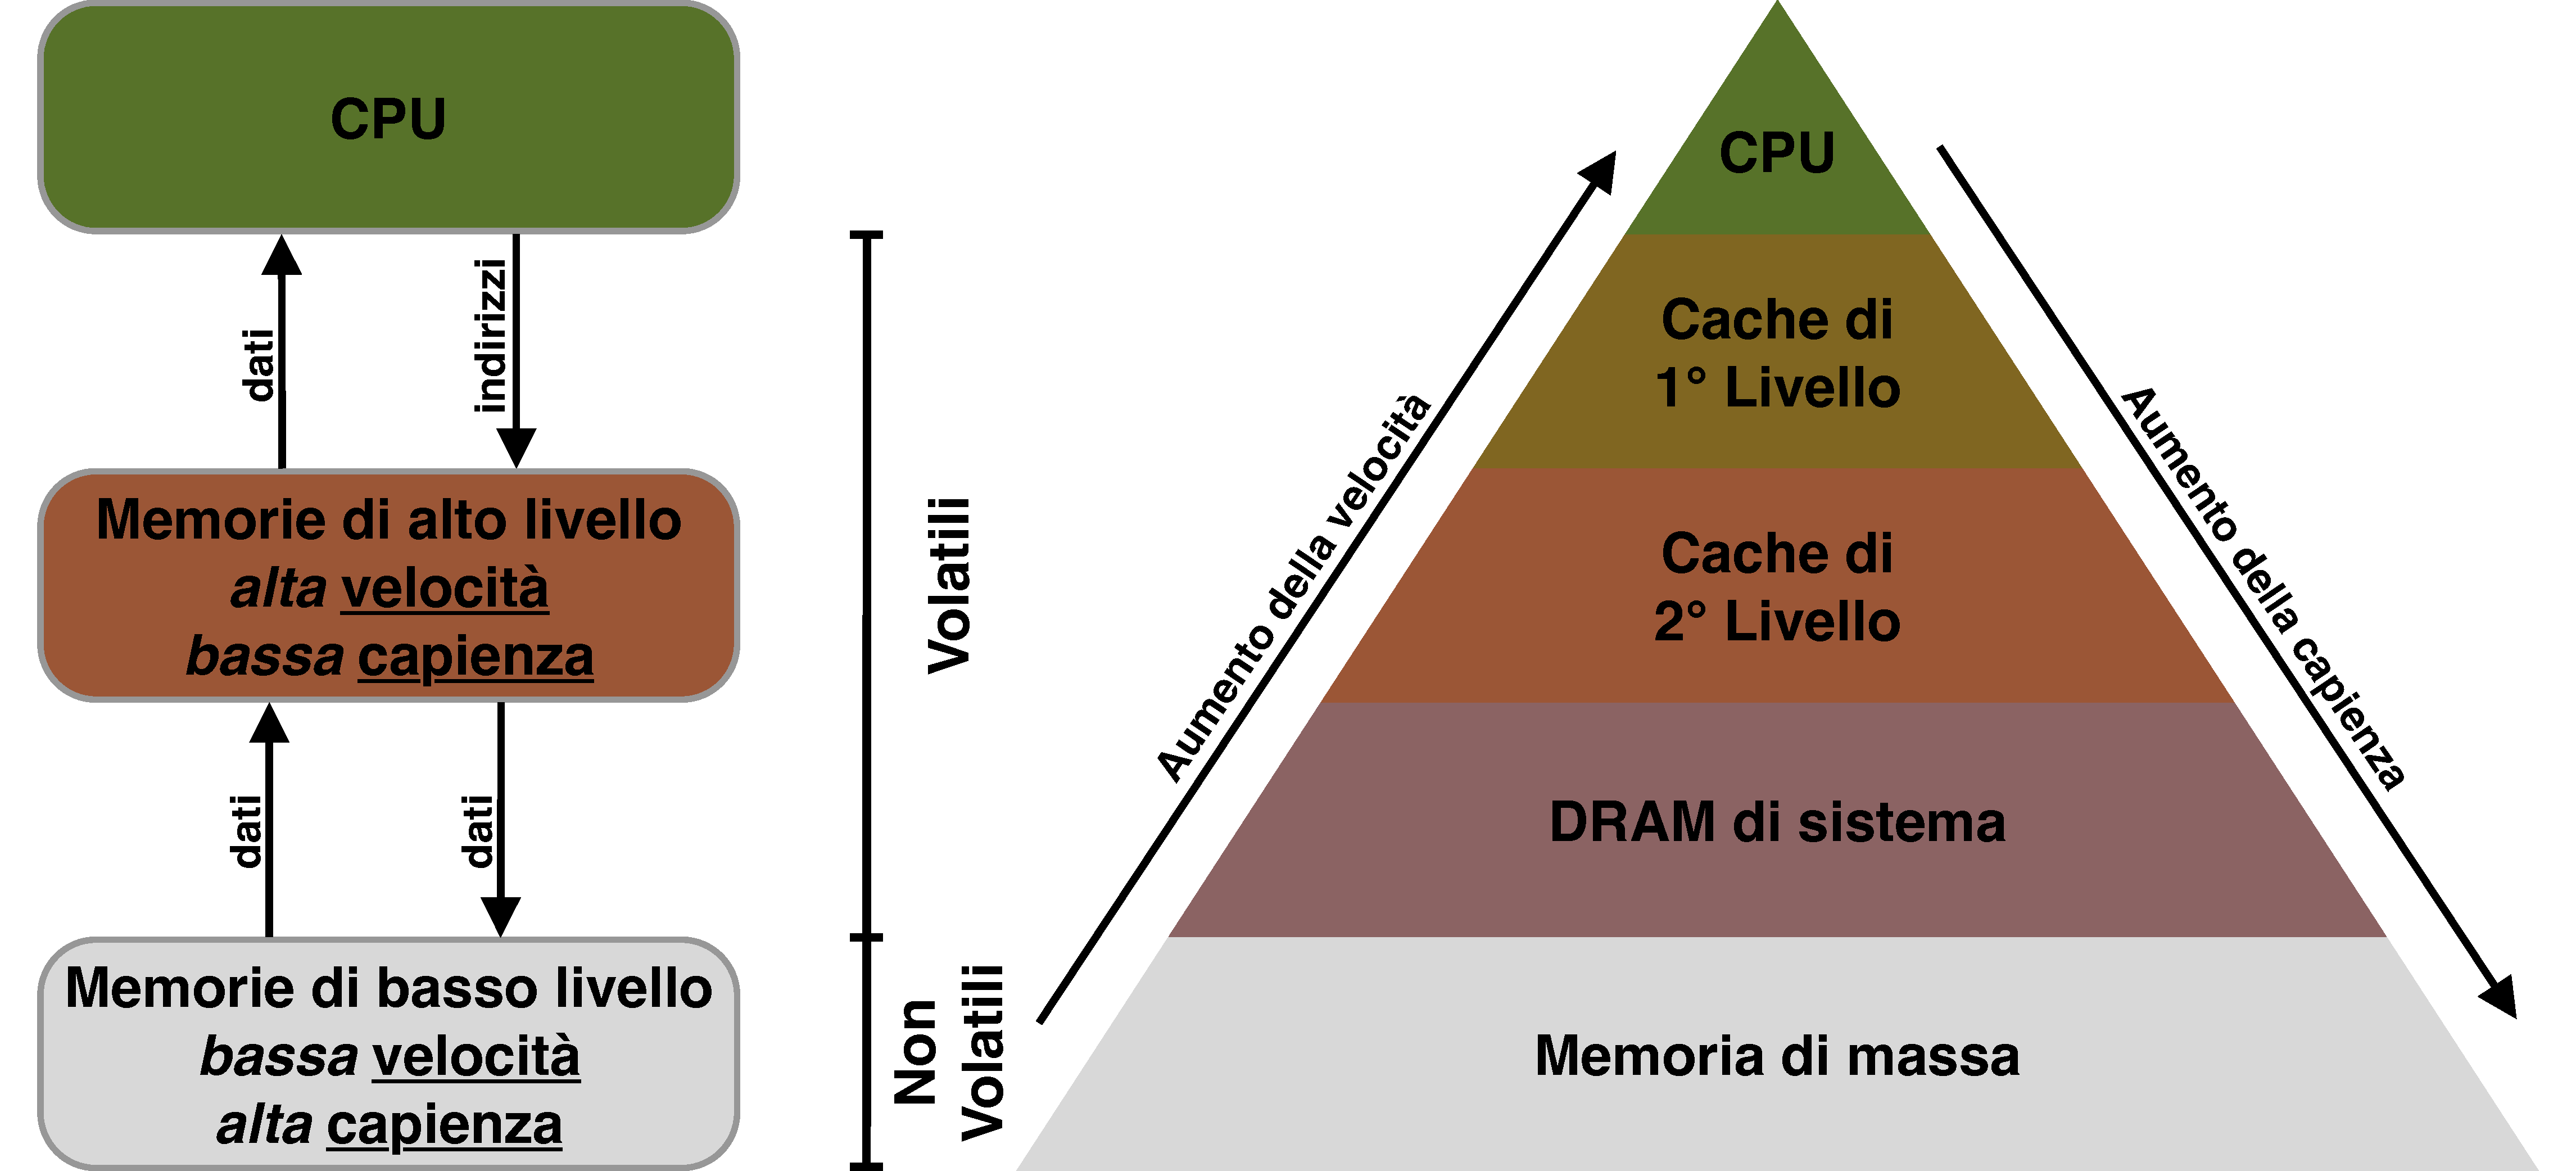
\includegraphics[width=0.7\linewidth]{images/5_memory/memory_hierarchy.pdf}
%		\caption{La CPU: CU, ALU e registri}
		\label{fig:memory_hierarchy}
	\end{figure} 

\end{frame}


\begin{frame}
	\frametitle{L'organizzazione in livelli gerarchici}

	\begin{figure}[!htbp] 
		\centering
		%\advance\leftskip-0.25cm
		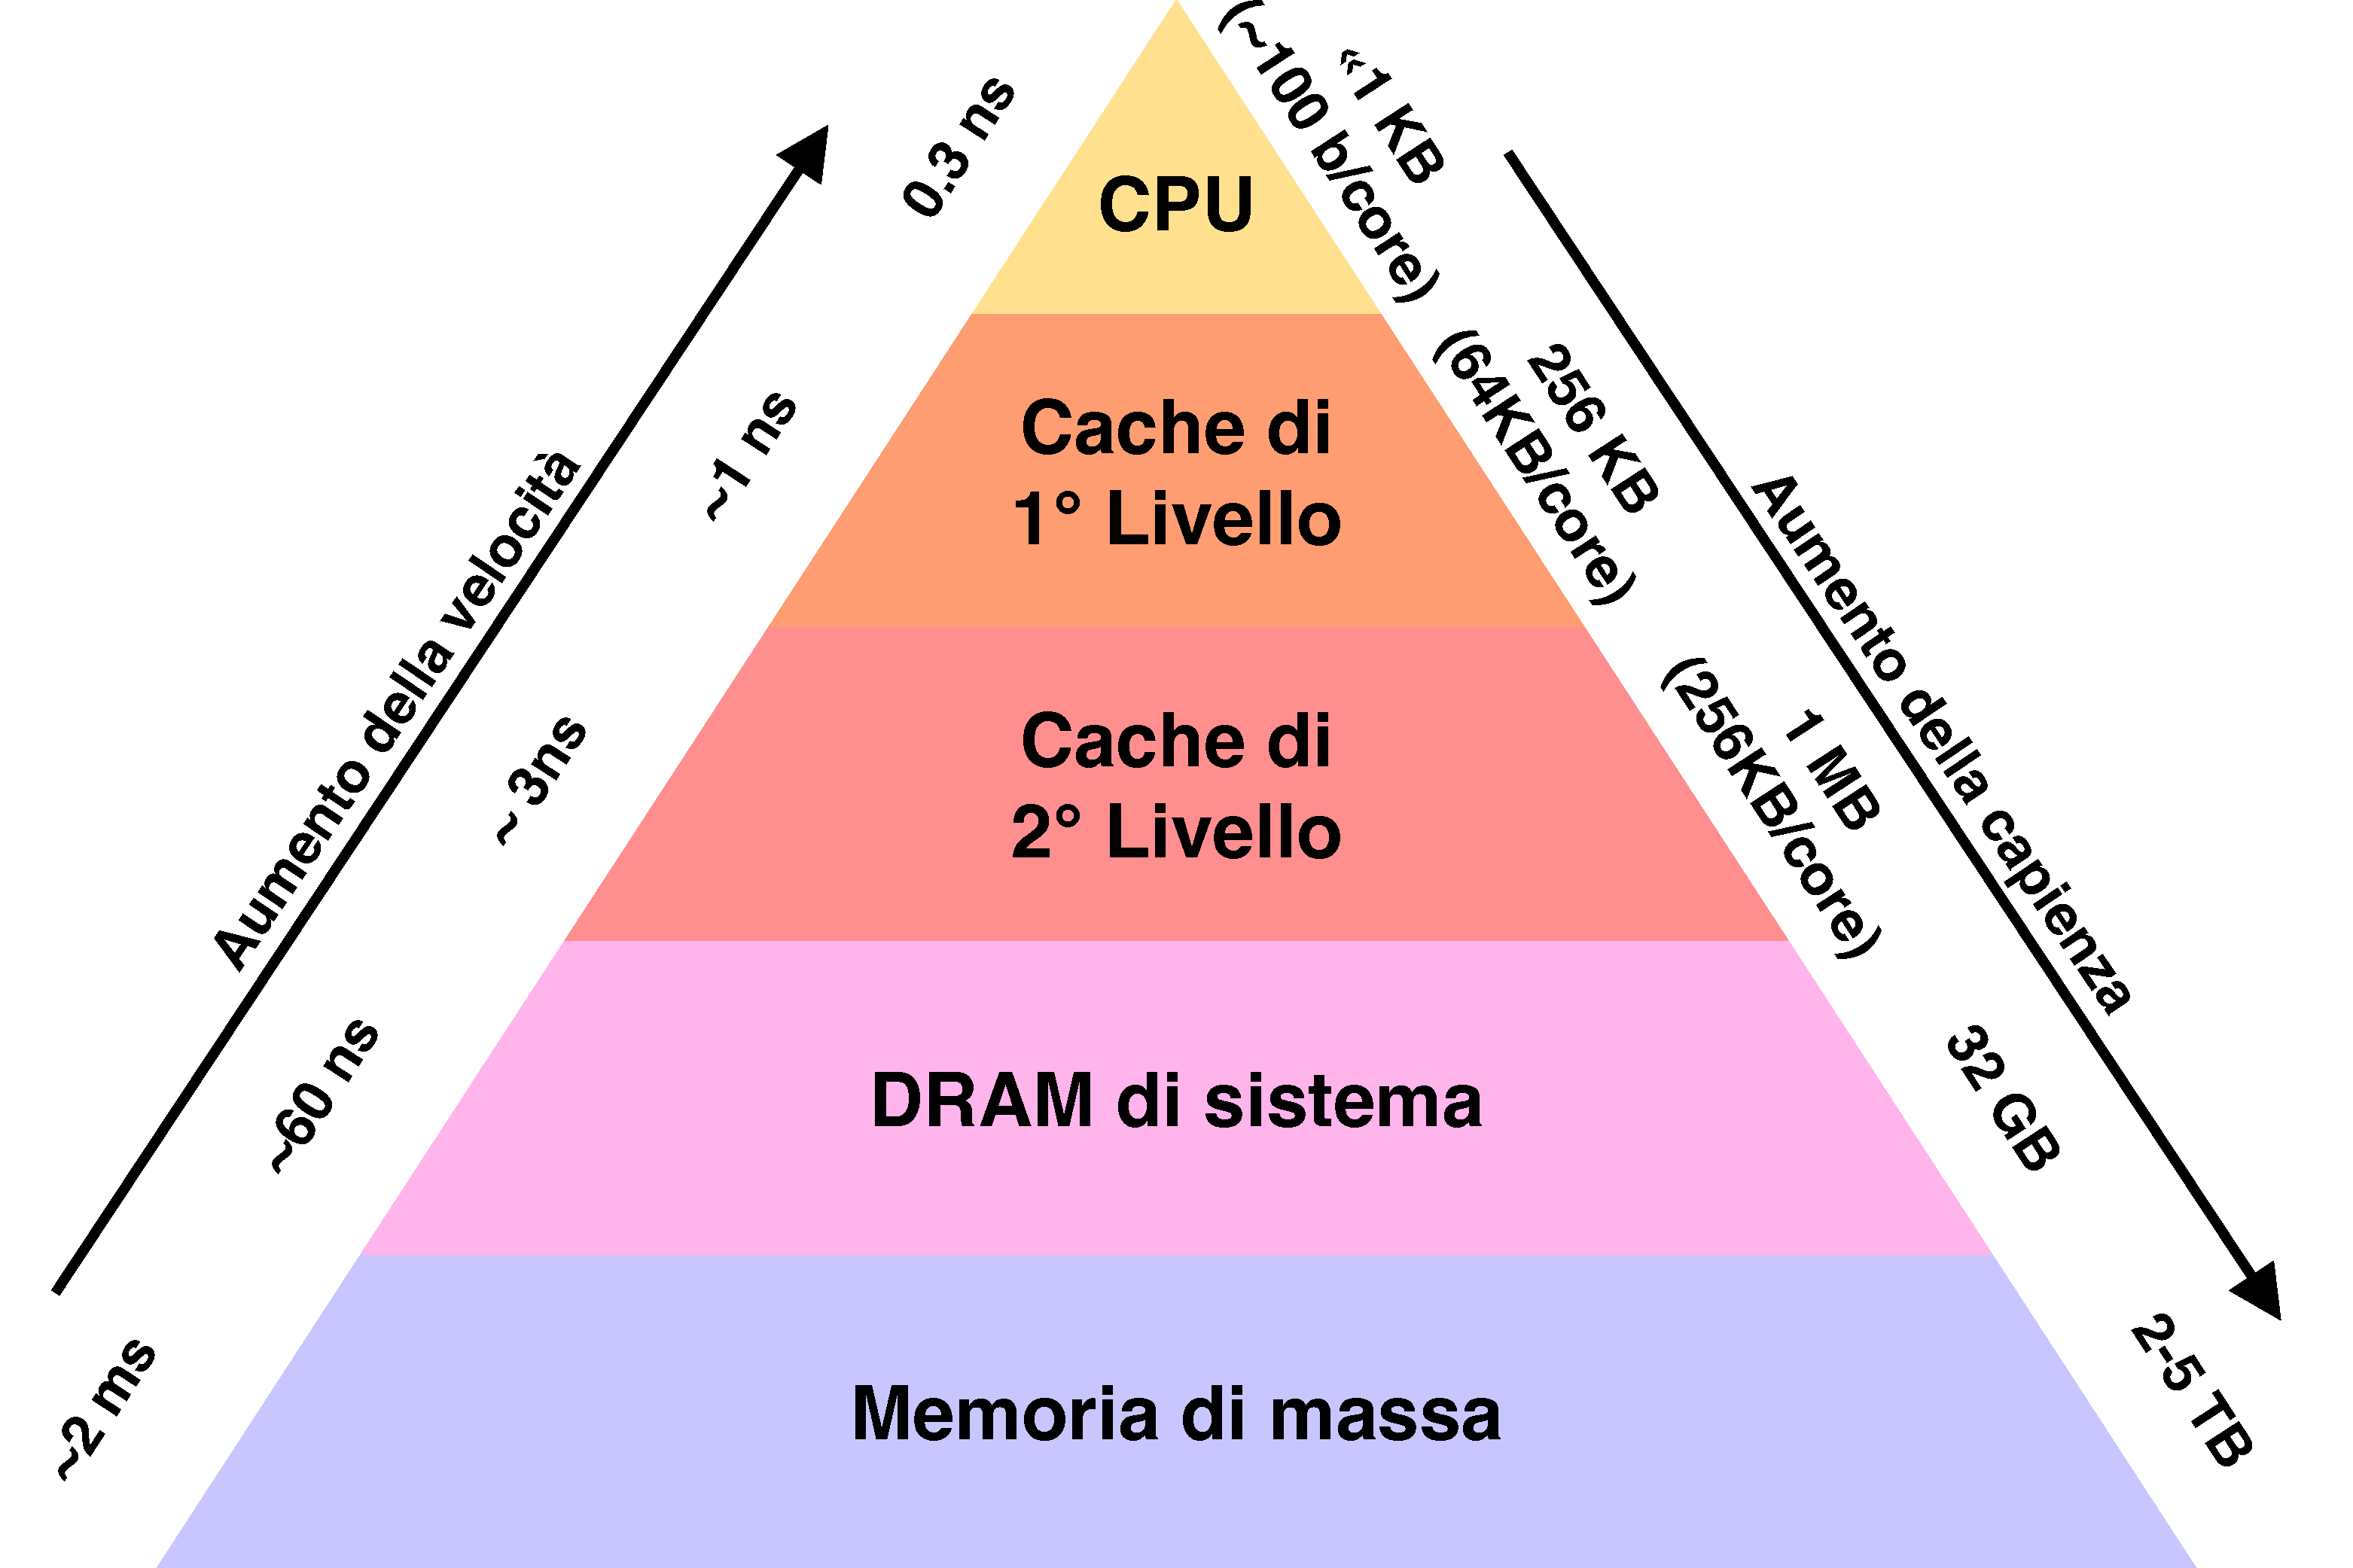
\includegraphics[width=0.9\linewidth]{images/5_memory/memory_hierarchy_info.pdf}
%		\caption{}
		\label{fig:memory_hierarchy}
	\end{figure} 

\end{frame}

\begin{frame}
	\frametitle{L'organizzazione in livelli gerarchici}
	 
	\begin{figure}[!htbp] 
		\centering
		%\advance\leftskip-0.25cm
		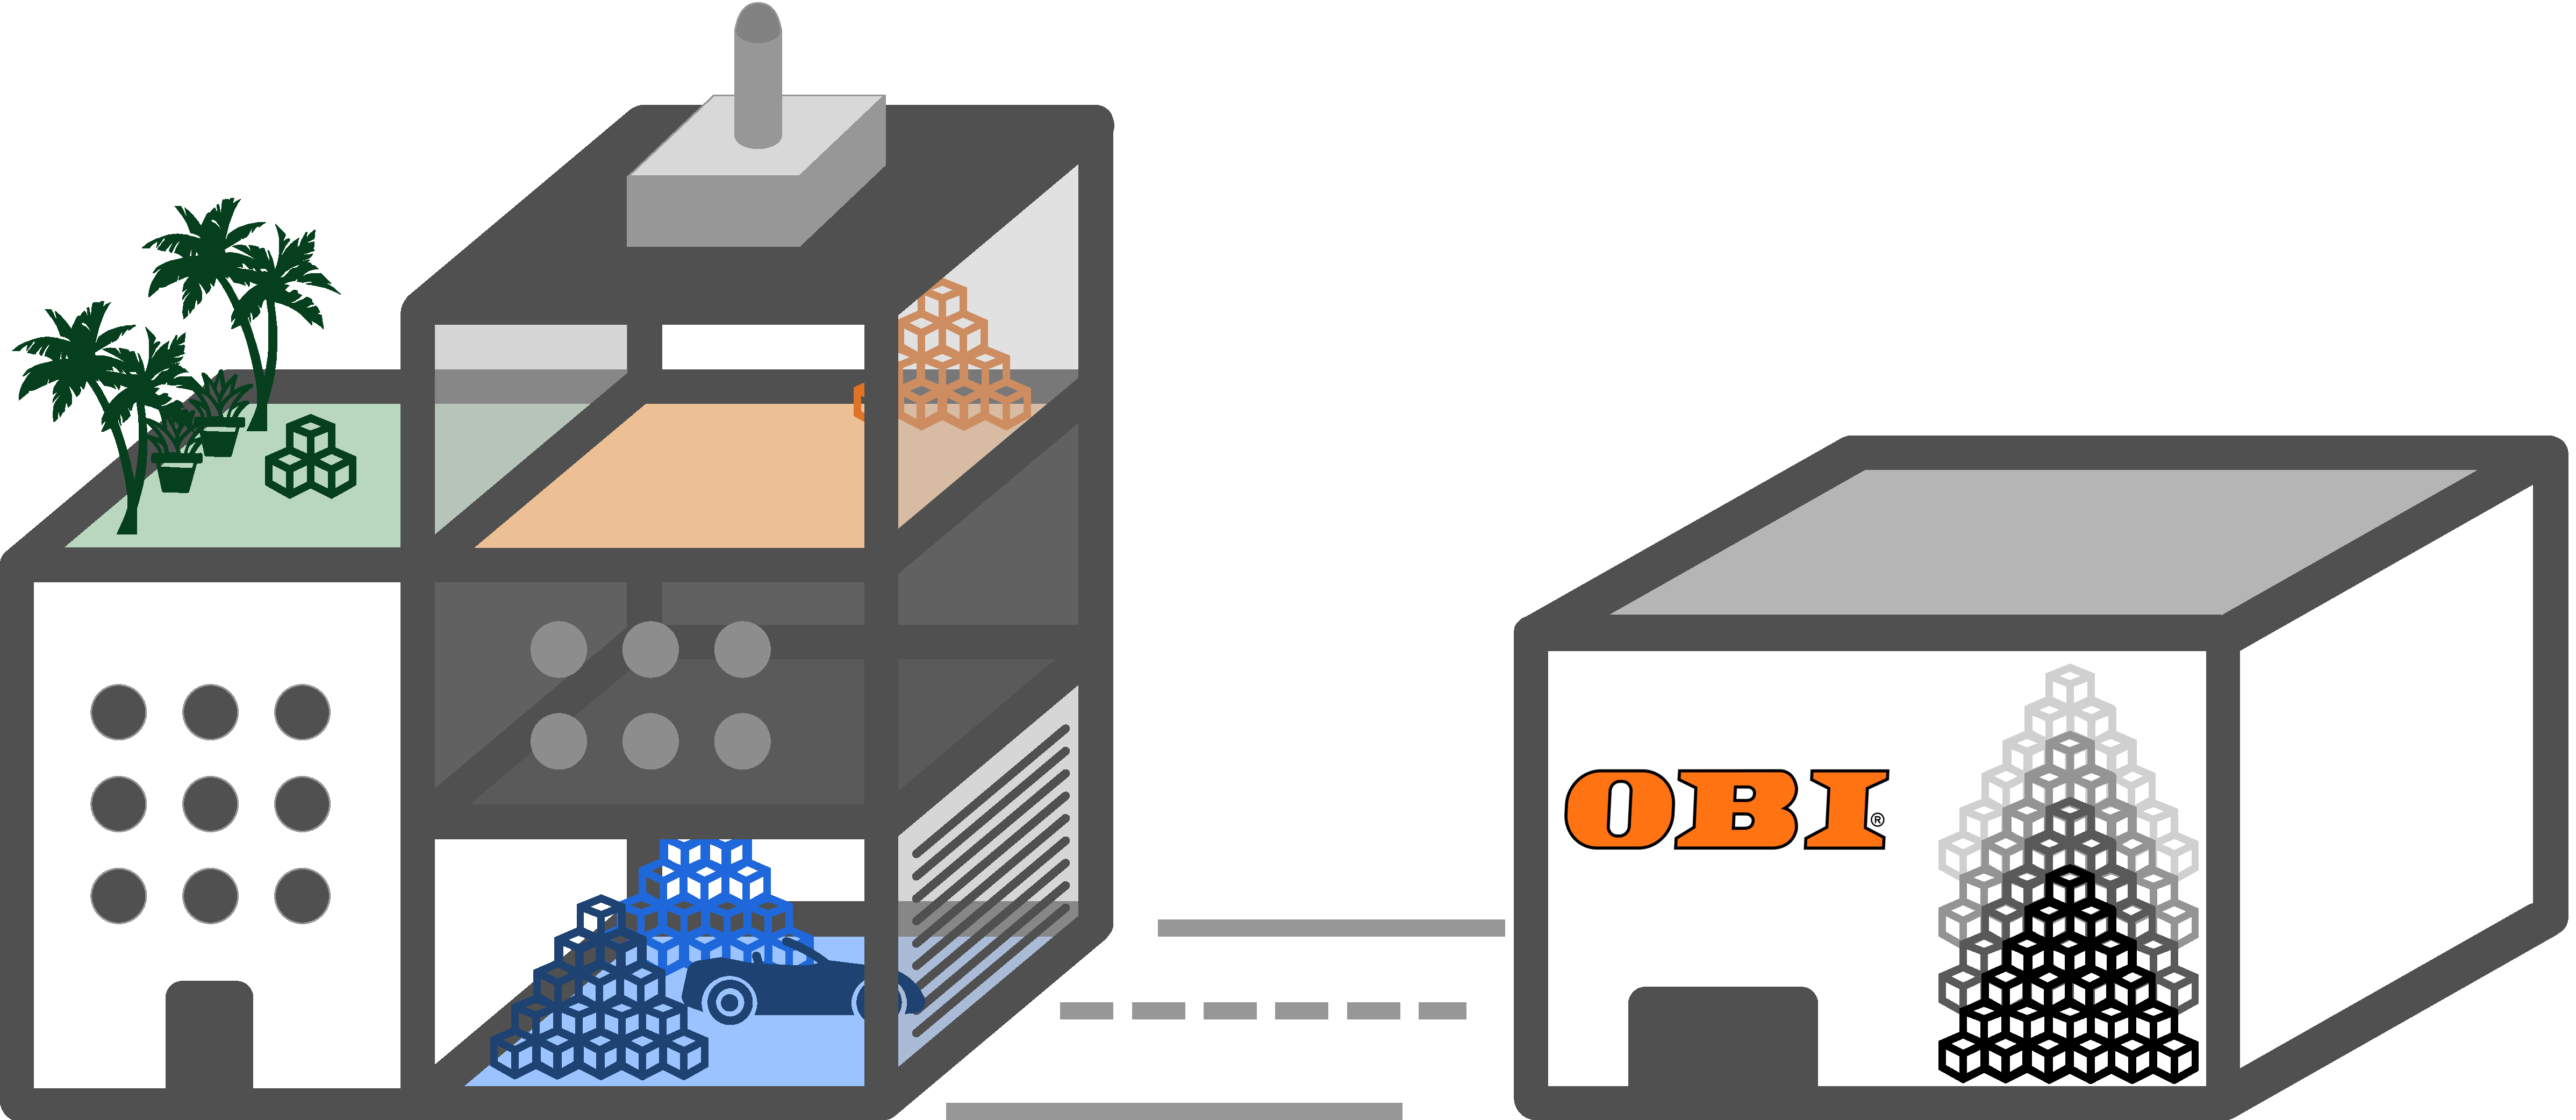
\includegraphics[width=1.0\linewidth]{images/5_memory/gardening.pdf}
		%\caption{}
	\end{figure}
	
\end{frame}

\begin{frame}
	\frametitle{L'organizzazione in livelli gerarchici}
	 
	 Immagina di vivere al terzo piano di un palazzo.\\
	 Vuoi fare giardinaggio sul tuo terrazzo, per lavorare hai bisogno di uno specifico attrezzo, ad esempio un rastrello. \pause
	 \begin{enumerate}
	 	\item se hai già un rastrello in uno dei cassetti per gli attrezzi del terrazzo (hit) procedi con i tuoi lavori, altrimenti (miss) \pause
	 	\item ti sposti in casa e cerchi il rastrello nei cassetti degli attrezzi del ripostiglio, se lo trovi (hit) torni sul terrazzo, altrimenti (miss) \pause
	 	\item ti sposti in garage e cerchi il rastrello nei cassetti degli attrezzi del garage, se lo trovi torni sul terrazzo, altrimenti (miss) \pause
	 	\item prendi la macchina e ti sposti all'OBI, cerchi il rastrello nei cassetti dell'OBI, se lo trovi torni sul terrazzo \pause
	 \end{enumerate}
	 Ogni volta che hai un hit copi questo e una piccola porzione adiacente ad essa nel livello superiore e così via fino a che non raggiungi il terrazzo. \pause
	 Ogni volta che hai un miss invece ti sposti a cercare nel livello inferiore.
	
\end{frame}


\begin{frame}
	\frametitle{L'organizzazione in livelli gerarchici}
	
	\begin{figure}[!htbp] 
		\centering
		%\advance\leftskip-0.25cm
		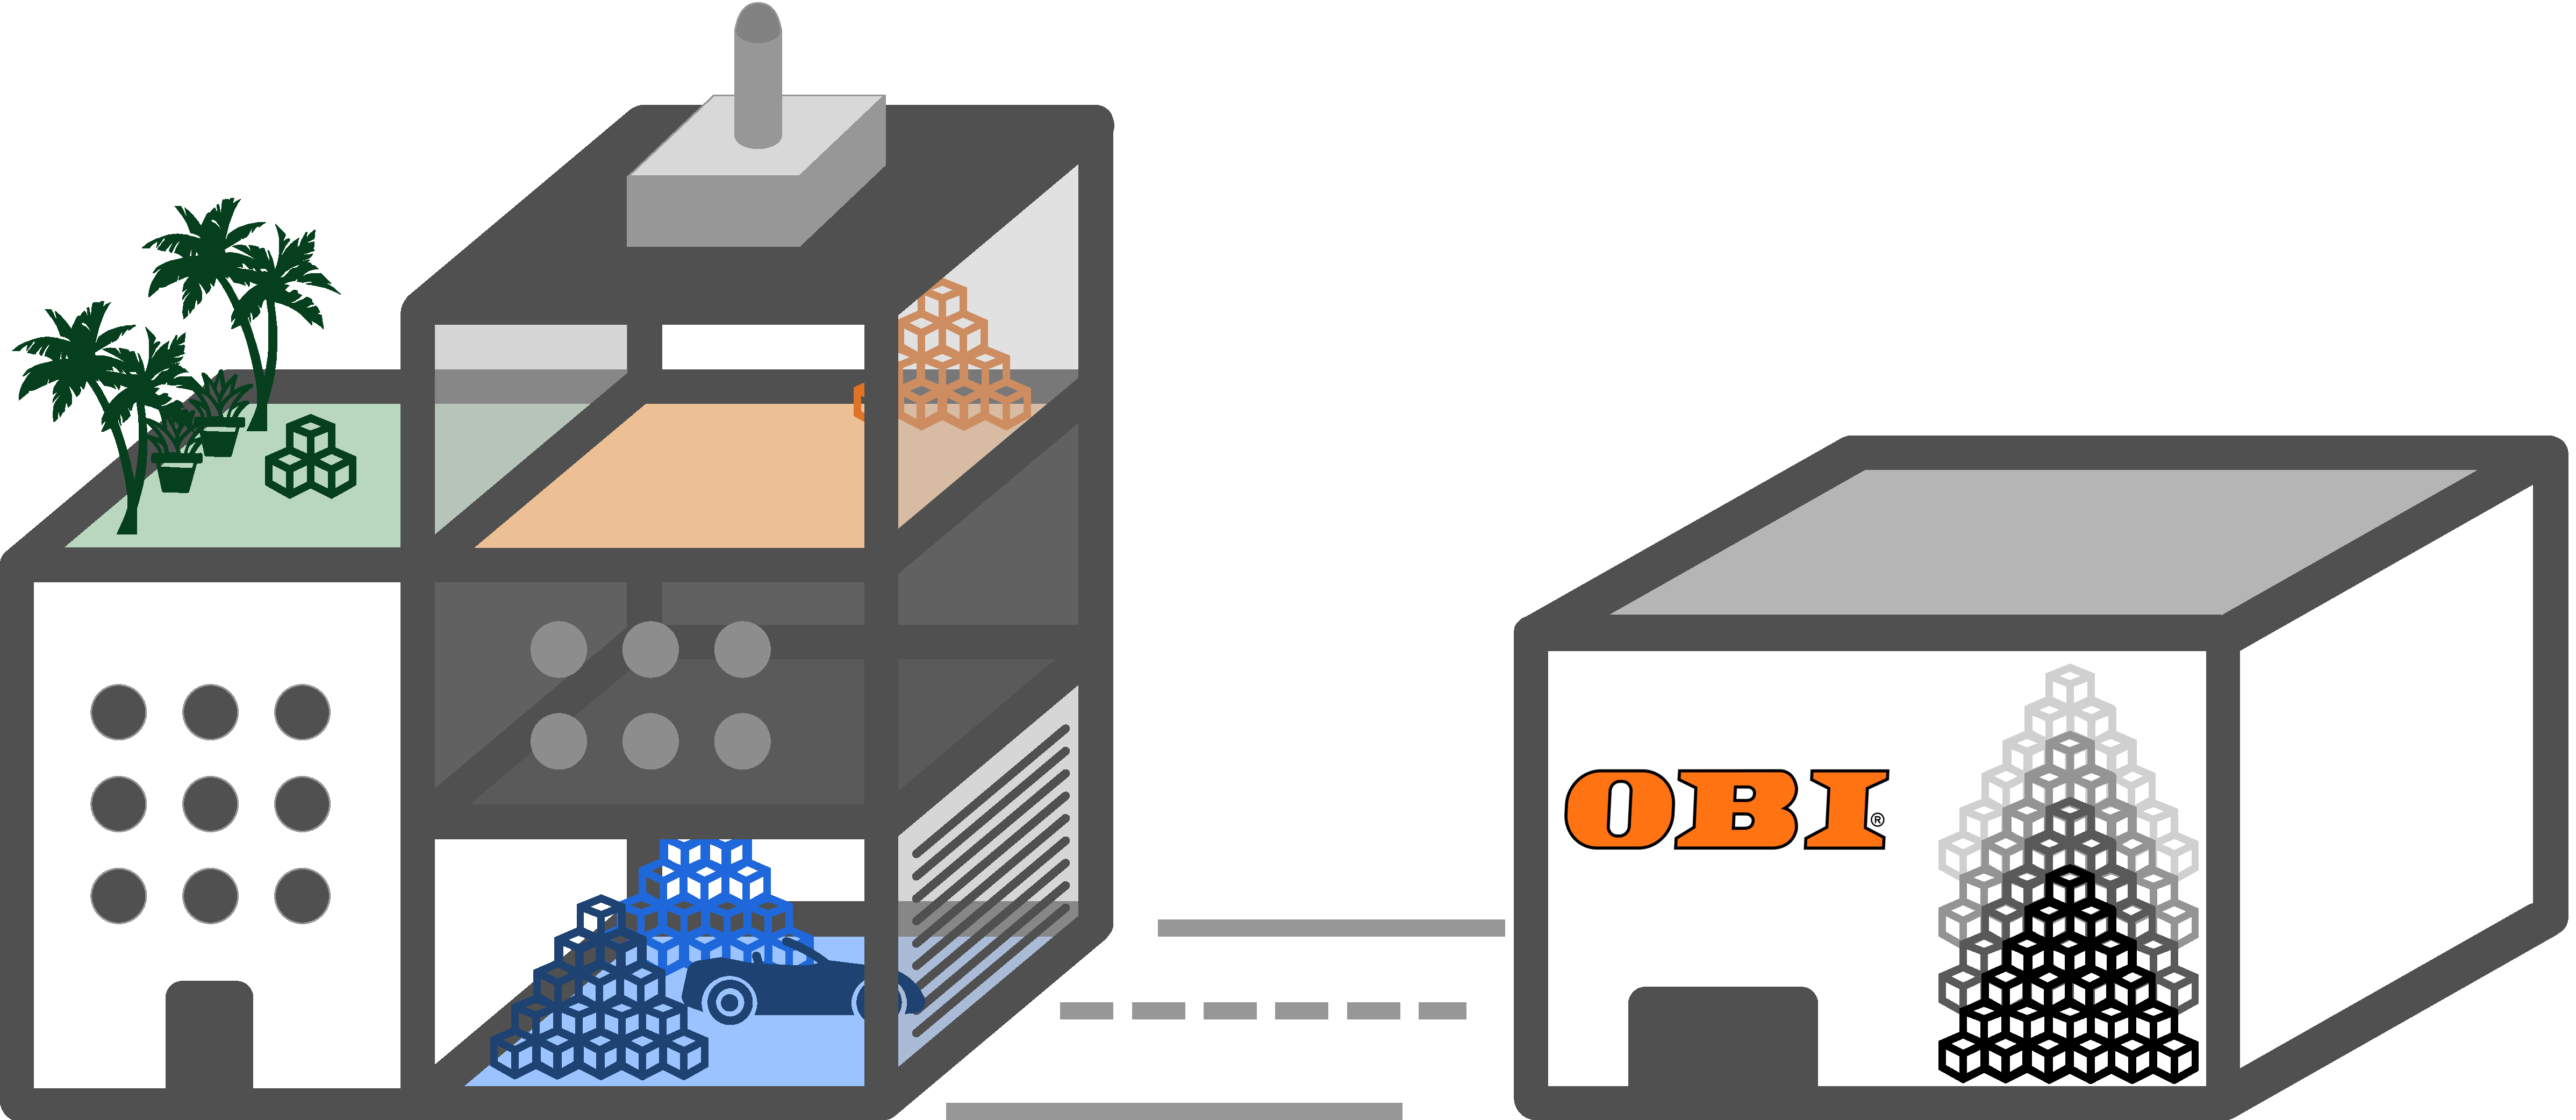
\includegraphics[width=0.6\linewidth]{images/5_memory/gardening.pdf}
		%\caption{}
	\end{figure}
	 \pause
	 Nell'esempio presentato: \pause
	 \begin{enumerate}
	 	\item il terrazzo e la abitazione: \pause \textbf{la CPU} \pause
	 	\item i cassetti degli attrezzi sul terrazzo: \pause \textbf{i registri} \pause
	 	\item i cassetti degli attrezzi nel ripostiglio: \pause la \textbf{memoria cache L1} \pause
	 	\item i cassetti degli attrezzi nel garage: \pause la \textbf{memoria cache L2} \pause
	 	\item i cassetti degli attrezzi da OBI: \pause la \textbf{RAM}
	 \end{enumerate}
	
\end{frame}


\subsubsection[Il tempo medio di accesso alla cache]{Il tempo medio di accesso alla cache}
\begin{frame}
	\frametitle{Il tempo medio di accesso alla cache}
	
	\begin{block}{Prestazioni di una memoria cache}
		Quando durante l’esecuzione di un processo, il processore genera un indirizzo, questo viene cercato in cache e si possono verificare 2 situazioni: \pause
		\begin{enumerate}
			\item l’indirizzo c'è (hit) \pause
			\item l’indirizzo non è presente (miss) \pause
		\end{enumerate}
		Per valutare la prestazione di una memoria cache si considerano: \pause
		\begin{itemize}
			\item \textbf{Hit rate ($h$)}: rapporto tra il numero di hit nel livello superiore e il numero totale dei riferimenti (prob. di avere un hit) \pause
			\item \textbf{Miss rate ($m$)}: rapporto tra il numero di miss nel livello superiore e il numero totale dei riferimenti (ricordiamo che $m=1-h$) \pause
			\item \textbf{Tempo di accesso alla cache ($t_c$)} \pause
			\item \textbf{Tempo di penalizzazione ($t_p$)}: tempo per accedere alla memoria centrale e per portare la linea in cache
		\end{itemize}
	\end{block}
	
\end{frame}

\begin{frame}
	\frametitle{Il tempo medio di accesso alla cache}
	
	\begin{block}{Il tempo medio di accesso alla cache $t$}
	Possiamo calcolare il \textbf{tempo medio di accesso alla cache} $t$ come segue:\vspace{0.25em} \pause
		\begin{Large}
		$$t = {\color{CpuGreen}h} \cdot {\color{CpuBlue}t_c} + {\color{CpuRed}m} \cdot {\color{CpuPink}t_p}$$
		\end{Large}
		~\vspace{0.5em} \pause
		Ovvero si calcola come: \pause
		\begin{enumerate}
			\item l'{\color{CpuGreen}\textbf{hit rate}} (prob. di hit) per il {\color{CpuBlue}\textbf{tempo di accesso alla memoria cache}} \pause
			\item più il \pause
			\item il {\color{CpuRed}\textbf{miss rate}} (prob. di miss = prob. di non hit) moltiplicato per il {\color{CpuPink}\textbf{tempo necessario ad ottenere il dato dalle memorie "inferiori"}} \pause
		\end{enumerate}
		
		Si noti che è una sorta di media pesata dove i pesi sono dati da $h$ e $m$, ovvero hit rate e miss rate che sono due probabilità tali che ${\color{CpuGreen}h} + {\color{CpuRed}m} = 1$.
	\end{block}
	
\end{frame}


\begin{frame}
	\frametitle{Esercizi sul tempo medio di accesso alla cache}
	
	\begin{block}{Esercizio 1: calcola il $t_p$ (miss penalty)}
		La memoria cache di un server ha:
			\begin{itemize}
				\item \textbf{Hit rate} di 82\% \hspace{10em} $\rightarrow$ \hspace{2em} ${\color{CpuGreen}h} = 0.8$
				\item \textbf{Tempo medio di accesso} di 80 ns \hspace{2em} $\rightarrow$ \hspace{2em} $t = 80ns$
				\item \textbf{Hit time} di 15ns \hspace{9.7em} $\rightarrow$ \hspace{2em} ${\color{CpuBlue}t_c} = 15ns$
			\end{itemize}
		~\\ \pause
		Qual è il valore di Miss Penalty della cache (${\color{CpuPink}t_p}$)?
		\begin{itemize}
			\item A. Circa 500 ns
			\item B. Circa 376ns
			\item C. Maggiore di 3,76 ms
			\item D. Minore di 300 ns
		\end{itemize}
	\end{block}

\end{frame}


\begin{frame}
	\frametitle{Esercizi sul tempo medio di accesso alla cache}
	
	\begin{block}{Esercizio 1: calcola il $t_p$ (miss penalty)}
		Prendiamo la formula della precedente slide:
		$$t = {\color{CpuGreen}h} \cdot {\color{CpuBlue}t_c} + {\color{CpuRed}m} \cdot {\color{CpuPink}t_p}$$
		\pause
		Ed invertiamola ricavando il ${\color{CpuPink}t_p}$ (miss penalty):
		$${\color{CpuPink}t_p} = \pause \frac{t - {\color{CpuGreen}h} \cdot {\color{CpuBlue}t_c}}{{\color{CpuRed}m}} \pause = \frac{t - {\color{CpuGreen}h} \cdot {\color{CpuBlue}t_c}}{1 - {\color{CpuGreen}h}}$$
		\pause
		Da cui, sostituendo i valori numerici:
		\pause
		$${\color{CpuPink}t_p} = \frac{80 - {\color{CpuGreen}0.82} \cdot {\color{CpuBlue}15}}{1 - {\color{CpuGreen}0.82}} = 376.11 ns$$
	\end{block}

\end{frame}



\begin{frame}
	\frametitle{Esercizi sul tempo medio di accesso alla cache}
	
	\begin{block}{Esercizio 2: calcola il $t$ (tempo medio di accesso)}
		La memoria cache di un server ha:
			\begin{itemize}
				\item \textbf{Hit rate} di 82\% \hspace{9.5em} $\rightarrow$ \hspace{2em} ${\color{CpuGreen}h} = 0.8$
				\item \textbf{Hit time} di 2ns \hspace{9.7em} $\rightarrow$ \hspace{2em} ${\color{CpuBlue}t_c} = 2ns$
				\item \textbf{Miss penalty} di 500ns \hspace{6.8em} $\rightarrow$ \hspace{2em} ${\color{CpuPink}t_p} = 500ns$
			\end{itemize}
		\end{block}
		\pause
		$$t = {\color{CpuGreen}h} \cdot {\color{CpuBlue}t_c} + {\color{CpuRed}m} \cdot {\color{CpuPink}t_p}$$
		\pause
		Da cui, sostituendo i valori numerici:
		\pause
		$$\qquad \qquad t = {\color{CpuGreen}0.8} \cdot {\color{CpuBlue}2} + {\color{CpuRed}0.2} \cdot {\color{CpuPink}500} = 101.6ns \quad \pause (\ll 500ns)$$
	

\end{frame}


\subsubsection[I principi di località: spaziale e temporale]{I principi di località: spaziale e temporale}
\begin{frame}
%	\frametitle{I flip-flop}
	
	\begin{block}{I principi di località}
		I \textbf{principi di località}, sono concetti chiave nelle memorie cache per ottimizzare l'efficienza dell'accesso ai dati. Essi si basano sull'osservazione che i pattern di accesso alle memorie tendono ad avere delle caratteristiche prevedibili che possono essere sfruttate per migliorare le prestazioni complessive.
		\begin{itemize}
			\item \textbf{Località Spaziale}: dati adiacenti ai recenti accessi vengono probabilmente richiesti poiché le istruzioni spesso accedono a dati correlati e contigui nello spazio.
			\item \textbf{Località Temporale}: dati acceduti di recente hanno alta probabilità di essere richiesti nuovamente entro breve tempo (ad esempio in caso di cicli).
		\end{itemize}
		Queste due sono la ragione per cui quando si ha un cache-miss si carica nella cache non solo il dato mancante, ma anche molti altri dati ad esso adiacenti (il blocco).
	\end{block}
		
\end{frame}




\subsection[I tipi di memoria]{I tipi di memoria}
\begin{frame}
%	\frametitle{I tipi di memoria}
	\begin{figure}[!htbp] 
		\centering
		%\advance\leftskip-0.25cm
		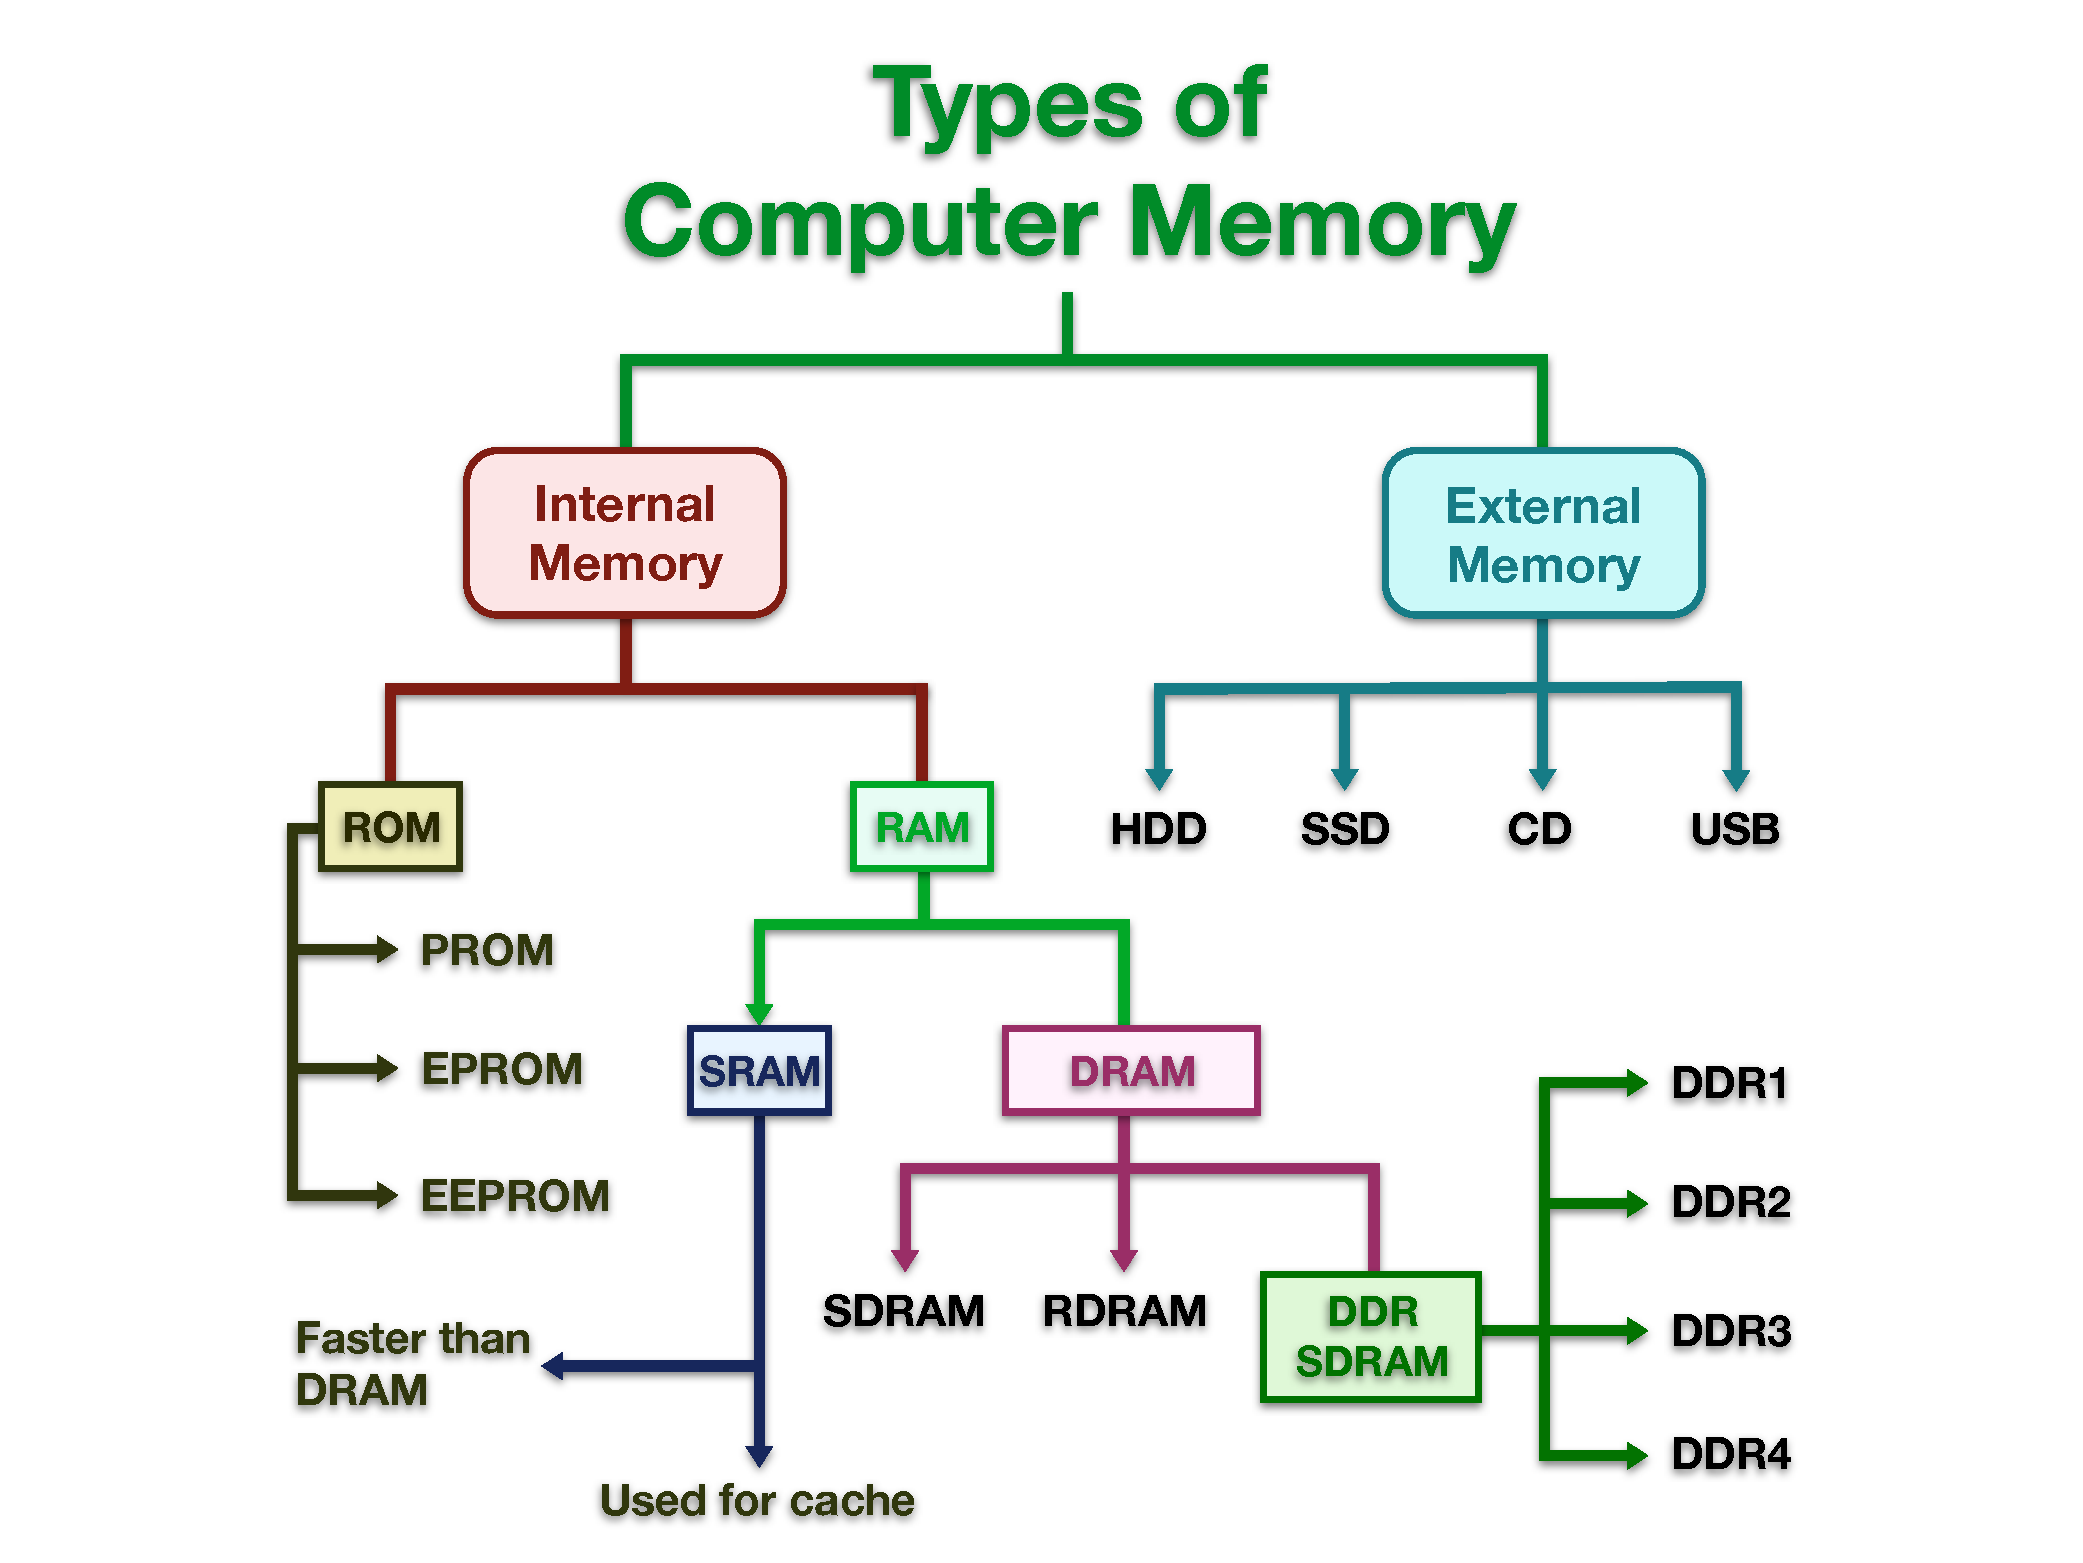
\includegraphics[width=0.95\linewidth]{images/5_memory/memory_types.pdf}
%		\caption{}
	\end{figure}
		
\end{frame}


\subsection[I flip-flop]{I flip-flop}
\begin{frame}
%	\frametitle{I flip-flop}
	
	\begin{block}{I flip-flop}
		Esistono diverse tecnologie per la realizzazione dei circuiti di memoria. Uno dei dispositivi elettronici più semplici per la memorizzazione dei bit è il \textbf{flip-flop}. Il flip-flop è una delle possibili implementazioni della \textbf{cella di memoria elementare} volatile. \\ Ricordiamo che il bit è la più piccola unità di informazione elettronica che possiamo memorizzare.
	\end{block}
	
	\begin{block}{I flip-flop SR (detti SR Latch)}
		Il \textbf{flip-flop SR}, noto anche come \textbf{SR Latch}, può essere considerato uno dei circuiti logici sequenziali più basilari possibili. Questo semplice flip-flop è fondamentalmente un dispositivo bistabile di memoria a un bit che ha due ingressi:
		\begin{itemize} 
			\item \textbf{S}: che prende il nome di \textbf{set}, che imposta l'uscita a 1
			\item \textbf{R}: che prende il nome di \textbf{reset}, che imposta l'uscita a 0
		\end{itemize}
	\end{block}
	
\end{frame}


\subsubsection[Flip-flop SR - NOR Gate]{Flip-flop SR - NOR Gate}
\begin{frame}
	\frametitle{Flip-flop SR - NOR Gate}
	 
	\begin{figure}[!htbp] 
		\centering
		%\advance\leftskip-0.25cm
		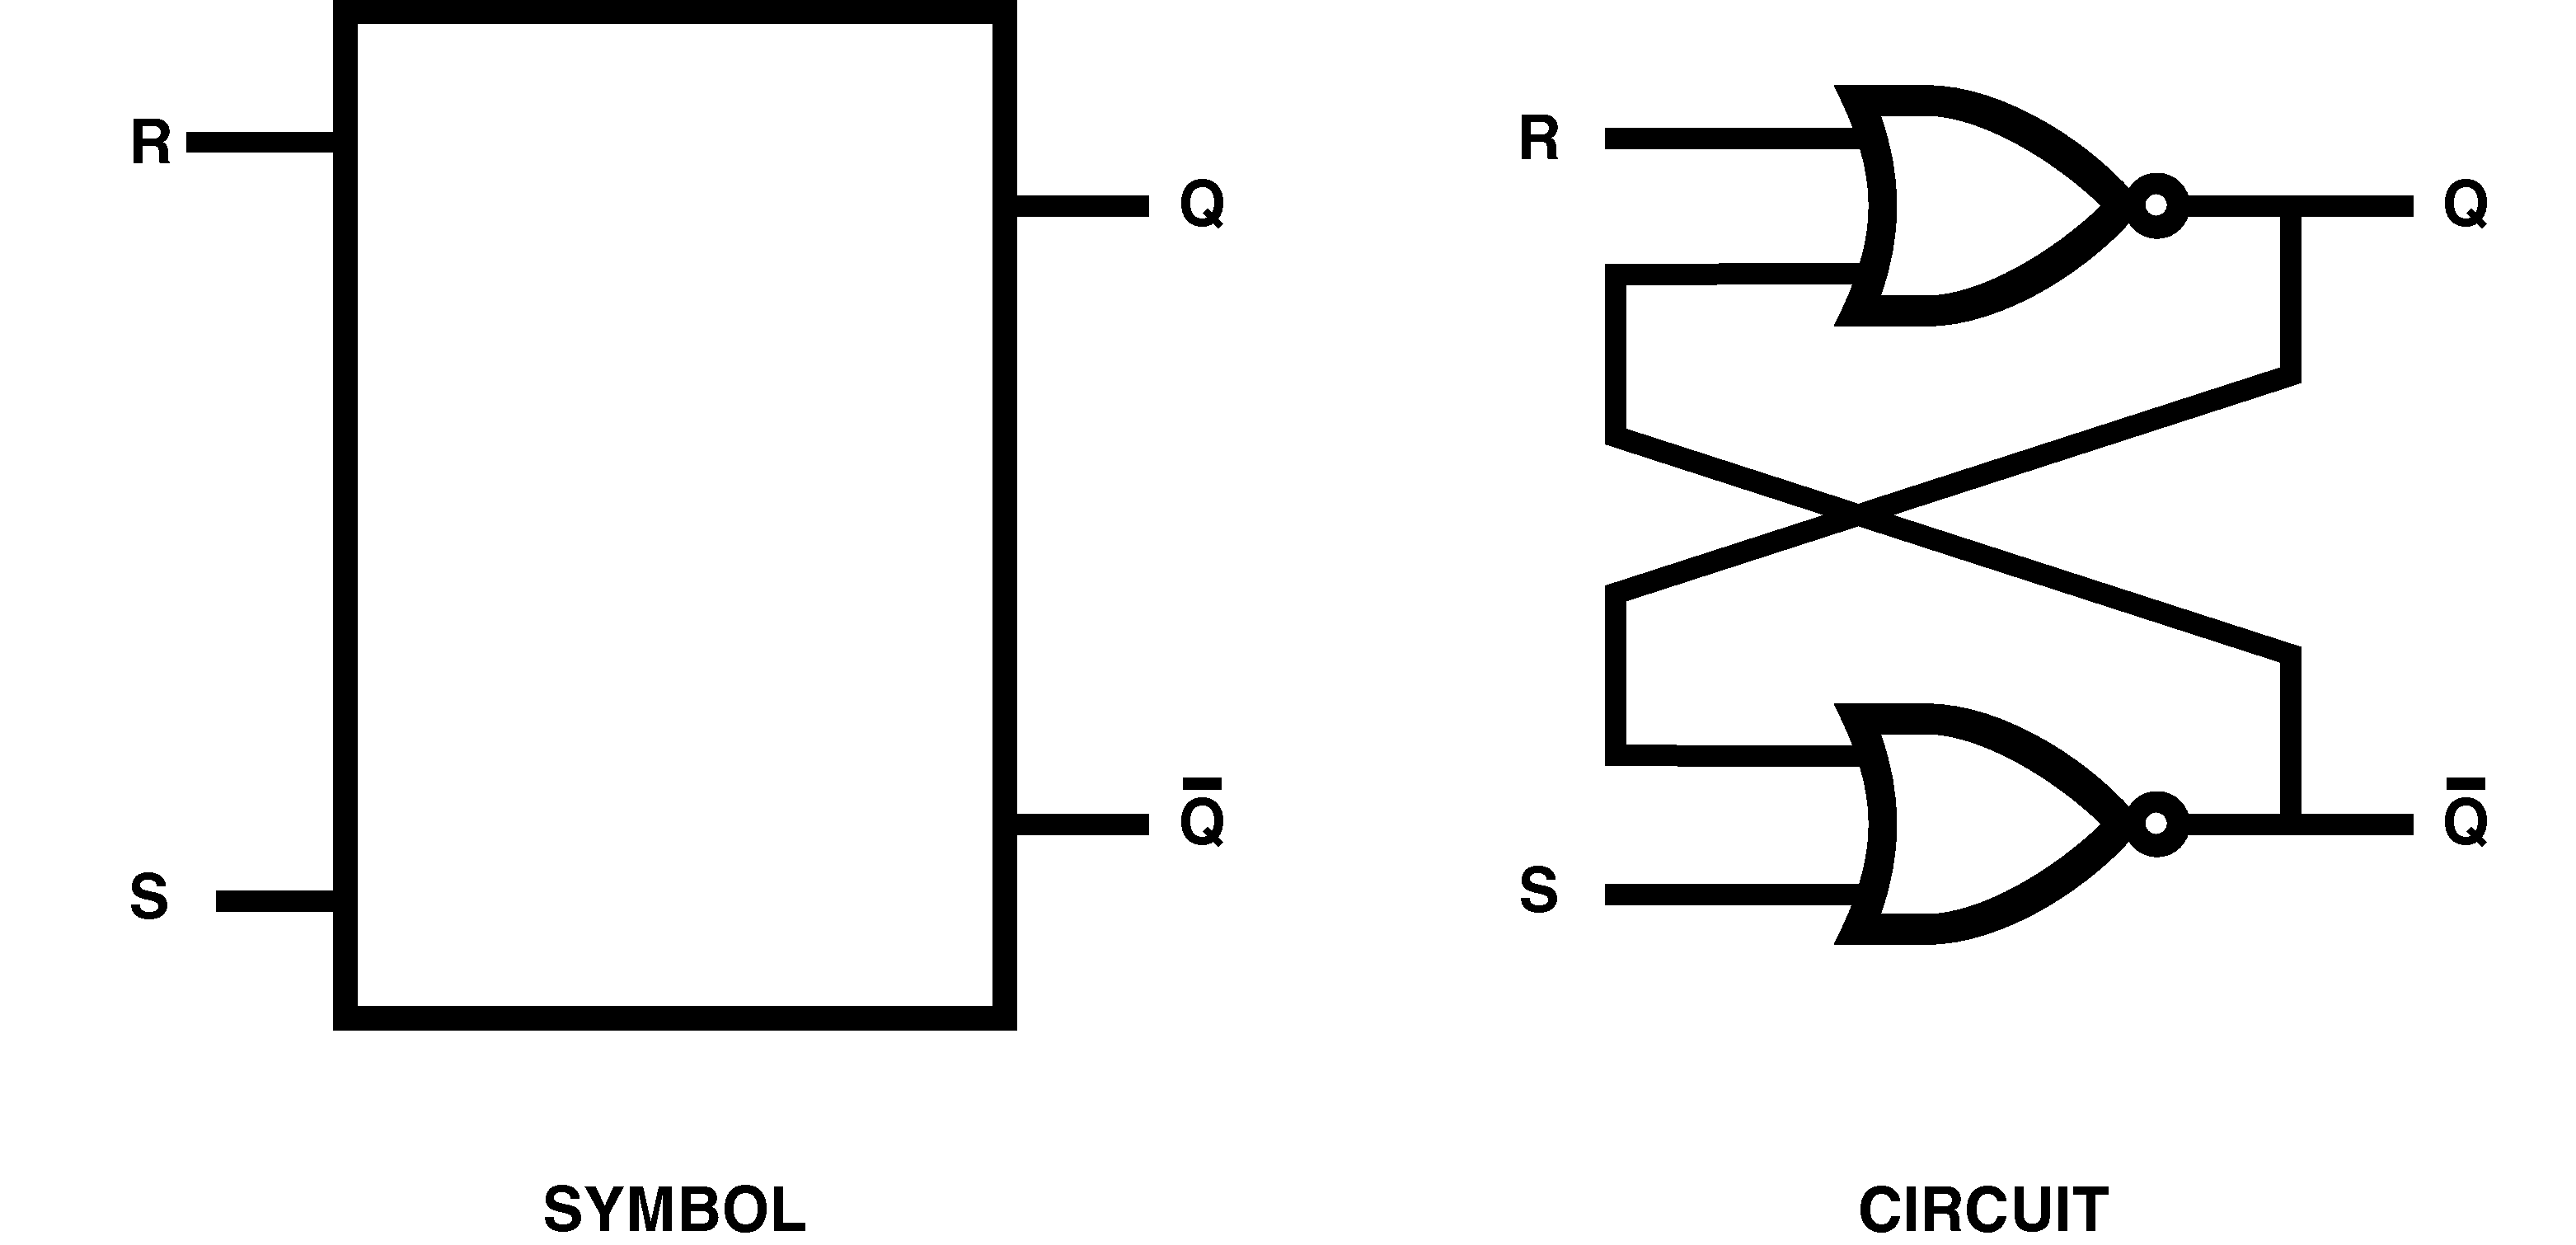
\includegraphics[width=0.95\linewidth]{images/5_memory/flip_flop_sr_nor.pdf}
		\caption{Il flip-flop SR: vedi il \underline{\href{https://www.youtube.com/watch?v=br2pbjAnP2k}{video su youtube}}}
	\end{figure}
	
\end{frame}

\begin{frame}
	\frametitle{Flip-flop SR - NOR Gate}
	 
	\begin{figure}[!htbp] 
		\centering
		%\advance\leftskip-0.25cm
		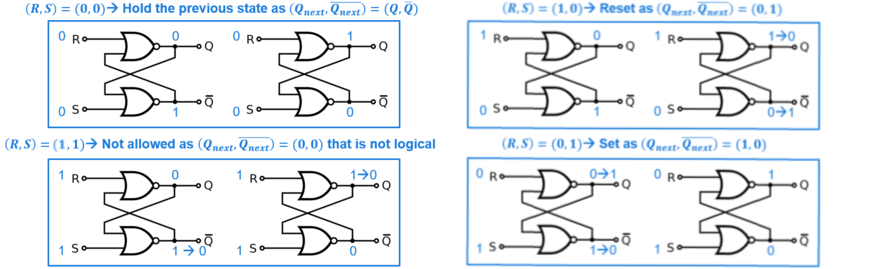
\includegraphics[width=1.0\linewidth]{images/5_memory/flip_flop_sr_nor.png}
		\caption{Il flip-flop SR con NOR, esempi}
	\end{figure}
	
\end{frame}

\begin{frame}

	\frametitle{Flip-flop SR - NOR Gate}

%	\begin{block}{K-means: algoritmo}
		\centering
		\animategraphics[controls={play, step, stop}, height=7cm]{3.0}{images/5_memory/flip_flop_sr_nor/flip_flop_sr_nor-}{0}{15}
		\label{fig:flip_flop_sr_nor}
%	\end{block}

\end{frame}


\subsubsection[Flip-flop SR - NAND Gate]{Flip-flop SR - NAND Gate}
\begin{frame}
	\frametitle{Flip-flop SR - NAND Gate}
	 
	\begin{figure}[!htbp]  
		\centering
		%\advance\leftskip-0.25cm
		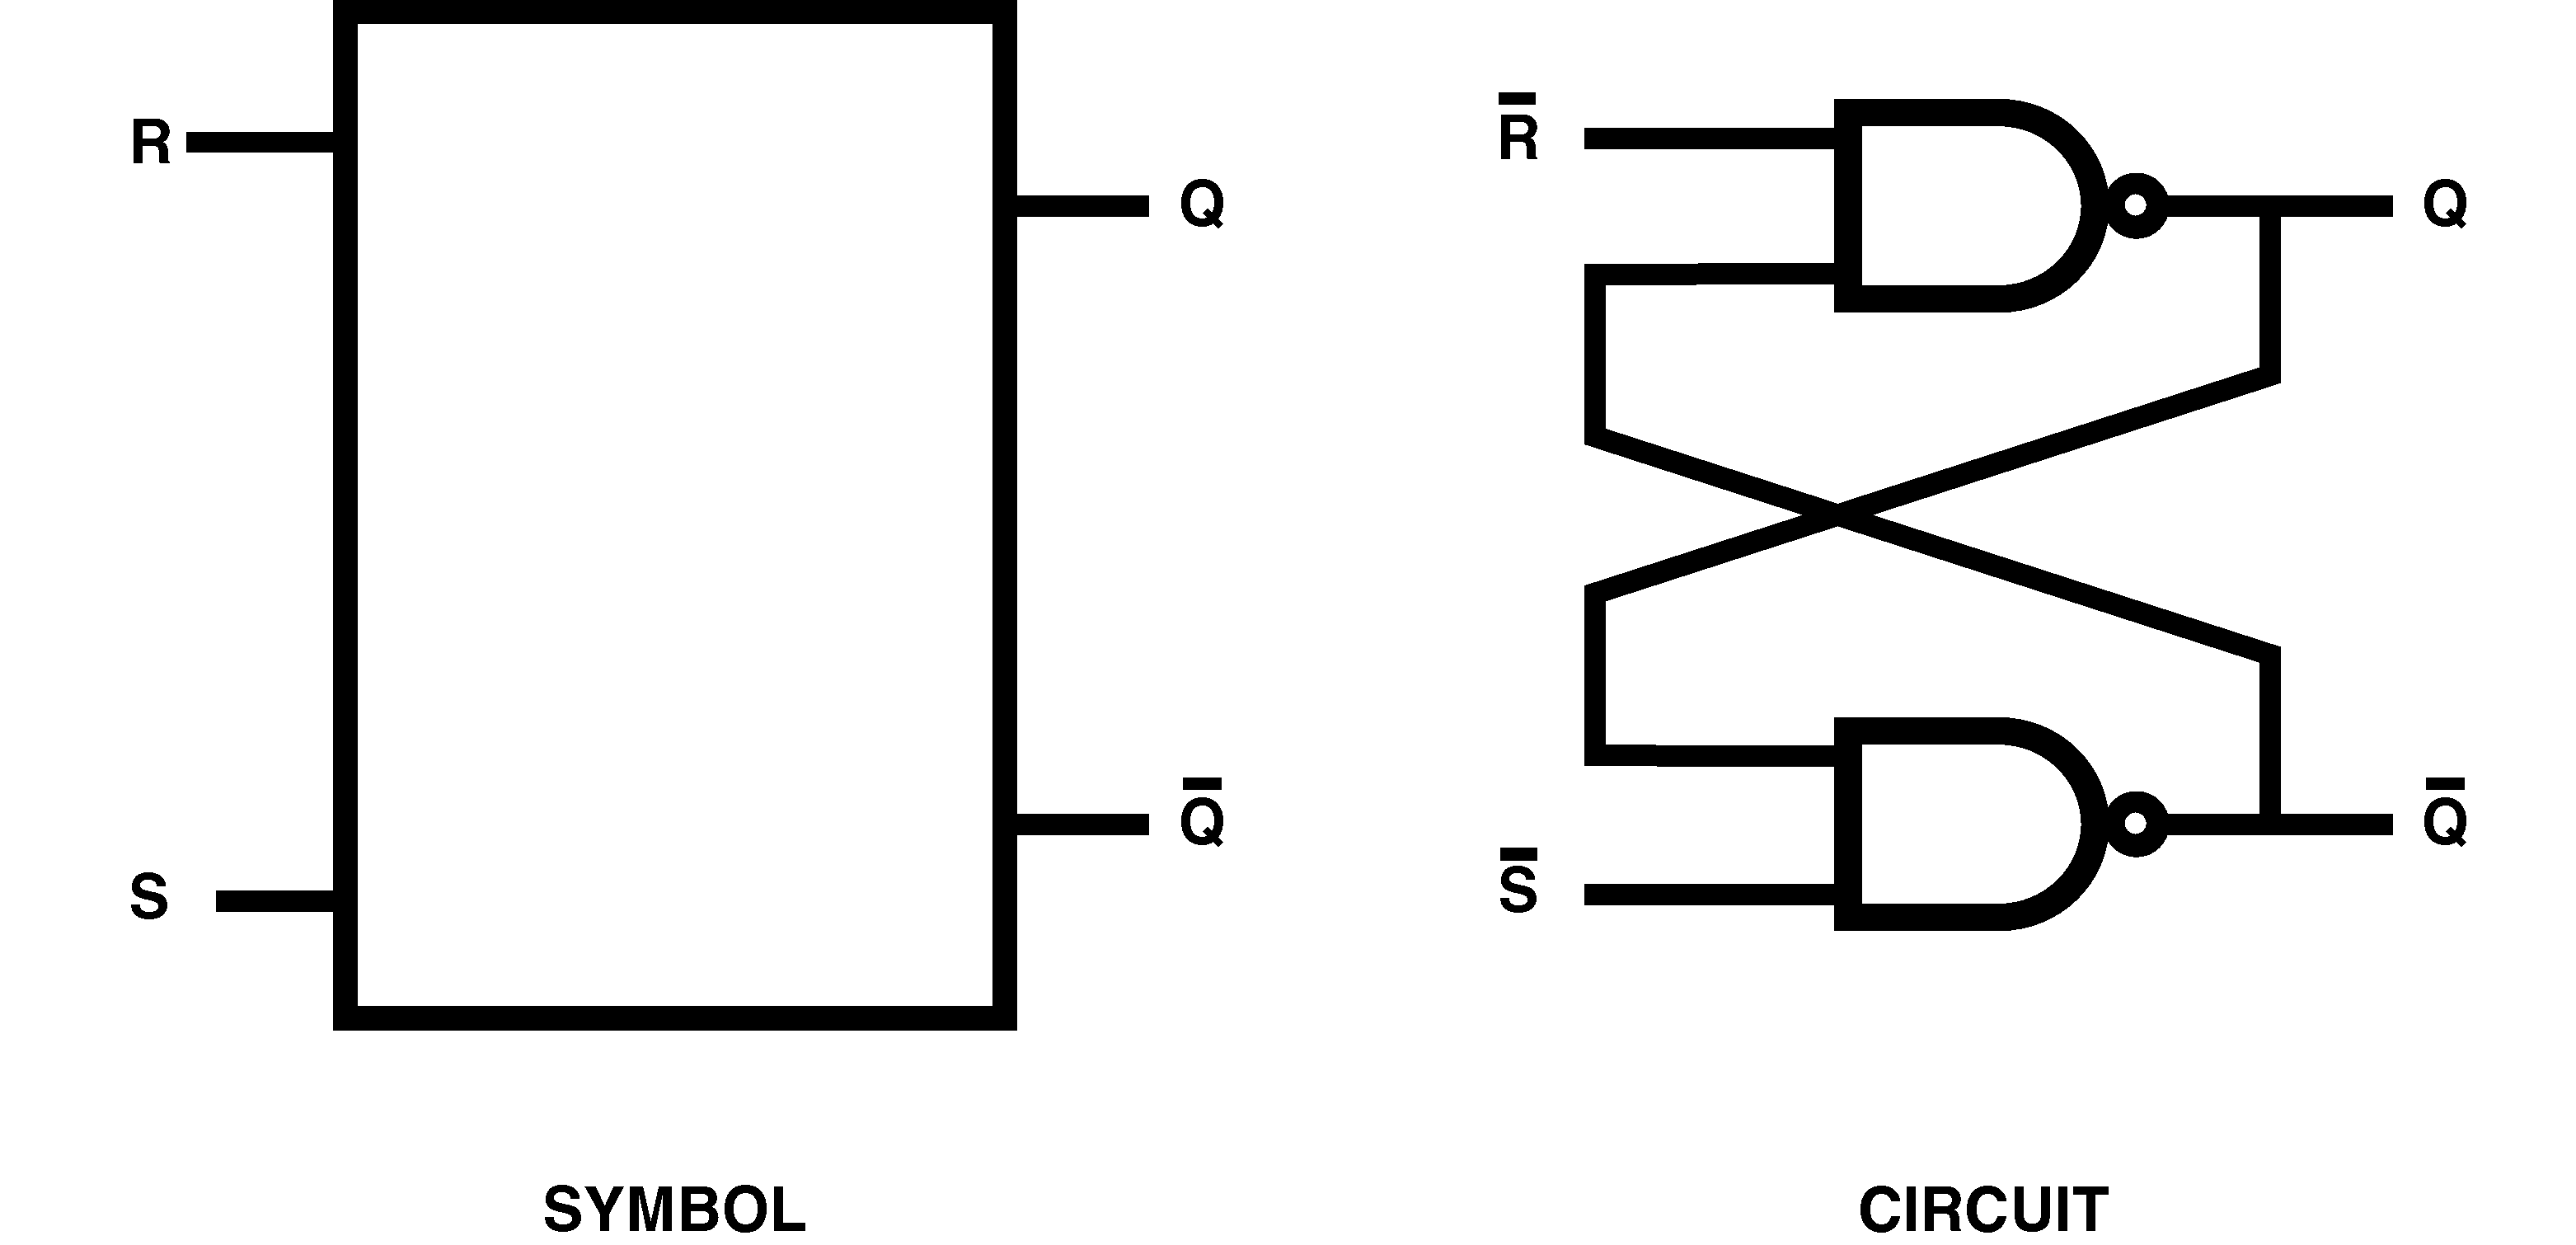
\includegraphics[width=0.95\linewidth]{images/5_memory/flip_flop_sr_nand.pdf}
		\caption{Il flip-flop SR: vedi il \underline{\href{https://www.youtube.com/watch?v=Y9k2oiSJkz4}{video su youtube}}}
	\end{figure}
	
\end{frame}


\subsubsection[Flip-flop D]{Flip-flop D}
\begin{frame}
	\frametitle{Flip-flop D}
	 
	\begin{figure}[!htbp] 
		\centering
		%\advance\leftskip-0.25cm
		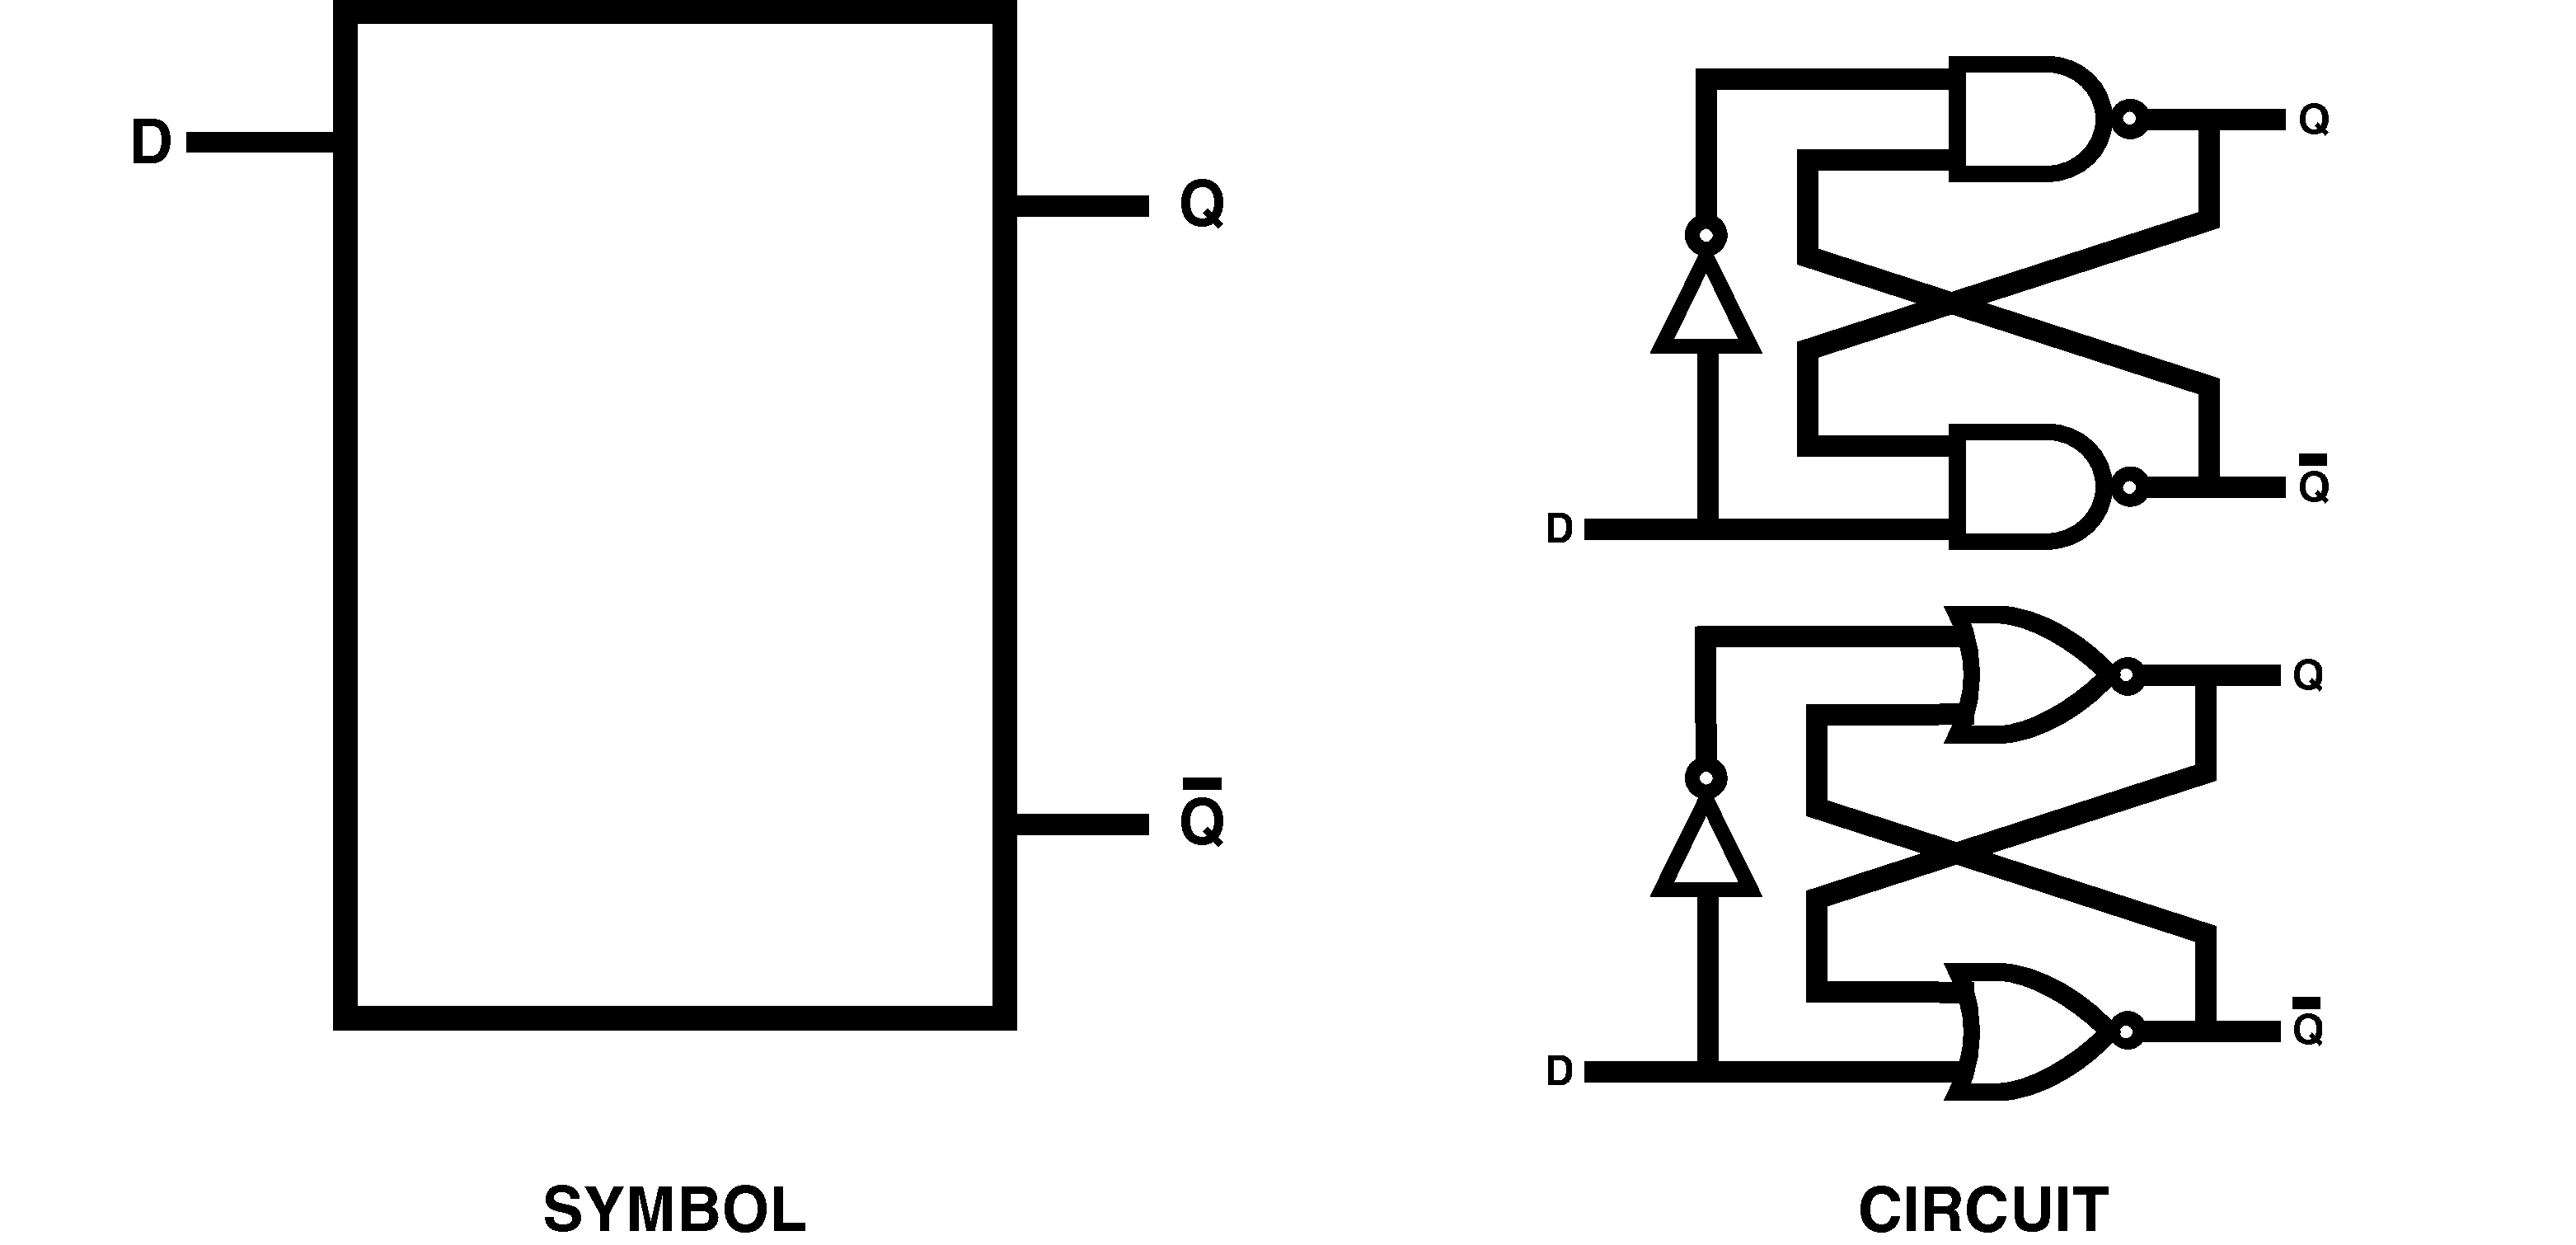
\includegraphics[width=0.75\linewidth]{images/5_memory/flip_flop_d.pdf}
		\caption{Il flip-flop D: è utile per memorizzare un bit di informazione che vengono presentate su una sola line detta "\textbf{Data Line}" (da cui la lettera \textbf{D})}
	\end{figure}
	
\end{frame}




\subsection[La ROM (Read Only Memory)]{La ROM (Read Only Memory)}
\begin{frame}
	\frametitle{La ROM: Read Only Memory}
	  
	\begin{block}{}
		In elettronica e informatica, una memoria di sola lettura, meglio nota come \textbf{ROM (Read Only Memory)}, indica un tipo di memoria \textit{non volatile} in cui i dati sono memorizzati tramite collegamenti elettronici fisici e stabili.
		
		\begin{figure}[!htbp] 
			\centering
			%\advance\leftskip-0.25cm
			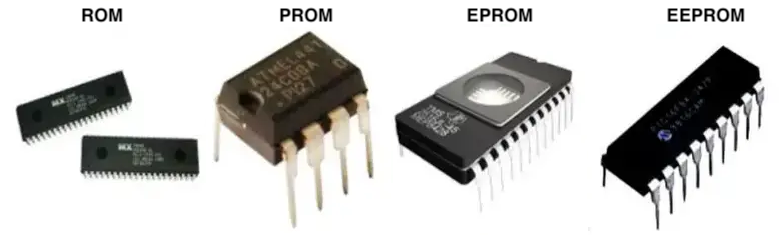
\includegraphics[width=0.80\linewidth]{images/5_memory/roms.png}
			%\caption{Il flip-flop D: è utile per memorizzare un bit di informazione che vengono presentate su una sola line detta "\textbf{Data Line}" (da cui la lettera \textbf{D})}
		\end{figure}
		
		Nonostante il nome suggerisca diversamente alcune ROM possono essere riscritte se sottoposte a specifiche condizioni fisiche.
		
		
		%Contrariamente alla maggior parte delle unità di memoria di massa il suo contenuto non è modificabile durante il normale funzionamento, ma può esserlo, con diverse tecniche, in fase di progettazione, prototipazione o costruzione.
	\end{block}
	
\end{frame}


\subsubsection[Le tipologie di ROM]{Le tipologie di ROM}
\begin{frame}
	\frametitle{Le tipologie di ROM}
	  
	\begin{block}{}
		
		Ogni tipo di ROM è programmata in modo differente a seconda del suo tipo e richiede condizioni speciali per essere cancellata o riscritta.
		
		\begin{figure}[!htbp] 
			\centering
			%\advance\leftskip-0.25cm
			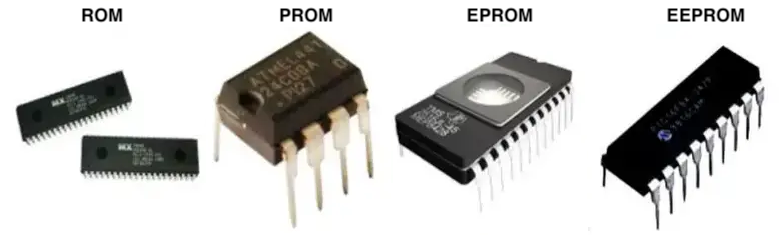
\includegraphics[width=0.80\linewidth]{images/5_memory/roms.png}
			%\caption{Il flip-flop D: è utile per memorizzare un bit di informazione che vengono presentate su una sola line detta "\textbf{Data Line}" (da cui la lettera \textbf{D})}
		\end{figure}
		
		Le  memorie ROM vengono in genere utilizzate per memorizzare programmi e dati di configurazione essenziali per il funzionamento del computer che devono essere memorizzati anche quando il computer è spento.
	\end{block}
	
\end{frame}


\subsubsection[ROM non programmabili]{ROM non programmabili}
\begin{frame}
	\frametitle{Le tipologie di ROM: non programmabili}
	  
	\begin{block}{}
		
		\begin{enumerate}
			\item \textbf{ROM non programmabili}: ROM a maschera, il cui nome deriva dal processo di litografia utilizzato nei circuiti integrati (chip), in cui una fotomaschera permette la creazione del chip. Vengono prodotte già con il programma o i dati "stampati" al loro interno.
		\end{enumerate}
	\end{block}
	
	\begin{columns}			
		\column{0.5\linewidth}
		\begin{figure}[!htbp]
			\centering 
			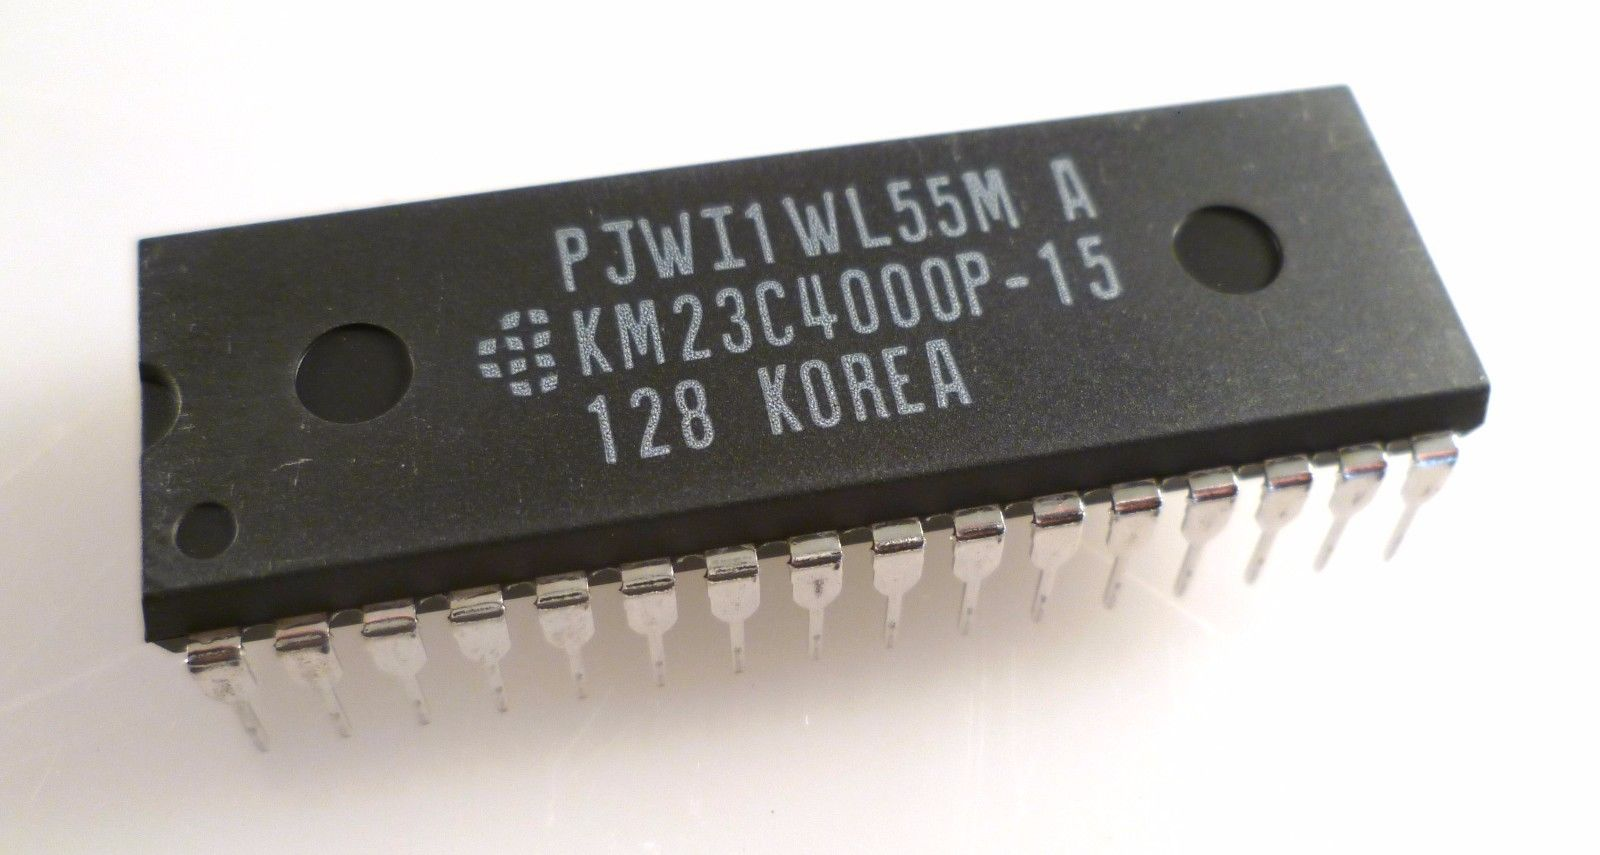
\includegraphics[width=1.0\linewidth]{images/5_memory/rom_mask_top.jpeg}
%				\caption{ROM a maschera}
		\end{figure}
		
		\column{0.5\linewidth}
		\begin{figure}[!htbp]
			\centering 
			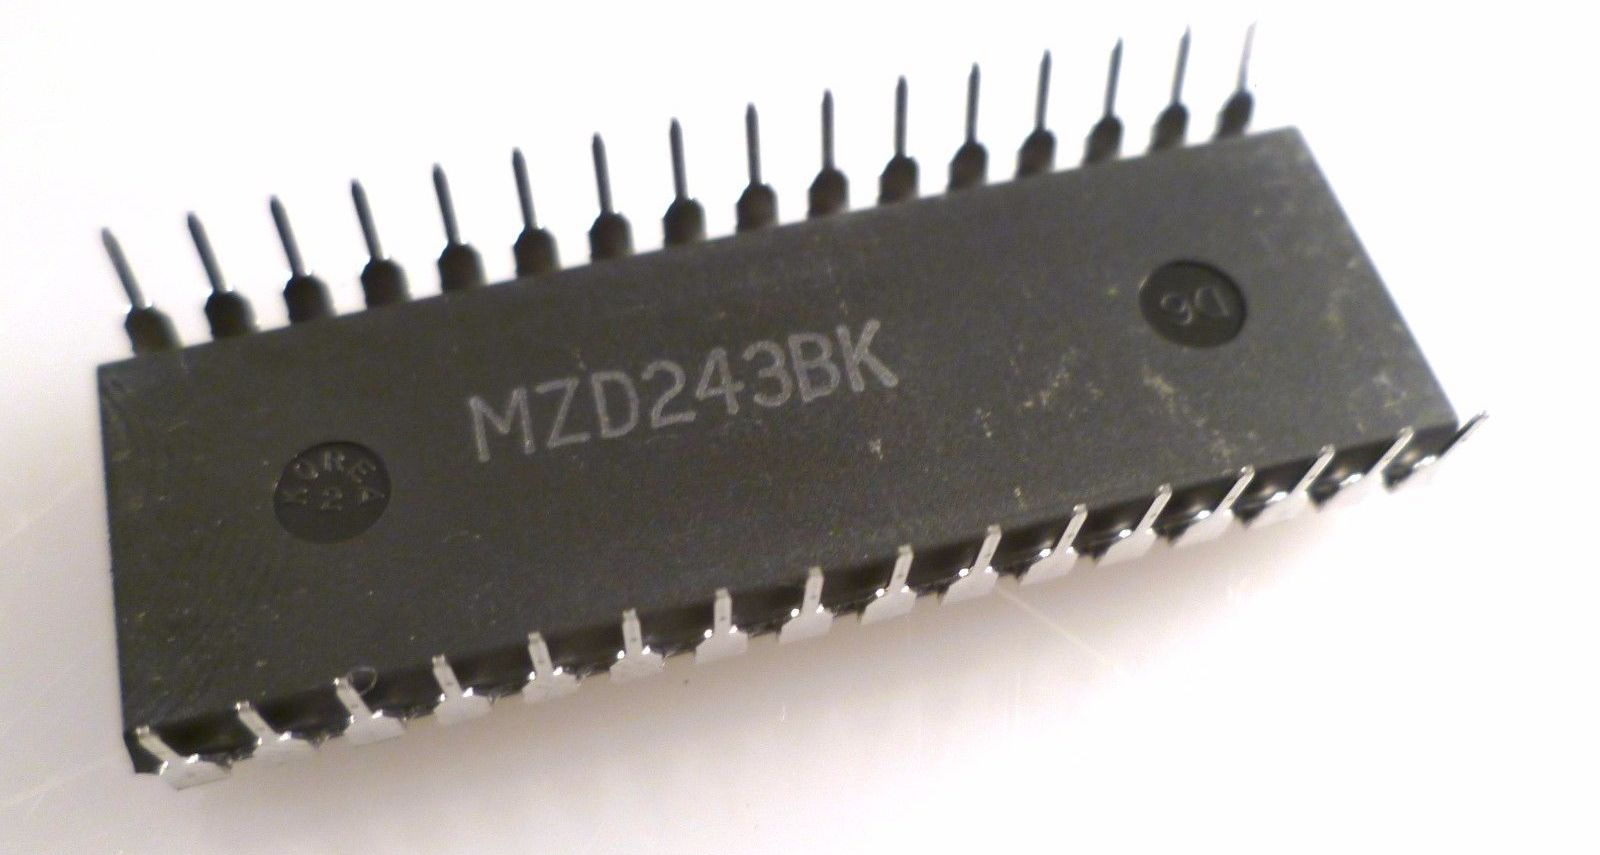
\includegraphics[width=1.0\linewidth]{images/5_memory/rom_mask_bottom.jpeg}
%				\caption{PCI Express: x16, x1, x4, x16} 
		\end{figure}
	\end{columns}
	
\end{frame}


\subsubsection[PROM  (Programmable  ROM)]{PROM  (Programmable  ROM)}
\begin{frame}
	\frametitle{Le tipologie di ROM: PROM}
	  
	\begin{block}{}
		
		\begin{enumerate}
			\setcounter{enumi}{1}
			\item \textbf{PROM  (Programmable  ROM)}: normalmente vengono prodotte vuote al loro interno, possono essere programmate successivamente attraverso appositi \textbf{programmatori di PROM},  tuttavia, una volta programmate, non possono essere più modificate nel  contenuto.
		\end{enumerate}
	\end{block}
	
	\begin{figure}[!htbp] 
		\centering
		%\advance\leftskip-0.25cm
		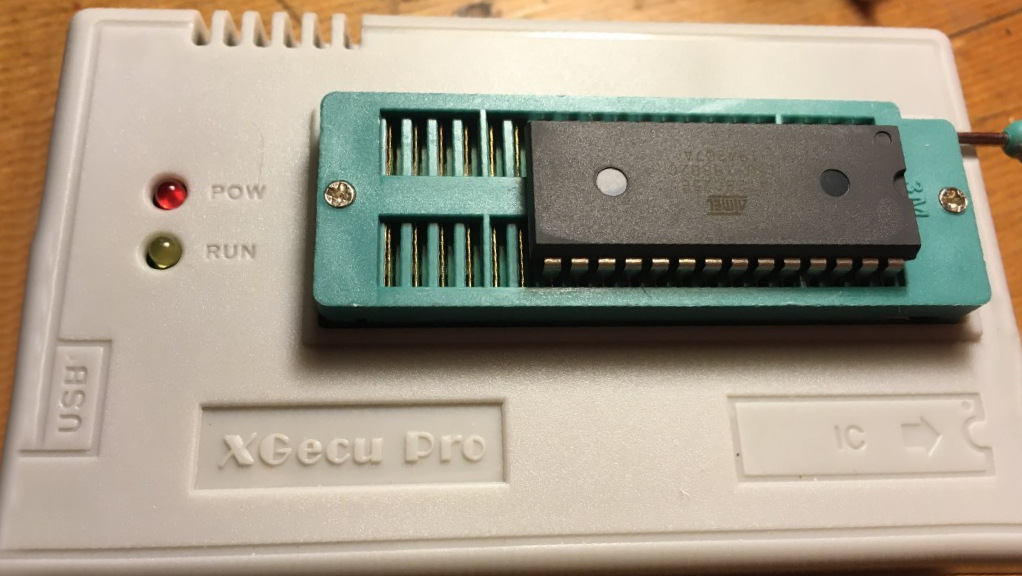
\includegraphics[width=0.7\linewidth]{images/5_memory/prom_programmer.png}
		%\caption{Programmatore di PROM}
	\end{figure}
	
\end{frame}


\subsubsection[EPROM (Erasable Programmable ROM)]{EPROM (Erasable Programmable ROM)}
\begin{frame}
	\frametitle{Le tipologie di ROM: EPROM}
	  
	\begin{block}{}

		\begin{enumerate}
			\setcounter{enumi}{2}
			\item \textbf{EPROM (Erasable Programmable ROM)}: normalmente sono vuote al loro interno e possono  essere  programmate  attraverso appositi programmatori di EPROM. A differenza delle PROM, la programmazione può avvenire più volte, a patto di cancellare la vecchia programmazione tramite raggi UV (ultravioletti).
		\end{enumerate}
		
	\end{block}
	
	\begin{columns}			
		\column{0.5\linewidth}
		\begin{figure}[!htbp]
			\centering 
			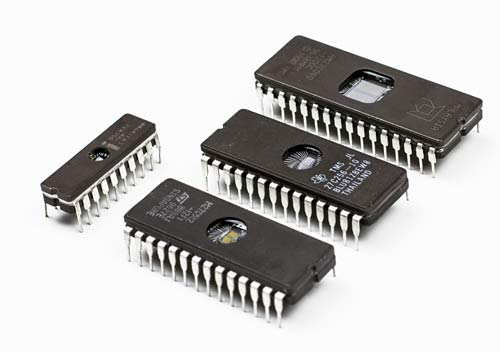
\includegraphics[width=1.0\linewidth]{images/5_memory/eproms.jpg }
%				\caption{ROM a maschera}
		\end{figure}
		
		\column{0.5\linewidth}
		\begin{figure}[!htbp]
			\centering 
			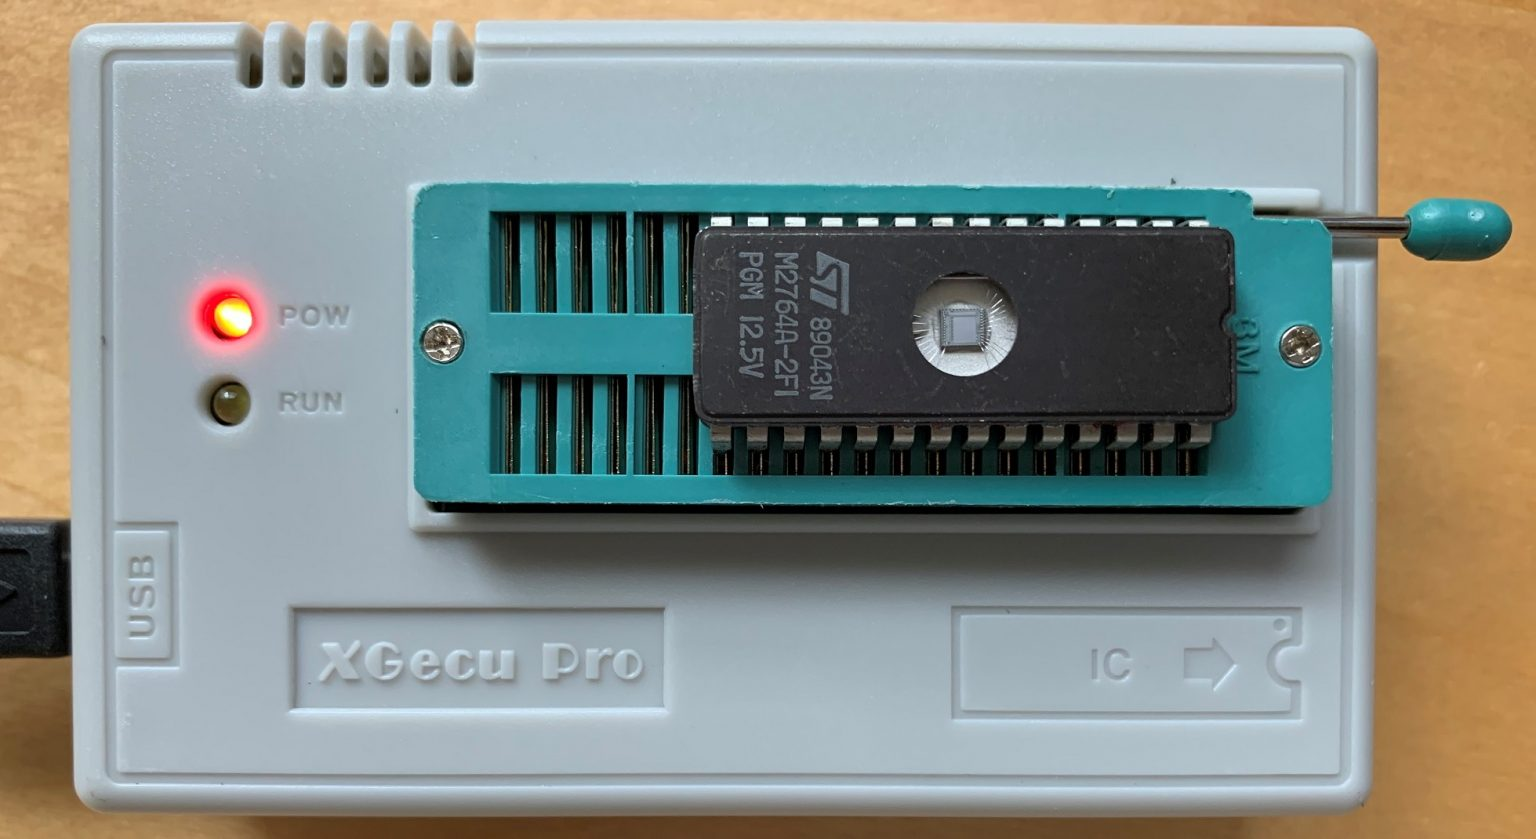
\includegraphics[width=1.0\linewidth]{images/5_memory/eprom_programmer.jpg}
%				\caption{PCI Express: x16, x1, x4, x16} 
		\end{figure}
	\end{columns}
	
	\begin{figure}[!htbp] 
		\centering
		%\advance\leftskip-0.25cm
		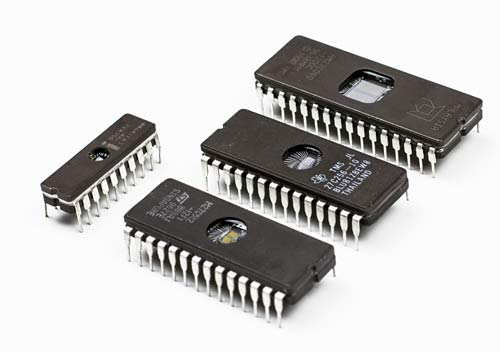
\includegraphics[width=0.5\linewidth]{images/5_memory/eproms.jpg }
		%\caption{PROM: nota la finestrella posta nella parte superiore del  circuito, che permette di ricevere i raggi UV}
	\end{figure}
	
\end{frame}



\begin{frame}
	\frametitle{Le tipologie di ROM: EPROM}
	 
	\begin{figure}[!htbp] 
		\centering
		%\advance\leftskip-0.25cm
		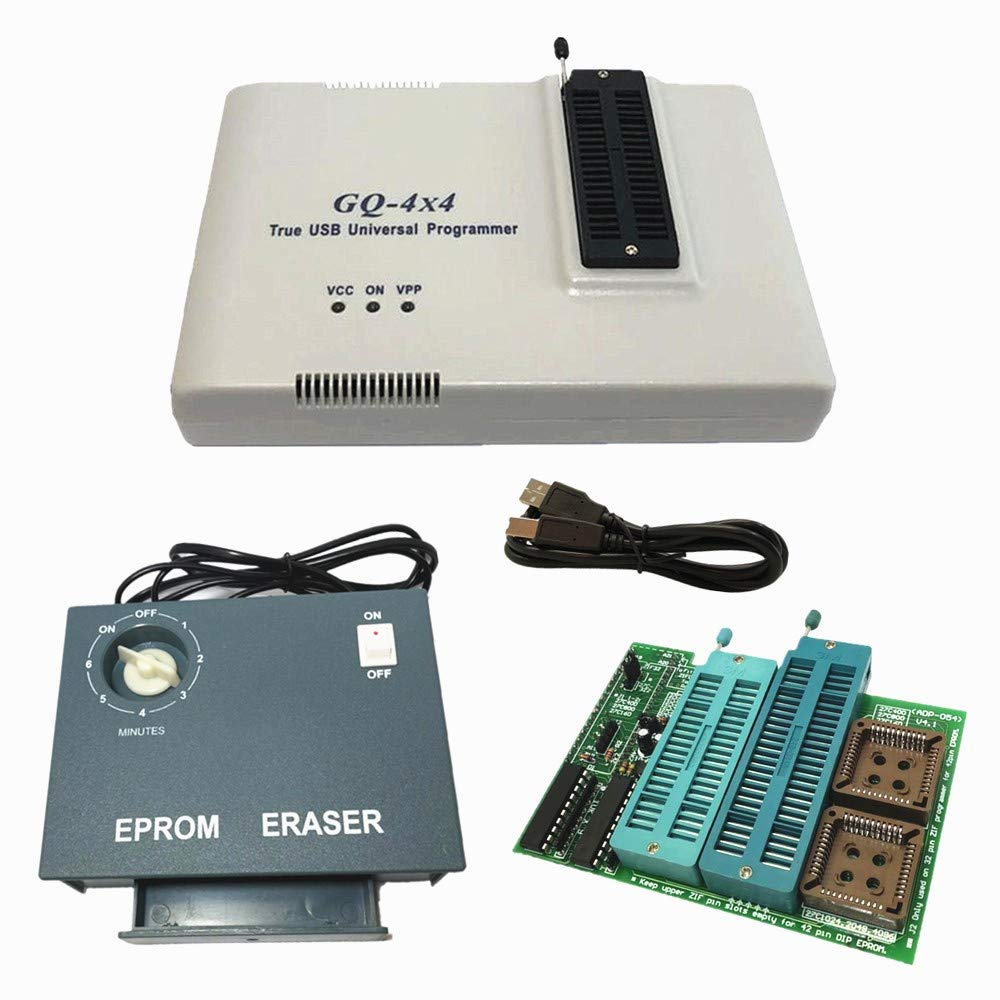
\includegraphics[width=0.6\linewidth]{images/5_memory/eprom_writer_eraser.jpg}
		%\caption{PROM: nota la finestrella posta nella parte superiore del  circuito, che permette di ricevere i raggi UV}
	\end{figure}
	
\end{frame}


\begin{frame}
	\frametitle{Le tipologie di ROM: EPROM}
	 
	\begin{figure}[!htbp] 
		\centering
		%\advance\leftskip-0.25cm
		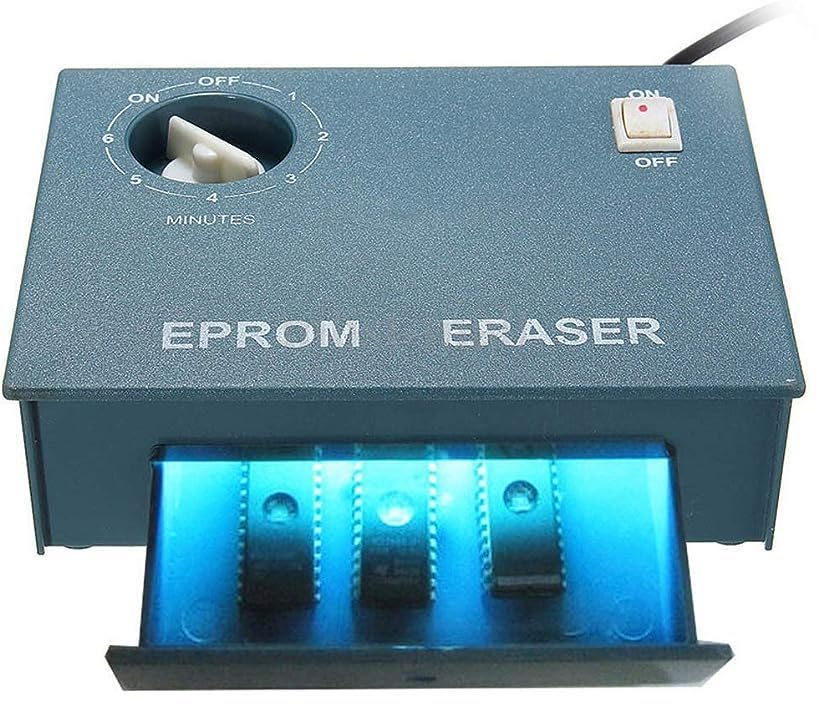
\includegraphics[width=0.6\linewidth]{images/5_memory/eprom_eraser.jpg}
		%\caption{PROM: nota la finestrella posta nella parte superiore del  circuito, che permette di ricevere i raggi UV}
	\end{figure}
	
\end{frame}



\subsubsection[EEPROM (Electrical  Erasable  Programmable  ROM)]{EEPROM (Electrical  Erasable  Programmable  ROM)}
\begin{frame}
	\frametitle{Le tipologie di ROM: EEPROM}
	  
	\begin{block}{}

		\begin{enumerate}
			\setcounter{enumi}{3}
			\item \textbf{EEPROM (Electrical  Erasable  Programmable  ROM)}: identiche alle EPROM, dalle quali differiscono solo per il fatto che la cancellazione della vecchia programmazione è realizzata più semplicemente tramite un flusso di corrente elettrica. 
		\end{enumerate}
		
	\end{block}
	
	\begin{figure}[!htbp] 
		\centering
		%\advance\leftskip-0.25cm
		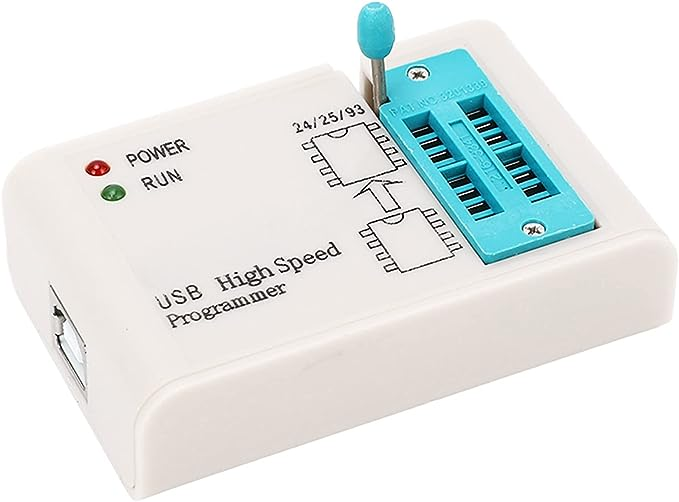
\includegraphics[width=0.55\linewidth]{images/5_memory/eeprom_programmer.jpg}
		%\caption{Programmatore di PROM}
	\end{figure}
	
\end{frame}




\subsection[La RAM (Random Access Memory)]{La RAM (Random Access Memory)}
\begin{frame}
	\frametitle{La RAM (Random Access Memory)}
	  
	\begin{block}{}
		La \textbf{memoria ad accesso casuale} o \textbf{RAM} (Random Access Memory), è un tipo di memoria volatile caratterizzata dal permettere l'accesso diretto a qualunque indirizzo di memoria con le stesse identiche tempistiche.
		
		\begin{figure}[!htbp]
			\centering
			%\advance\leftskip-0.25cm
			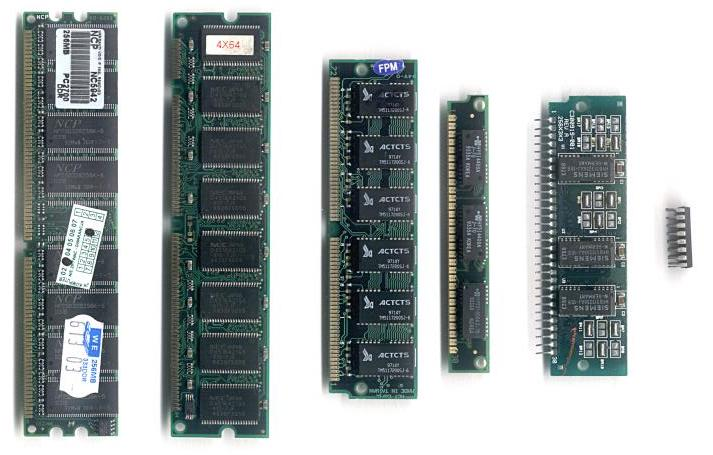
\includegraphics[width=0.58\linewidth]{images/5_memory/ram.jpg}
%			\caption{RAM (Random Access Memory)}
			\label{fig:memory_ram}
		\end{figure}
	\end{block}
\end{frame}



% http://www.brescianet.com/appunti/infobase/pc_C.htm
\subsubsection[I tipi di RAM]{I tipi di RAM}
\begin{frame}
	\frametitle{I tipi di RAM}
	  
	\begin{block}{}
		%La RAM si contrappone alla memoria ad accesso sequenziale, in cui i dati sono disposti in modo sequenziale e per accedervi è necessario scorrere su tutti i dati precedenti.\\~\\
		
		Possiamo distinguere le RAM in diverse tipologie:
		\begin{itemize}
			\item Le \textbf{DRAM} (dynamic RAM): tempo di accesso 20-70ns con refresh. Sono \textbf{poco costose}. Sono principalmente utilizzate per la \textit{\underline{memoria centrale}} del computer.
			\item Le \textbf{SDRAM} (synchronous dynamic RAM): evoluzione della DRAM, sincrona rispetto al BUS di sistema, ovvero utilizza un segnale di clock esterno per la sincronizzazione delle operazioni di I/O; questo permette un incremento delle prestazioni e una maggiore efficienza.
			\item Le \textbf{SRAM} (static RAM): tempo di accesso 5-10ns senza refresh. Sono \textbf{rapide ma costose}. Sono soprattutto utilizzate per le \textit{\underline{memorie cache}} del processore.
			\item ... \textbf{FeRAM}, \textbf{memorie a cambiamento di fase} ...
			%\item Le \textbf{FeRAM} (ferroelectric dynamic RAM): mantiene i dati senza l'ausilio del refresh di sistema. Utilizzano un materiale denominato ferroelettrico che ha la capacità di mantenere la propria polarizzazione anche dopo esser scollegato dalla fonte energetica.
		\end{itemize}
	\end{block}
\end{frame}


\subsubsection[La DRAM: dynamic RAM]{La DRAM: dynamic RAM}
\begin{frame}
	\frametitle{La DRAM: dynamic RAM}
	  
	\begin{block}{}
		La memoria dinamica DRAM è costituita da centinaia di migliaia di piccoli \textbf{condensatori} (sorta di serbatoio elettrico) che immagazzinano delle cariche. Una volta caricato, lo stato software del condensatore è pari a 1, in caso contrario è a 0, il che significa che ogni condensatore rappresenta un bit della memoria.\\~\\
		Dato che i condensatori si scaricano, bisogna costantemente ricaricarli (il termine esatto è \textbf{refresh}) ad un intervallo di tempo regolare detto \textbf{ciclo di refresh}. Le memorie DRAM hanno ad esempio bisogno di cicli di refresh ogni 15 nanosecondi (ns) circa.\\~\\
		
		Oltre a comportare un certo dispendio di energia rendono più lenta la memoria in quanto, mentre si sta eseguendo il refreshing, non è possibile accedervi.
	\end{block}
\end{frame}

\begin{frame}
	\frametitle{La DRAM: dynamic RAM}
	  
	\begin{block}{}
		È importante sottolineare come l'operazione di lettura sia distruttiva, in quanto nel momento in cui un dato viene letto viene anche perso; risulta quindi necessaria la sua riscrittura immediata e questa porta a uno spreco di tempo.\\~\\
		Ogni condensatore è accoppiato ad un transistor (di tipo MOS) che permette di "recuperare" (leggere) o di modificare lo stato del condensatore. Questi transistor sono disposti sotto forma di tabella (matrice). I punti di memoria vengono indicati con una linea e una colonna.
	\end{block}
	
	\begin{columns}			
		\column{0.5\linewidth}
		\begin{figure}[!htbp]
			\centering 
			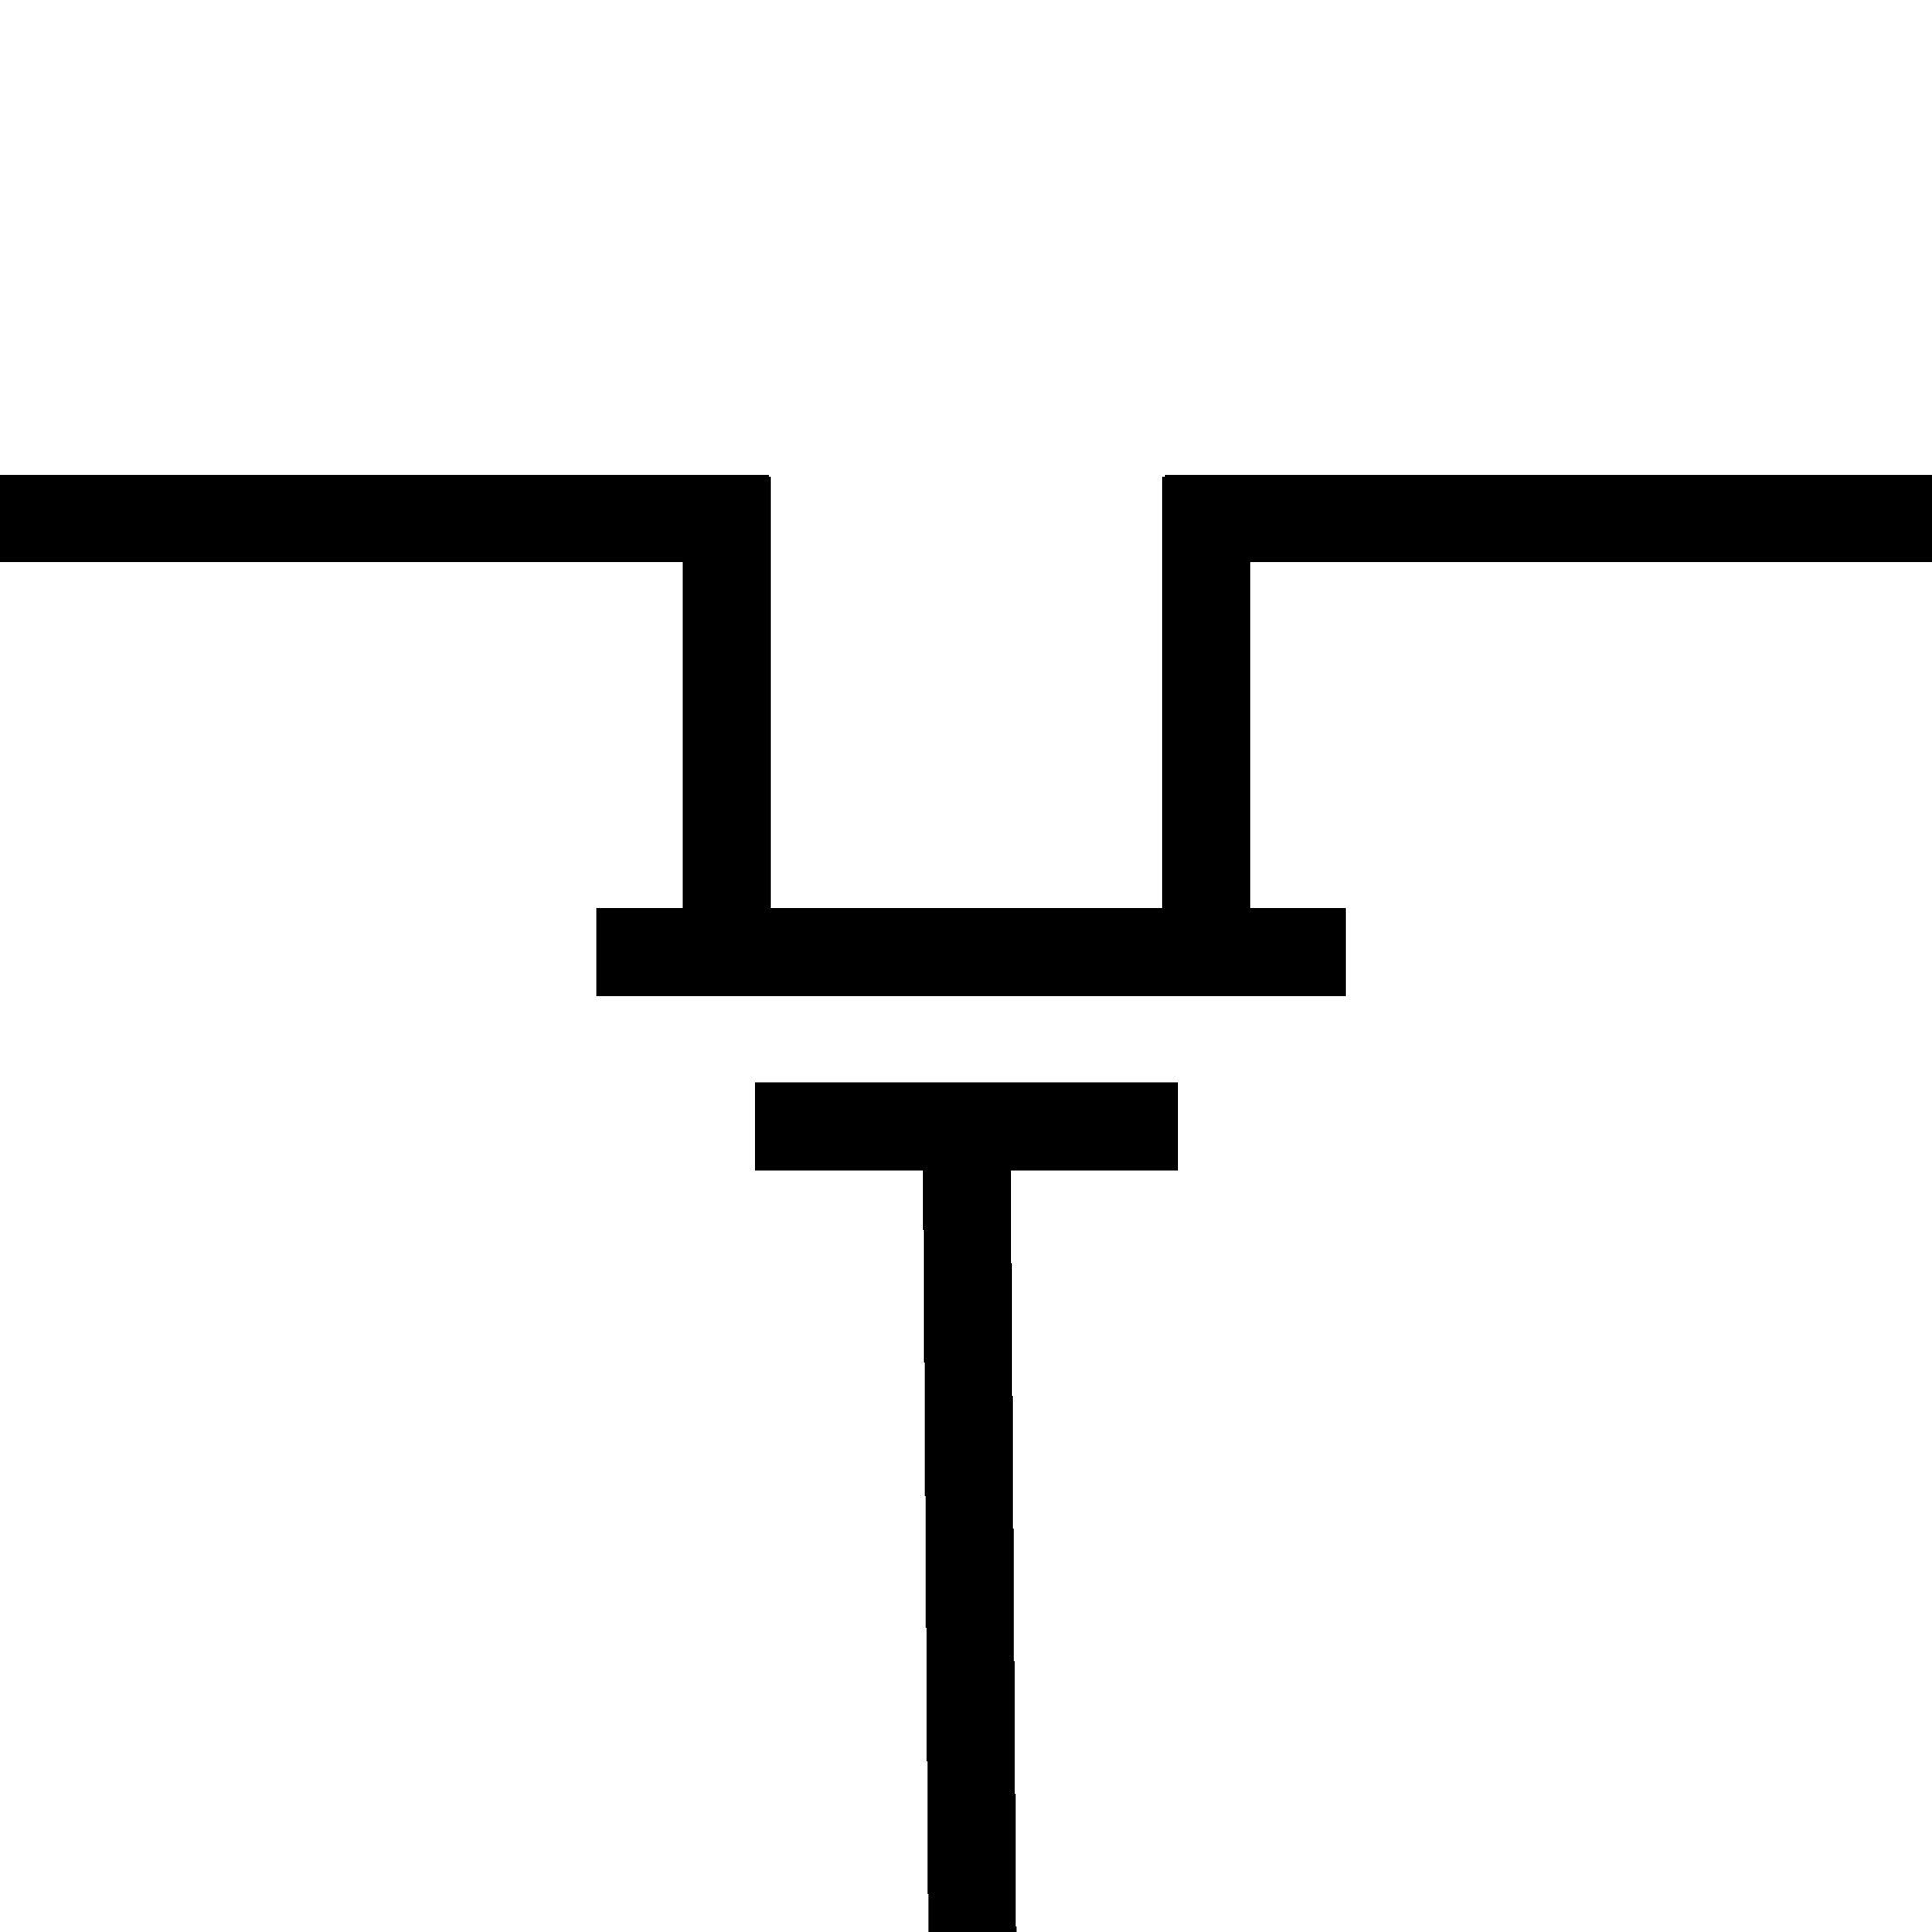
\includegraphics[width=0.15\linewidth]{images/5_memory/transistor.pdf}
				\caption{Transistor}
		\end{figure}
		
		\column{0.5\linewidth}
		\begin{figure}[!htbp]
			\centering 
			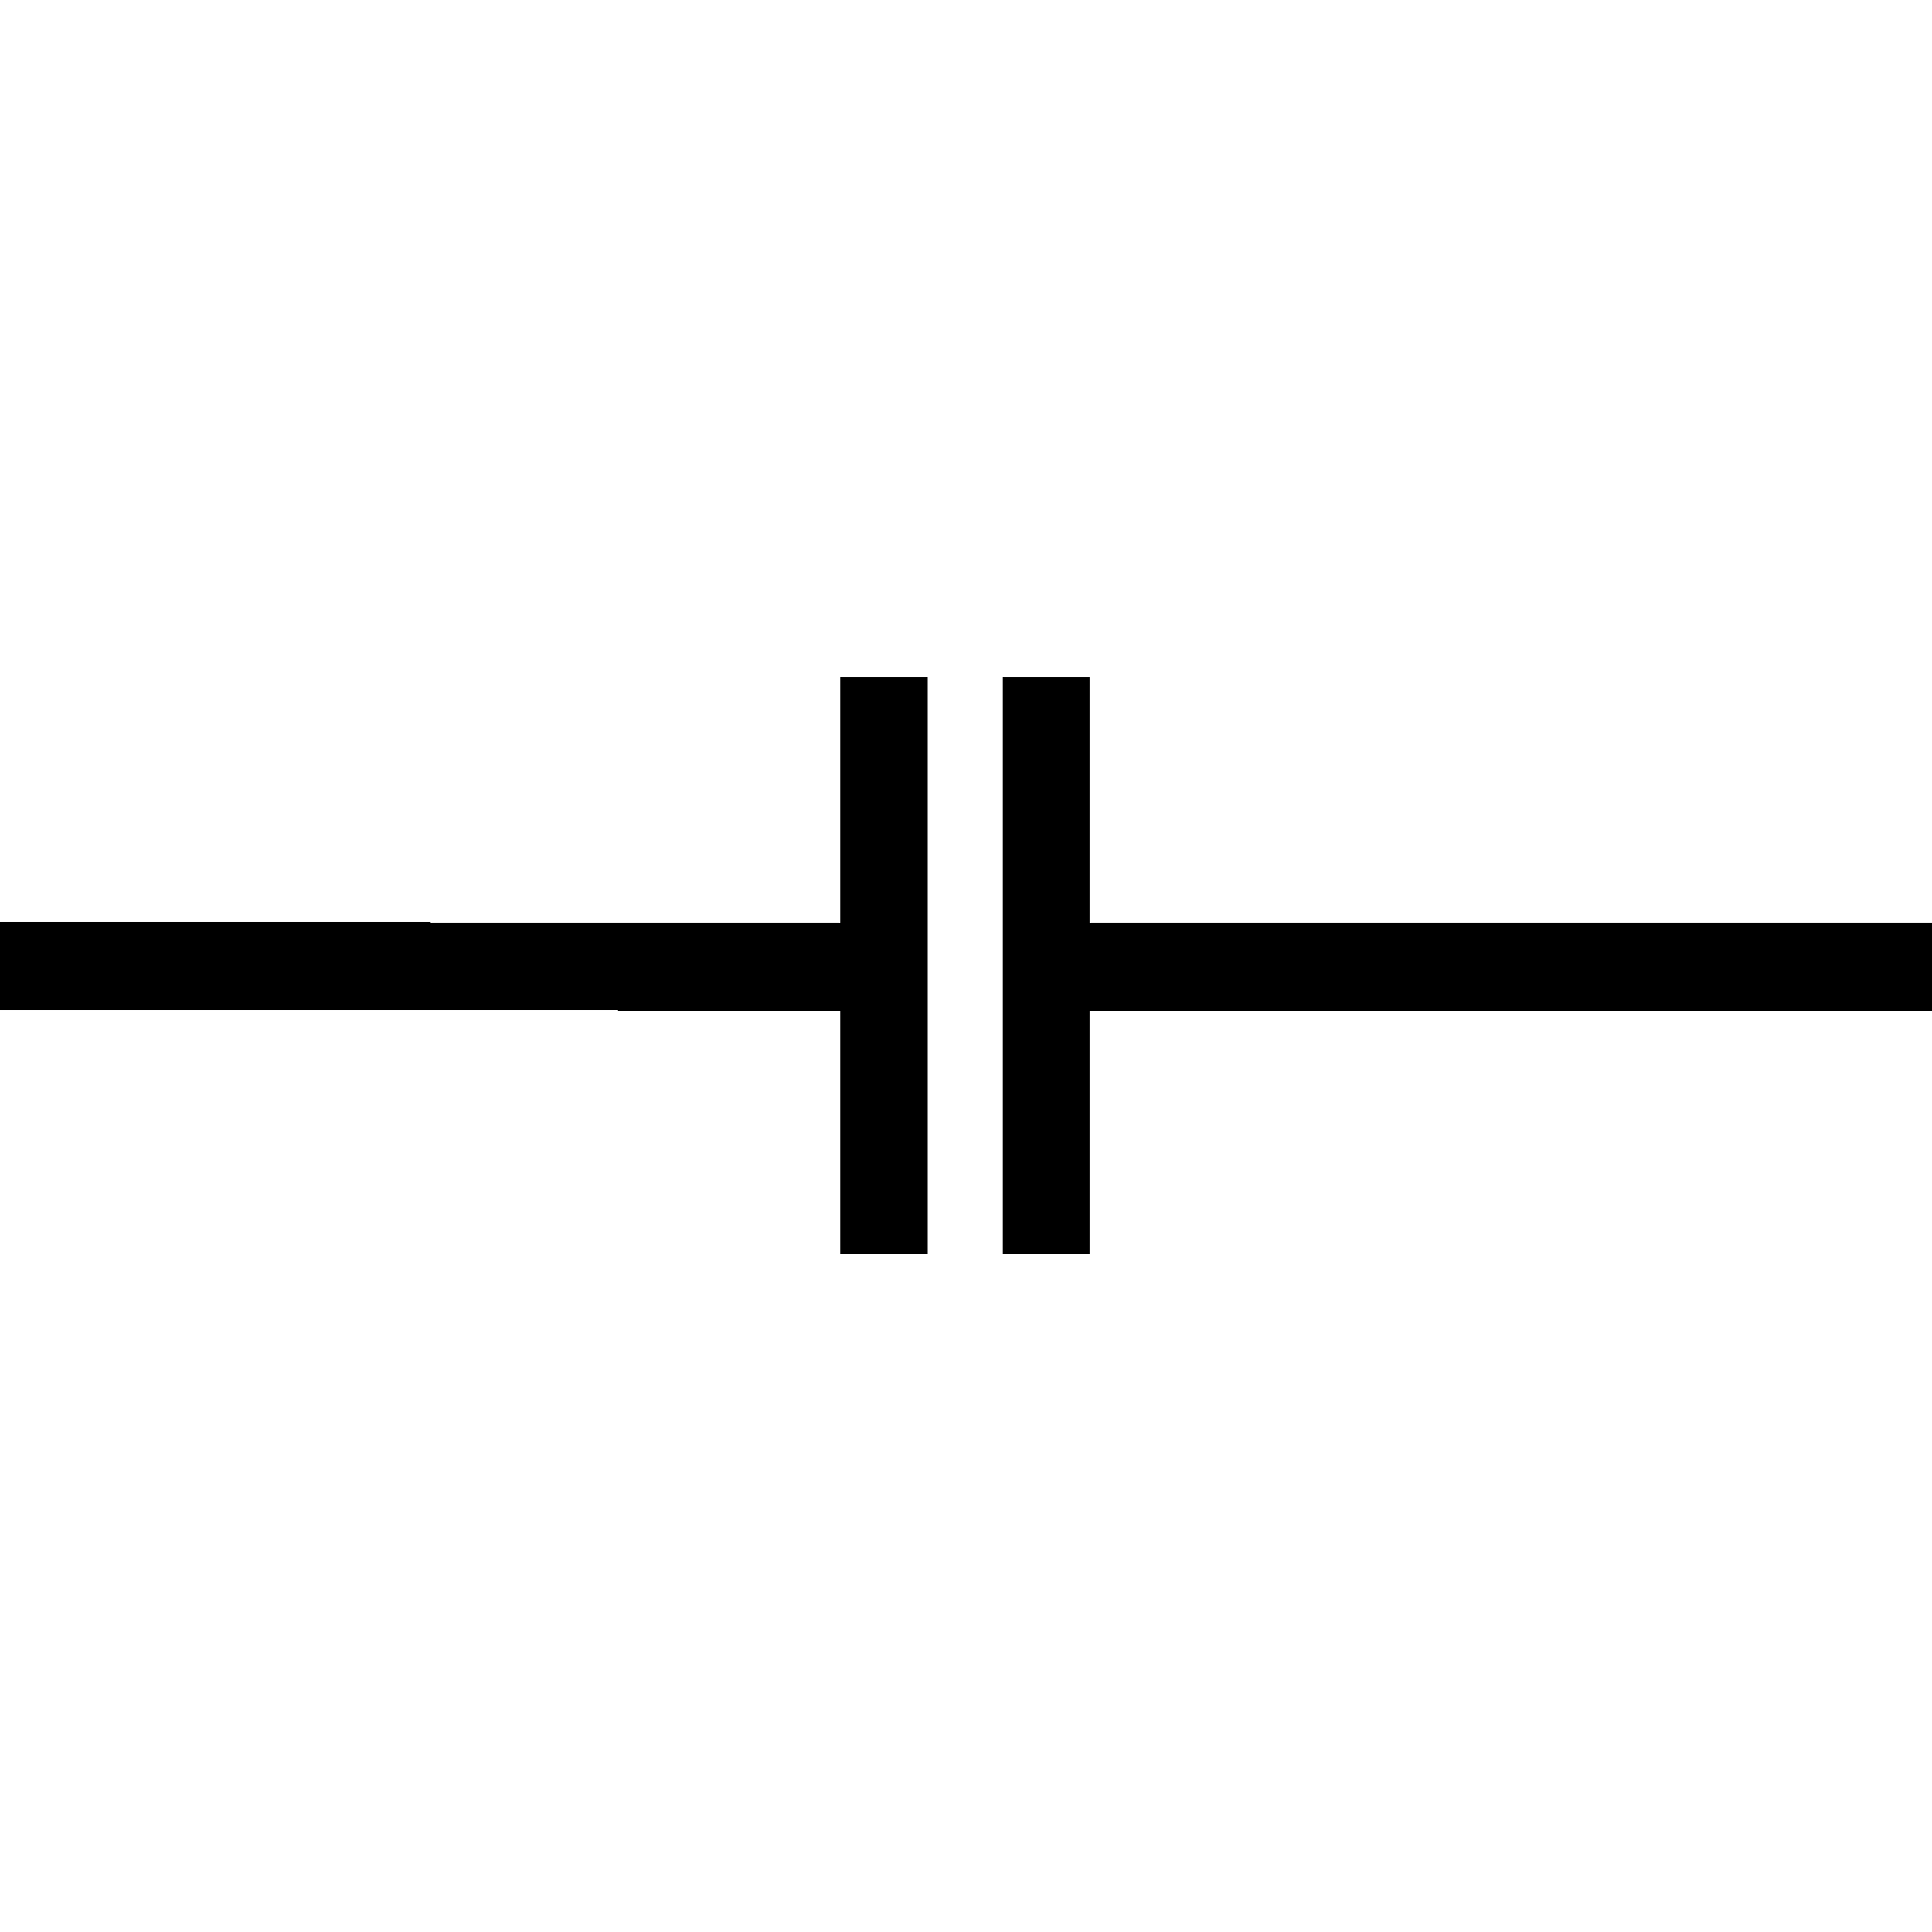
\includegraphics[width=0.15\linewidth]{images/5_memory/condensatore.pdf}
				\caption{Condensatore} 
		\end{figure}
	\end{columns}
\end{frame}


\begin{frame}
	\frametitle{La DRAM: dynamic RAM, }
	 
	\begin{figure}[!htbp] 
		\centering
		%\advance\leftskip-0.25cm
		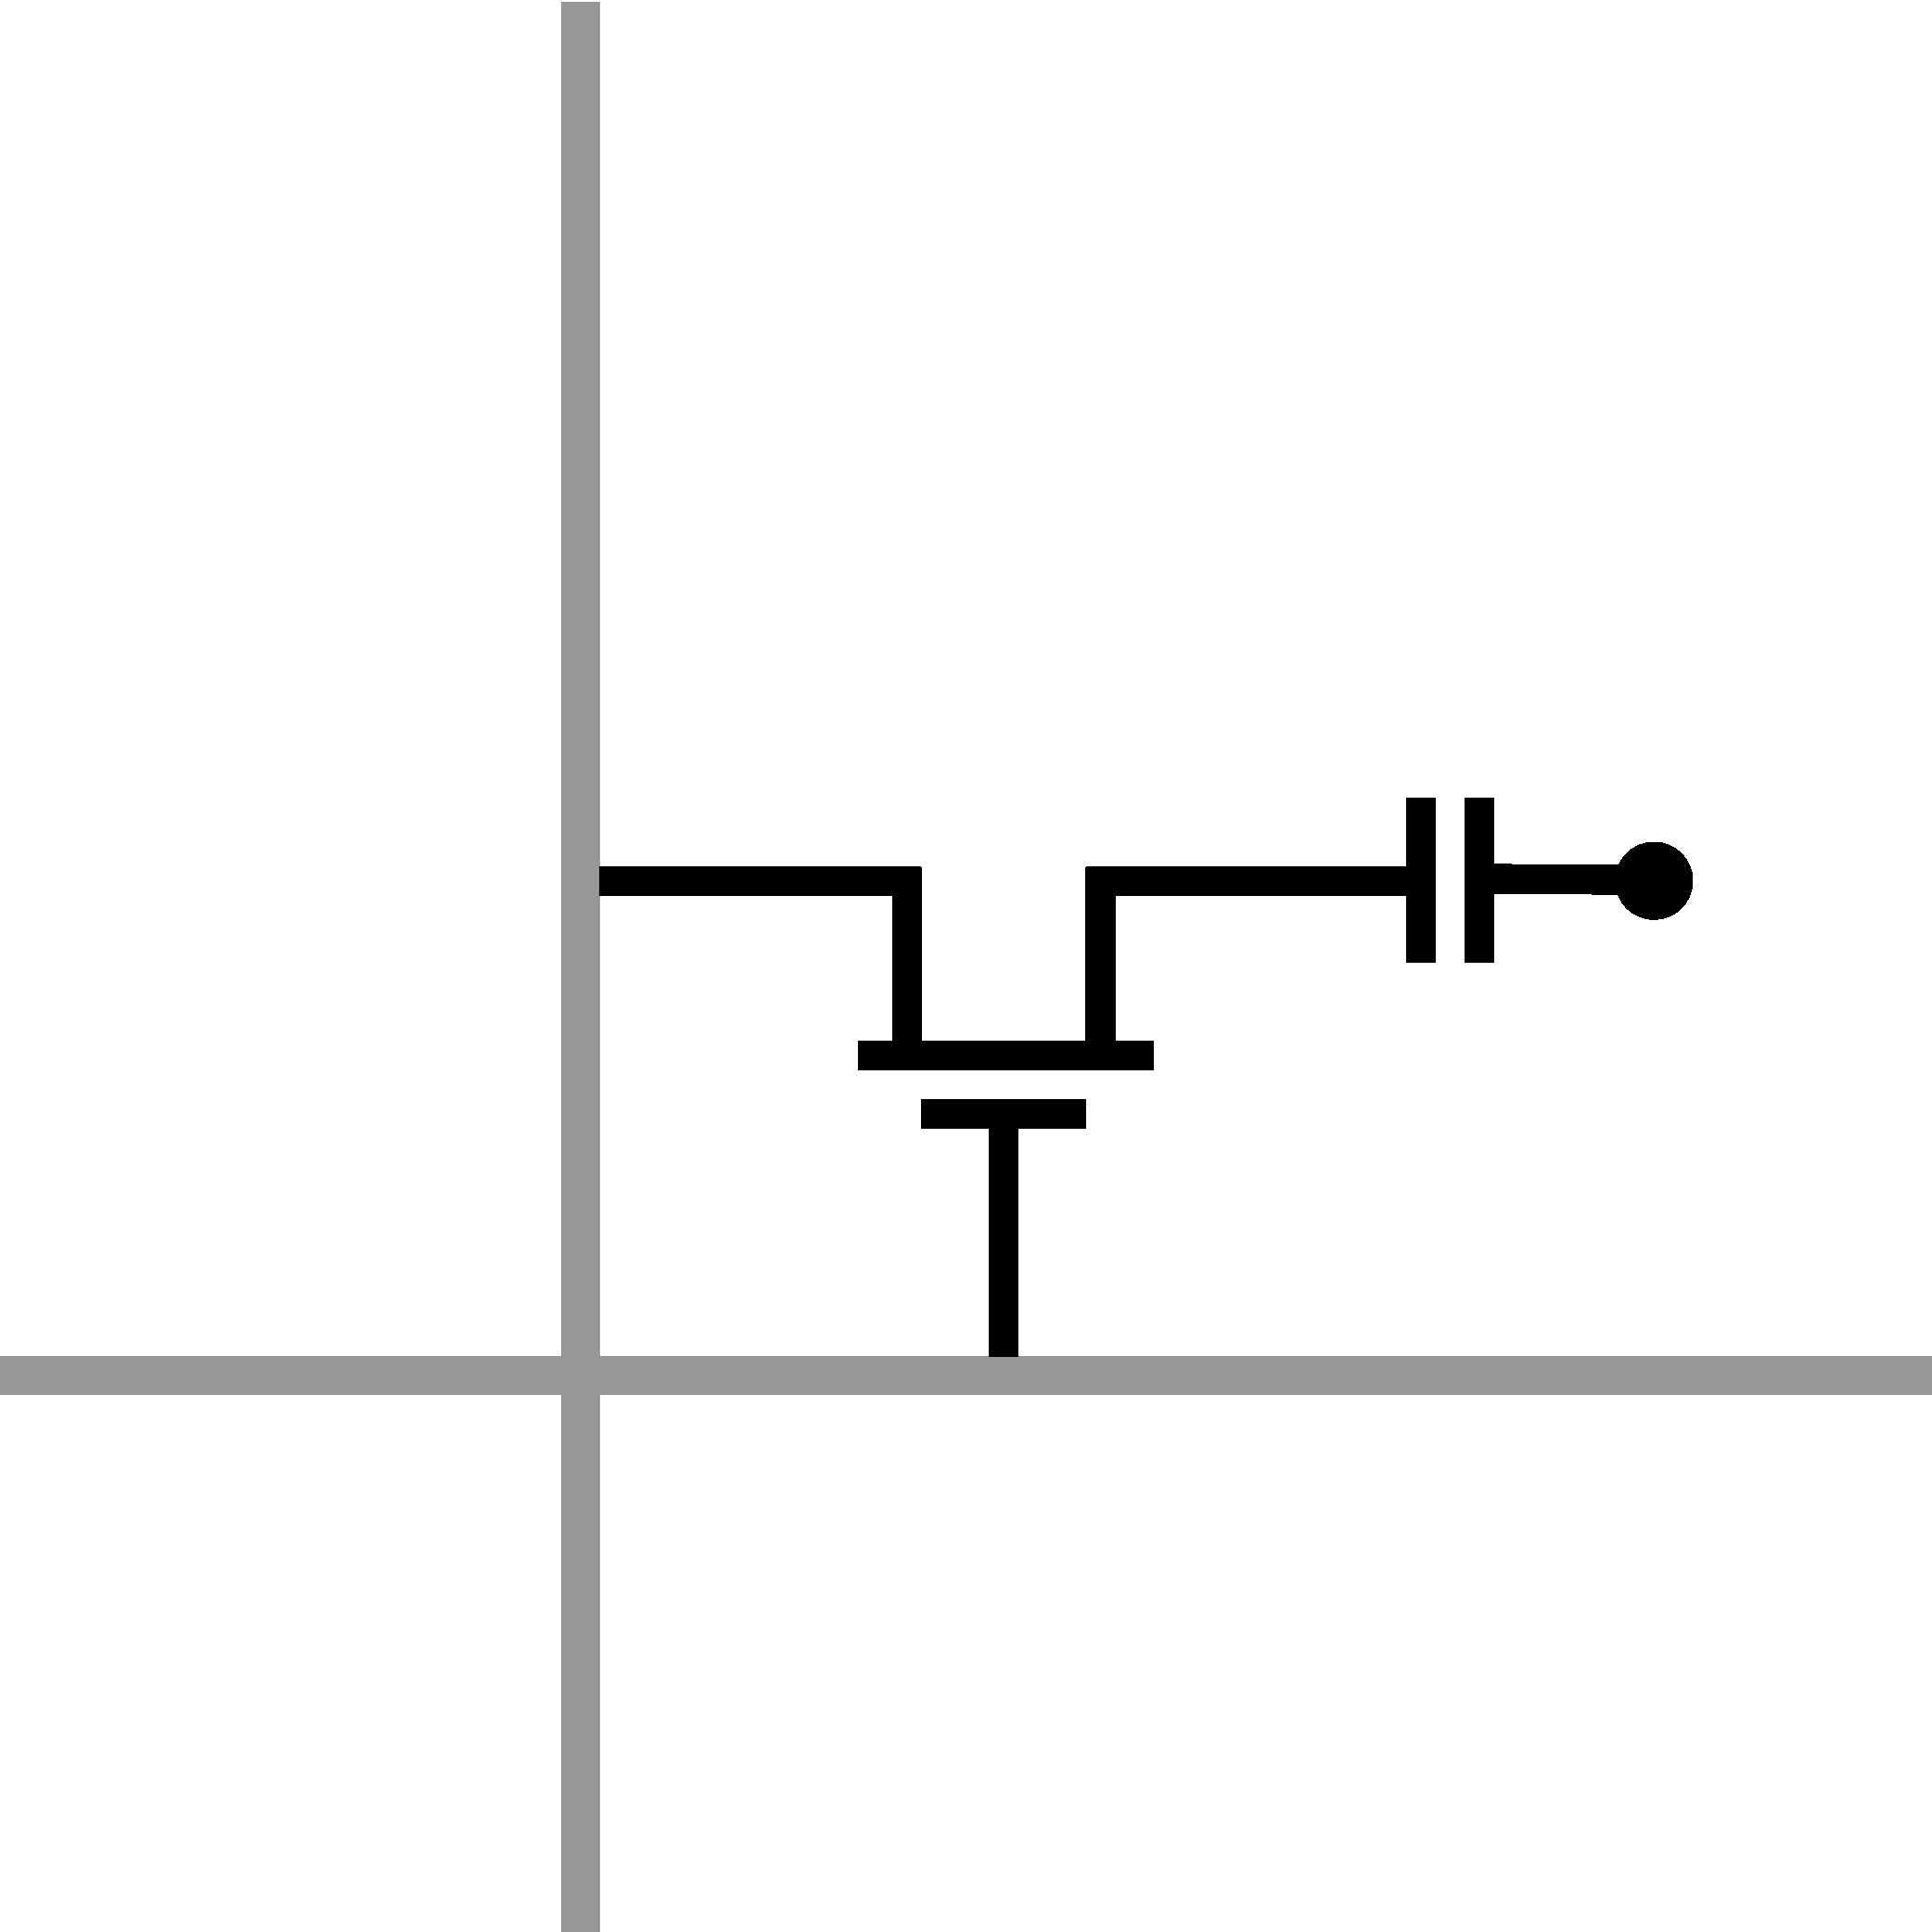
\includegraphics[width=0.6\linewidth]{images/5_memory/dram_bit.pdf}
		%\caption{PROM: nota la finestrella posta nella parte superiore del  circuito, che permette di ricevere i raggi UV}
	\end{figure}
	
\end{frame}


\begin{frame}
	\frametitle{La DRAM: dynamic RAM}
	 
	\begin{figure}[!htbp] 
		\centering
		%\advance\leftskip-0.25cm
		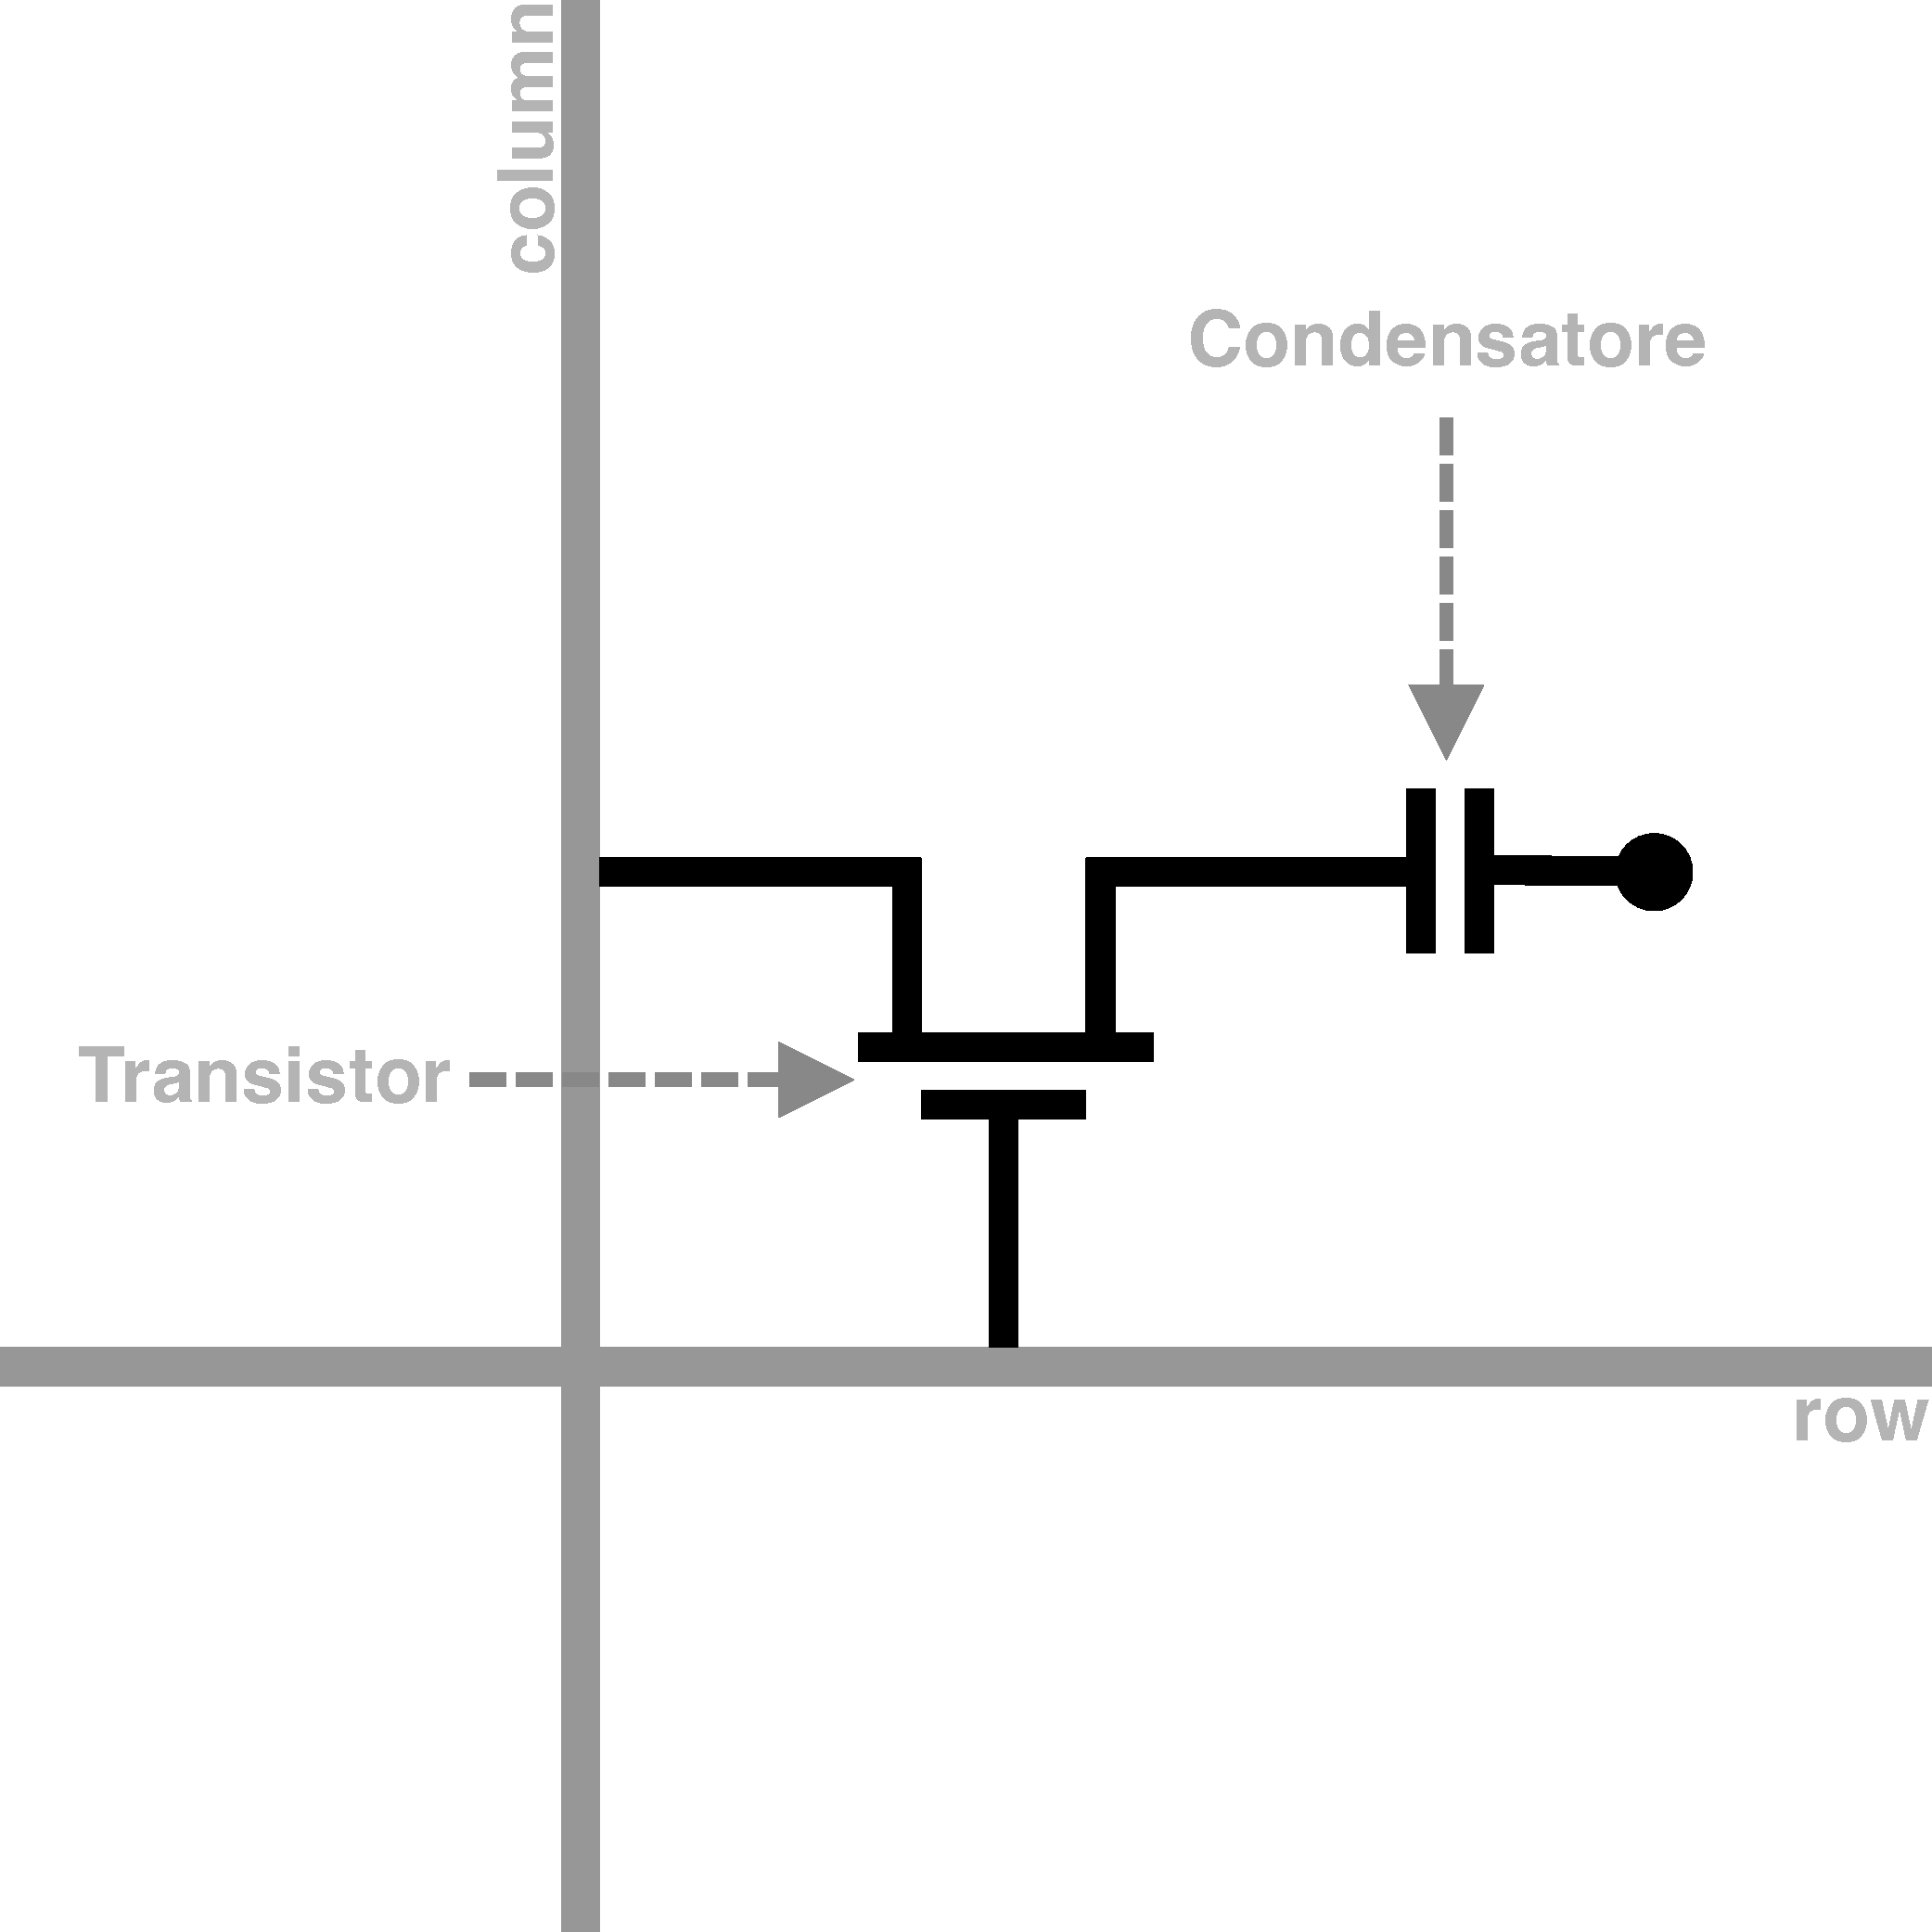
\includegraphics[width=0.6\linewidth]{images/5_memory/dram_bit_details.pdf}
		%\caption{PROM: nota la finestrella posta nella parte superiore del  circuito, che permette di ricevere i raggi UV}
	\end{figure}
	
\end{frame}


\begin{frame}
	\frametitle{La DRAM: dynamic RAM}
	 
	\begin{figure}[!htbp] 
		\centering
		%\advance\leftskip-0.25cm
		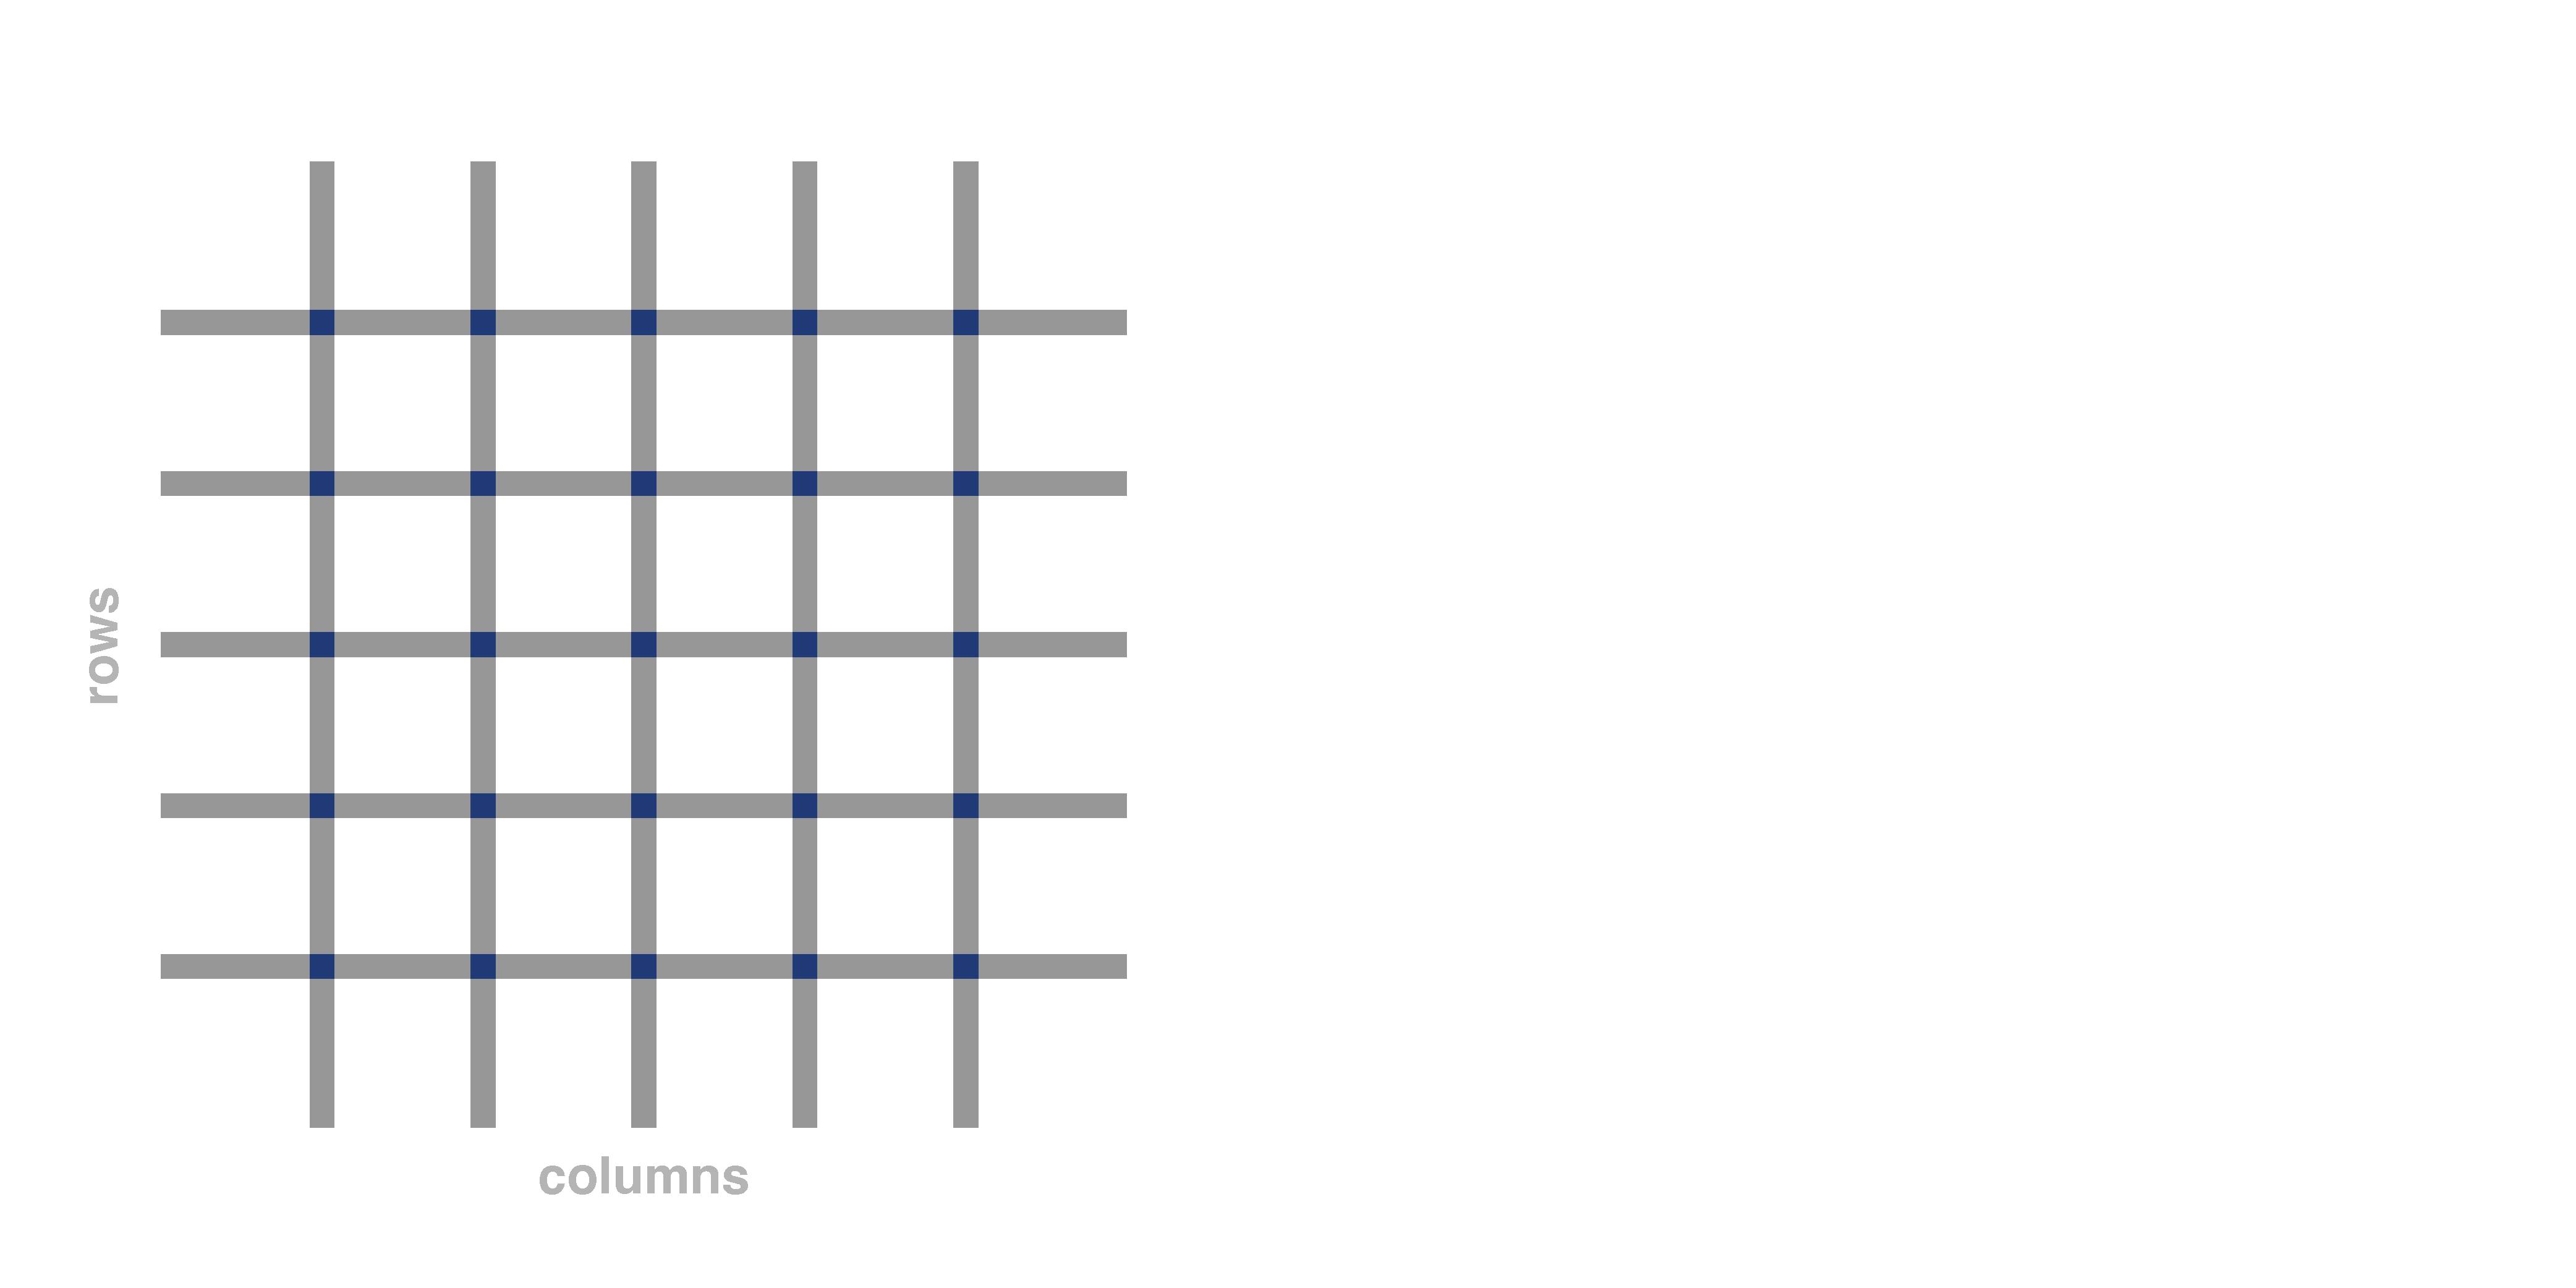
\includegraphics[width=1.0\linewidth]{images/5_memory/dram_matrix_1.pdf}
		%\caption{PROM: nota la finestrella posta nella parte superiore del  circuito, che permette di ricevere i raggi UV}
	\end{figure}
	
\end{frame}

\begin{frame}
	\frametitle{La DRAM: dynamic RAM}
	 
	\begin{figure}[!htbp] 
		\centering
		%\advance\leftskip-0.25cm
		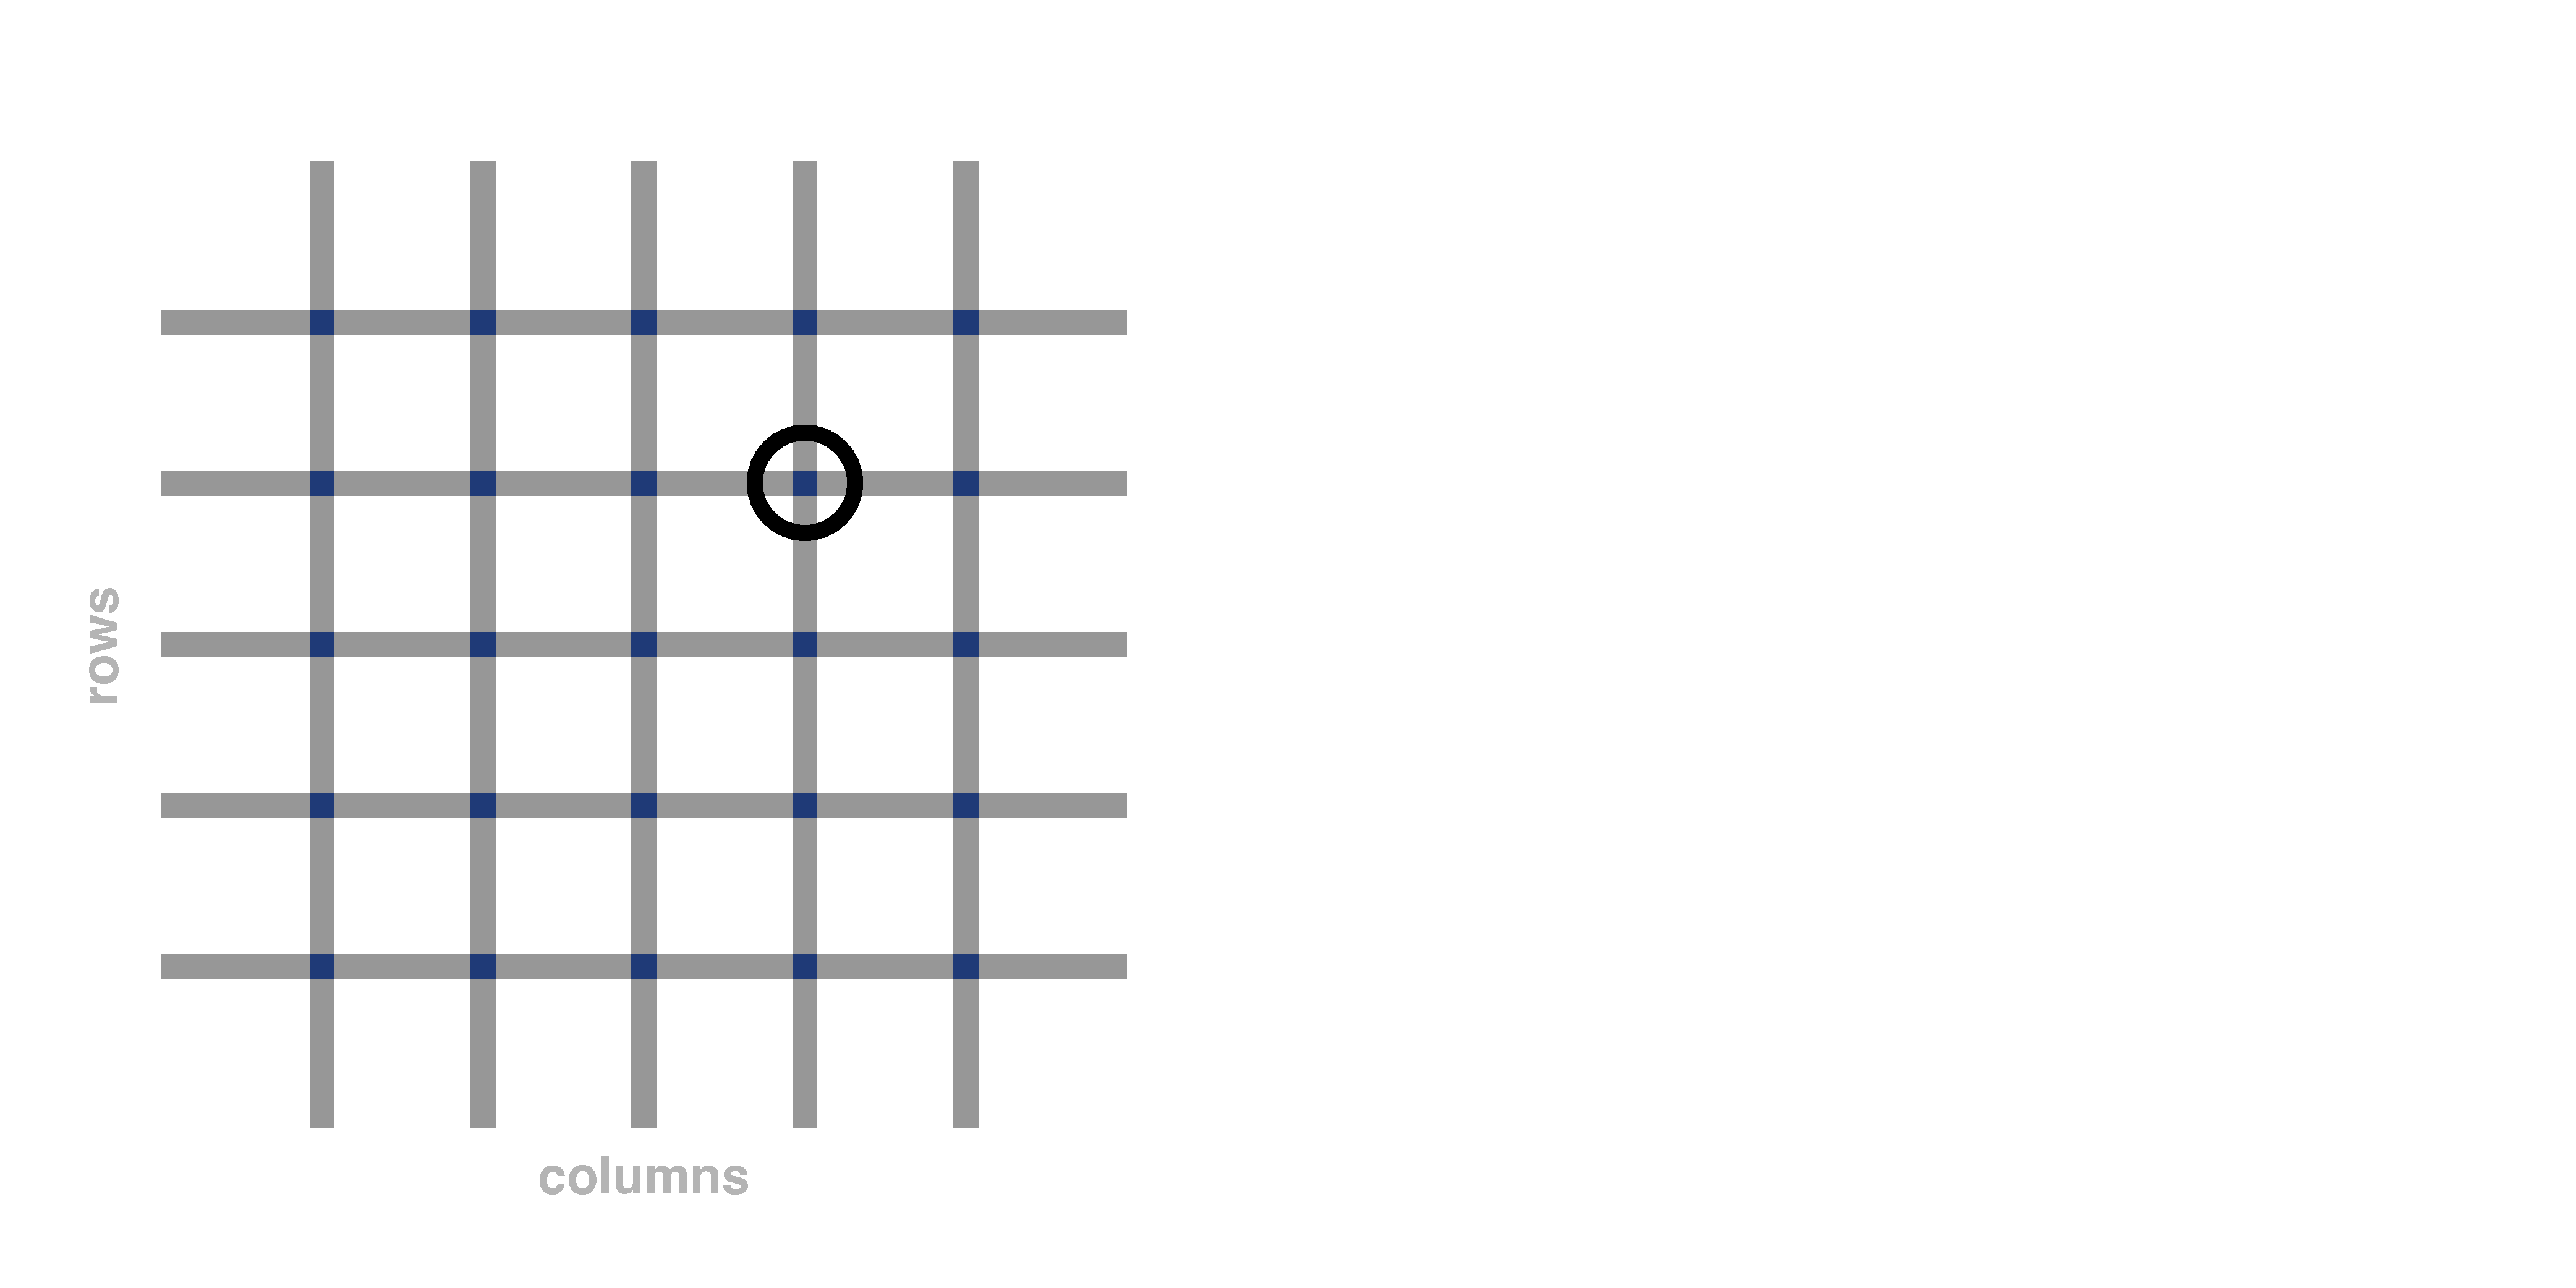
\includegraphics[width=1.0\linewidth]{images/5_memory/dram_matrix_2.pdf}
		%\caption{PROM: nota la finestrella posta nella parte superiore del  circuito, che permette di ricevere i raggi UV}
	\end{figure}
	
\end{frame}

\begin{frame}
	\frametitle{La DRAM: dynamic RAM}
	 
	\begin{figure}[!htbp] 
		\centering
		%\advance\leftskip-0.25cm
		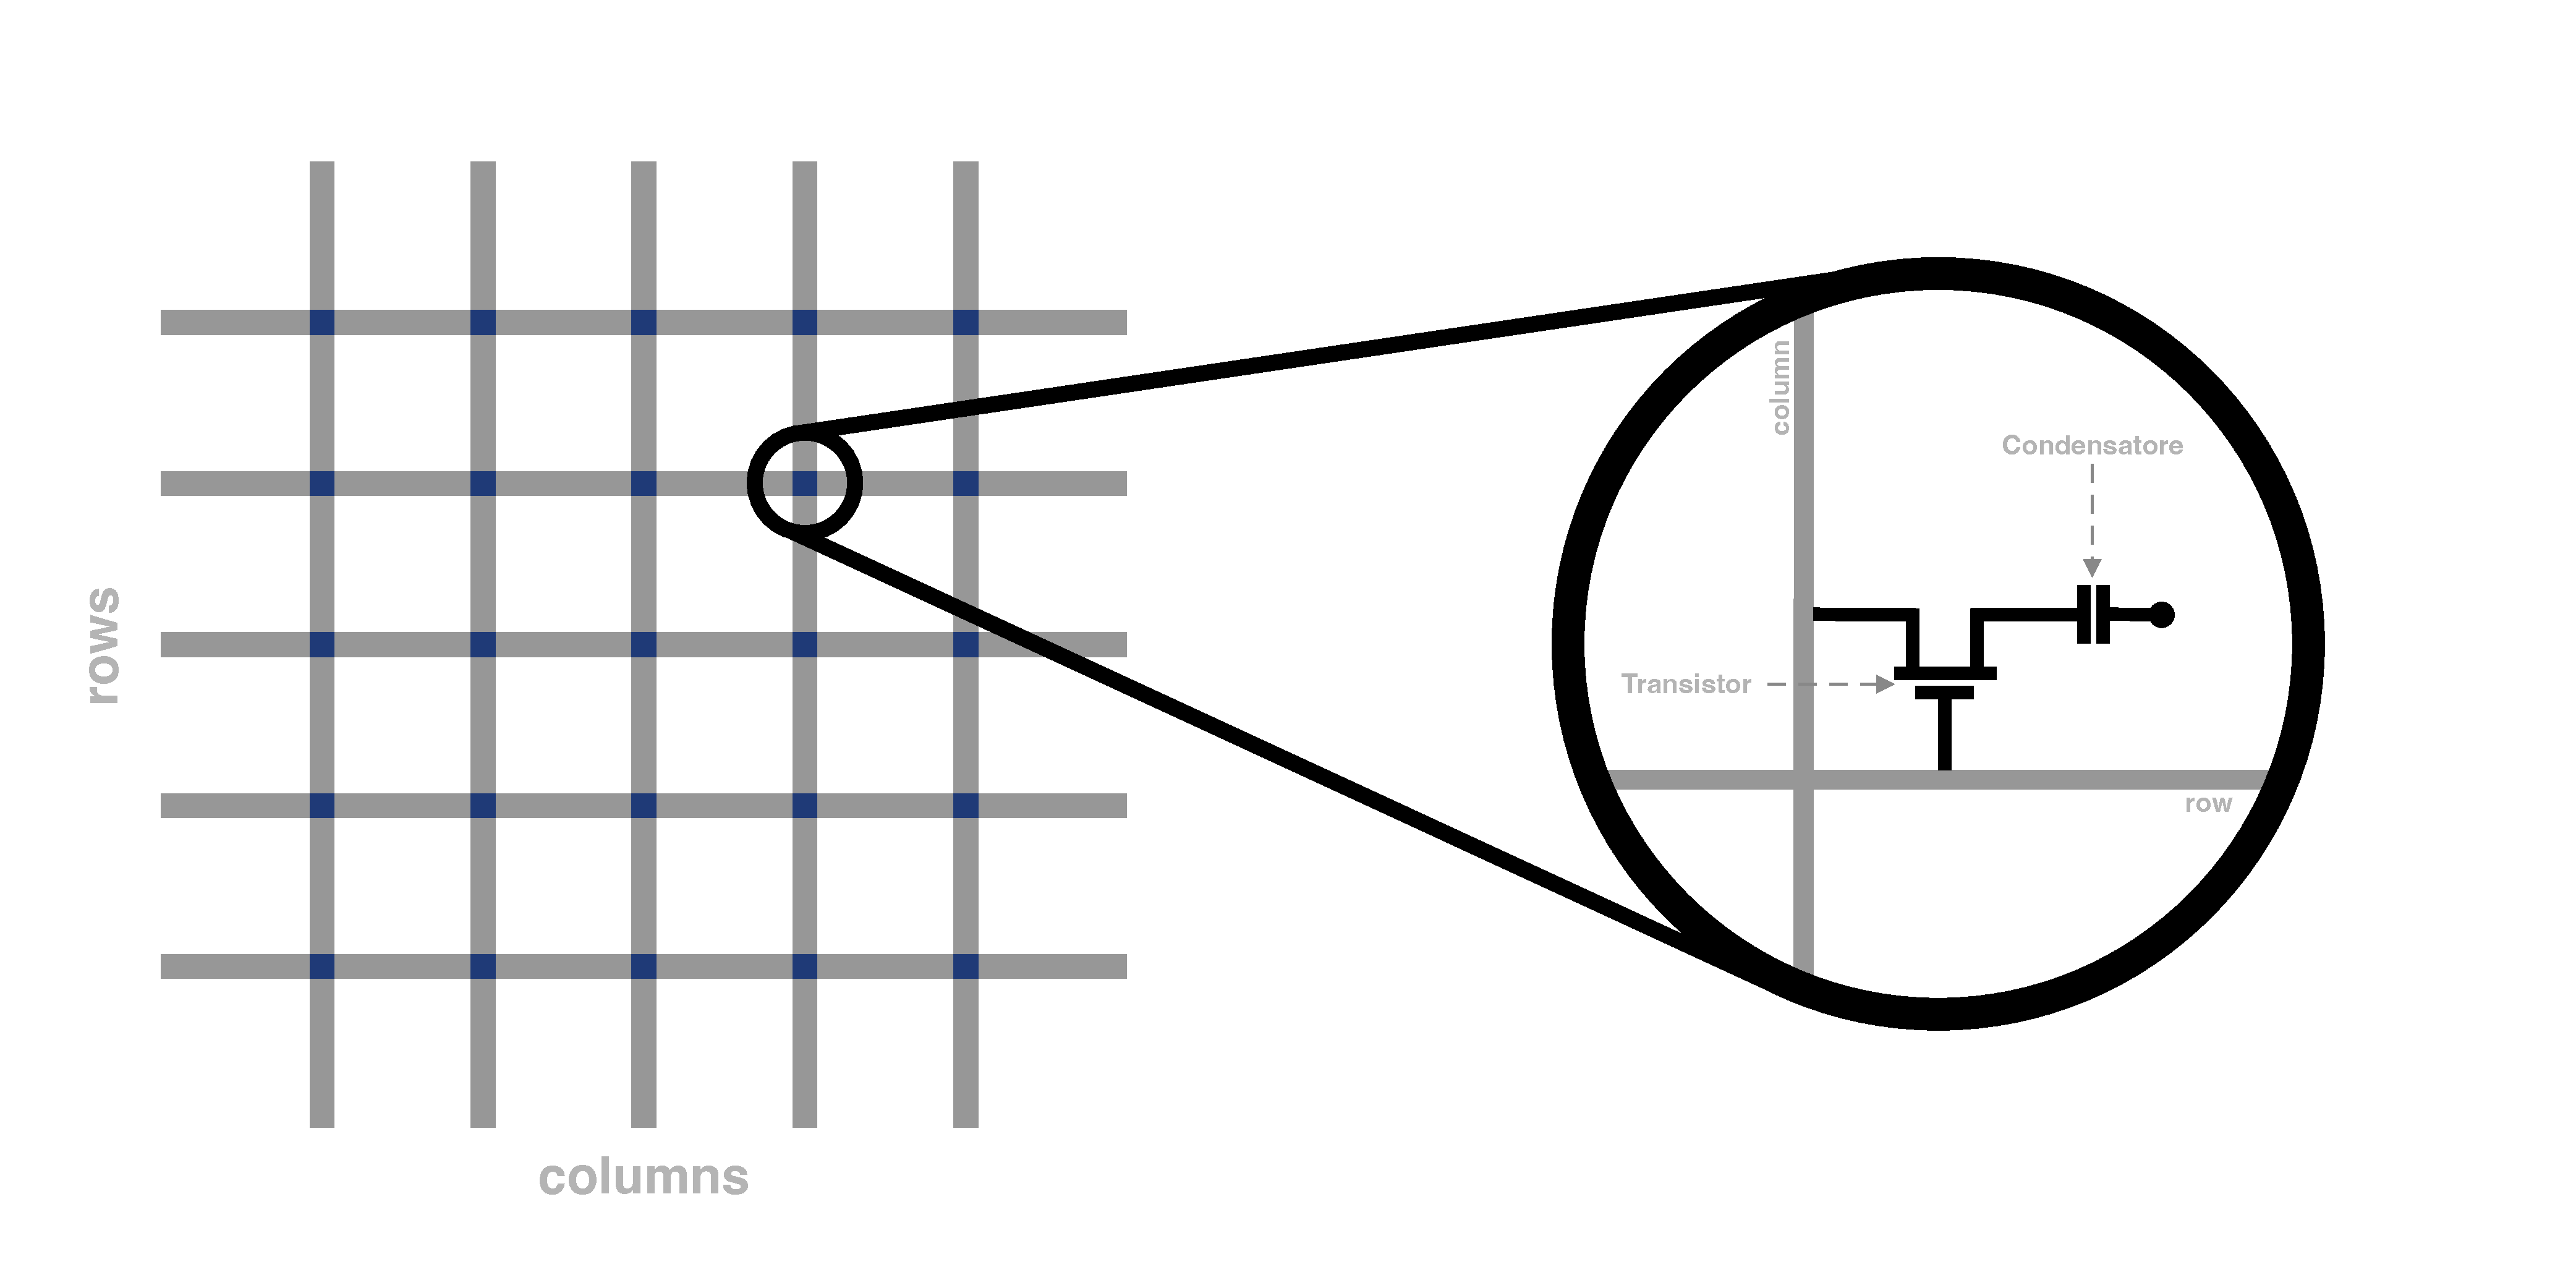
\includegraphics[width=1.0\linewidth]{images/5_memory/dram_matrix_3.pdf}
		%\caption{PROM: nota la finestrella posta nella parte superiore del  circuito, che permette di ricevere i raggi UV}
	\end{figure}
	
\end{frame}


\begin{frame}
	\frametitle{La DRAM: dynamic RAM}
	 
%	\begin{block}{Le prestazioni della memoria RAM}
%		Una delle strategie adottate per migliorare le prestazioni consiste nel combinare tipi di memoria veloce con tipi di memoria più capienti ma lente: un sistema gerarchico di memorie.
%	\end{block}
	
	\begin{figure}[!htbp] 
		\centering
		%\advance\leftskip-0.25cm
		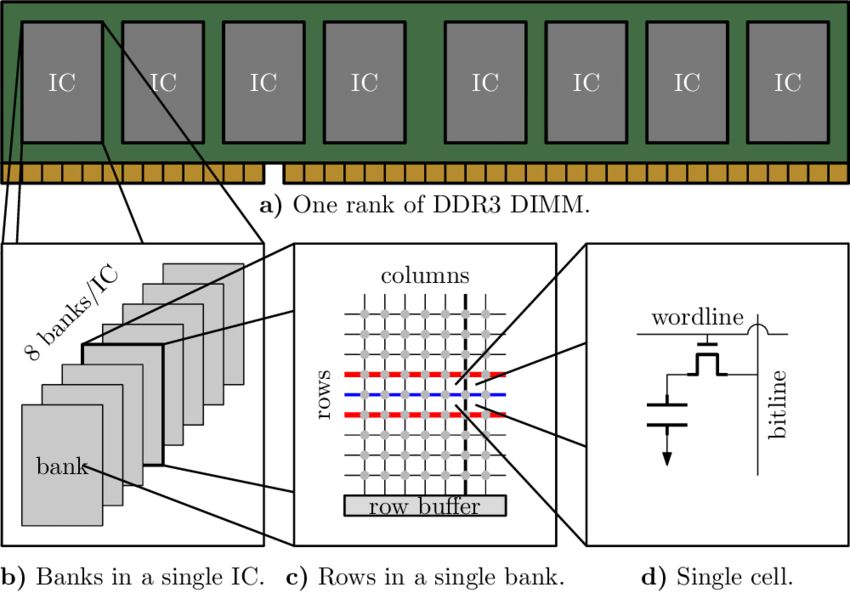
\includegraphics[width=0.8\linewidth]{images/5_memory/dram_organization.png}
%		\caption{La CPU: CU, ALU e registri}
		\label{fig:memory_dram_organization}
	\end{figure} 

\end{frame}


\begin{frame}
	\frametitle{La DRAM: dynamic RAM}
	
	\begin{columns}			
		\column{0.45\linewidth}
		\begin{scriptsize}
			\begin{figure}[!htbp]
				\centering
				\vspace{0.5em}
				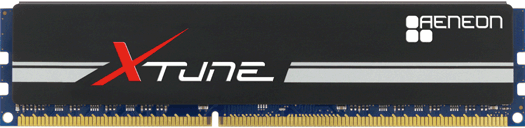
\includegraphics[width=0.9\linewidth]{images/5_memory/ddr3.png}
				\\DDR3 SDRAM - 240 pin - 5,25x1,18 inch\\\vspace{0.9em}
				
				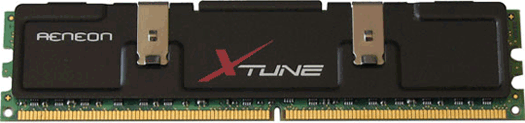
\includegraphics[width=0.9\linewidth]{images/5_memory/ddr2.png}
				\\DDR2 SDRAM - 240 pin - 5,25x1,18 inch\\\vspace{0.5em}
				
				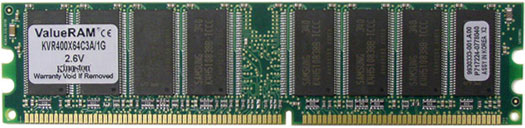
\includegraphics[width=0.9\linewidth]{images/5_memory/ddr1.png}
				\\DDR SDRAM - 184 pin - 5,375x1 inch\\\vspace{1em}
			\end{figure}
		\end{scriptsize}

		
		
		\column{0.55\linewidth}
		\begin{figure}[!htbp]
			\centering 
			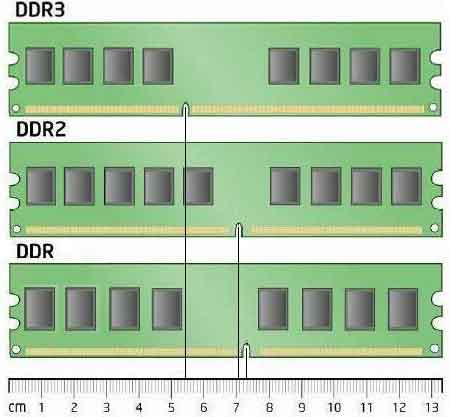
\includegraphics[width=1.0\linewidth]{images/5_memory/ddr_compare.png}
%			\caption{Confronto tra le diverse tipologie di DDR} 
		\end{figure}
	\end{columns}

\end{frame}


\begin{frame}
	\frametitle{La DRAM: dynamic RAM}
	 
	\begin{figure}[!htbp] 
		\centering
		%\advance\leftskip-0.25cm
		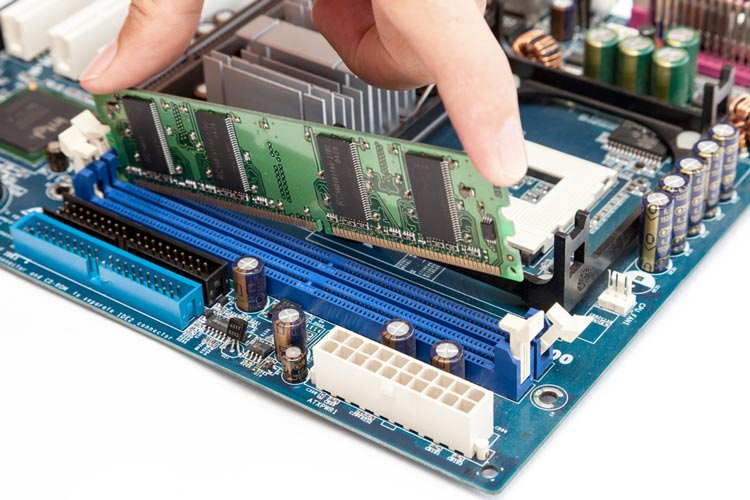
\includegraphics[width=0.9\linewidth]{images/5_memory/ram_installation.jpg}
		%\caption{}
	\end{figure}
	
\end{frame}


\begin{frame}
	\frametitle{La DRAM: dynamic RAM}
	 
%	La memoria RAM per PC viene realizzata in moduli:

	\begin{columns}			
		\column{0.5\linewidth}
		\begin{figure}[!htbp]
			\centering 
			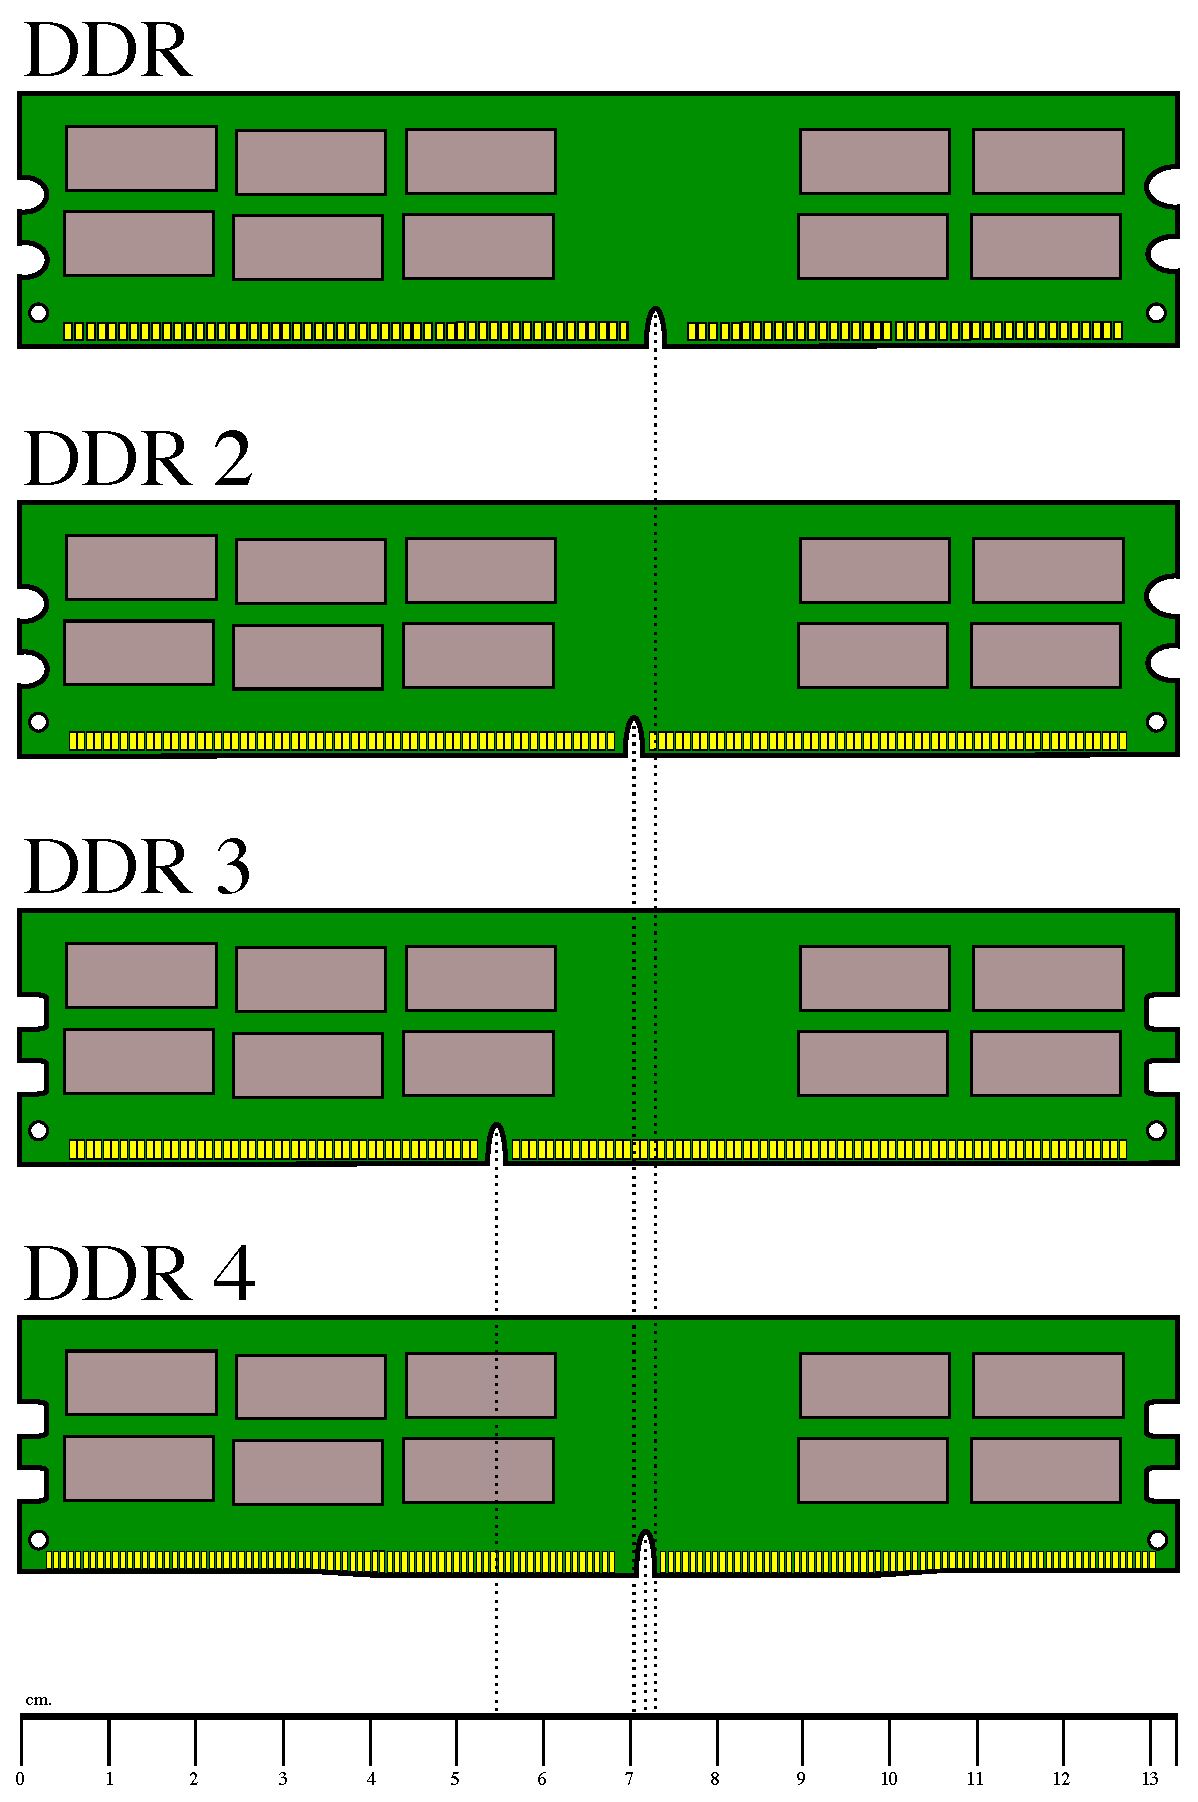
\includegraphics[width=0.63\linewidth]{images/5_memory/dimm.pdf}
			\caption{Per PC desktop: \protect\linebreak DIMM (Dual Inline Memory Module)}
			\label{fig:memory_dimm}
		\end{figure}

		\column{0.5\linewidth}
		\begin{figure}[!htbp]
			\centering 
			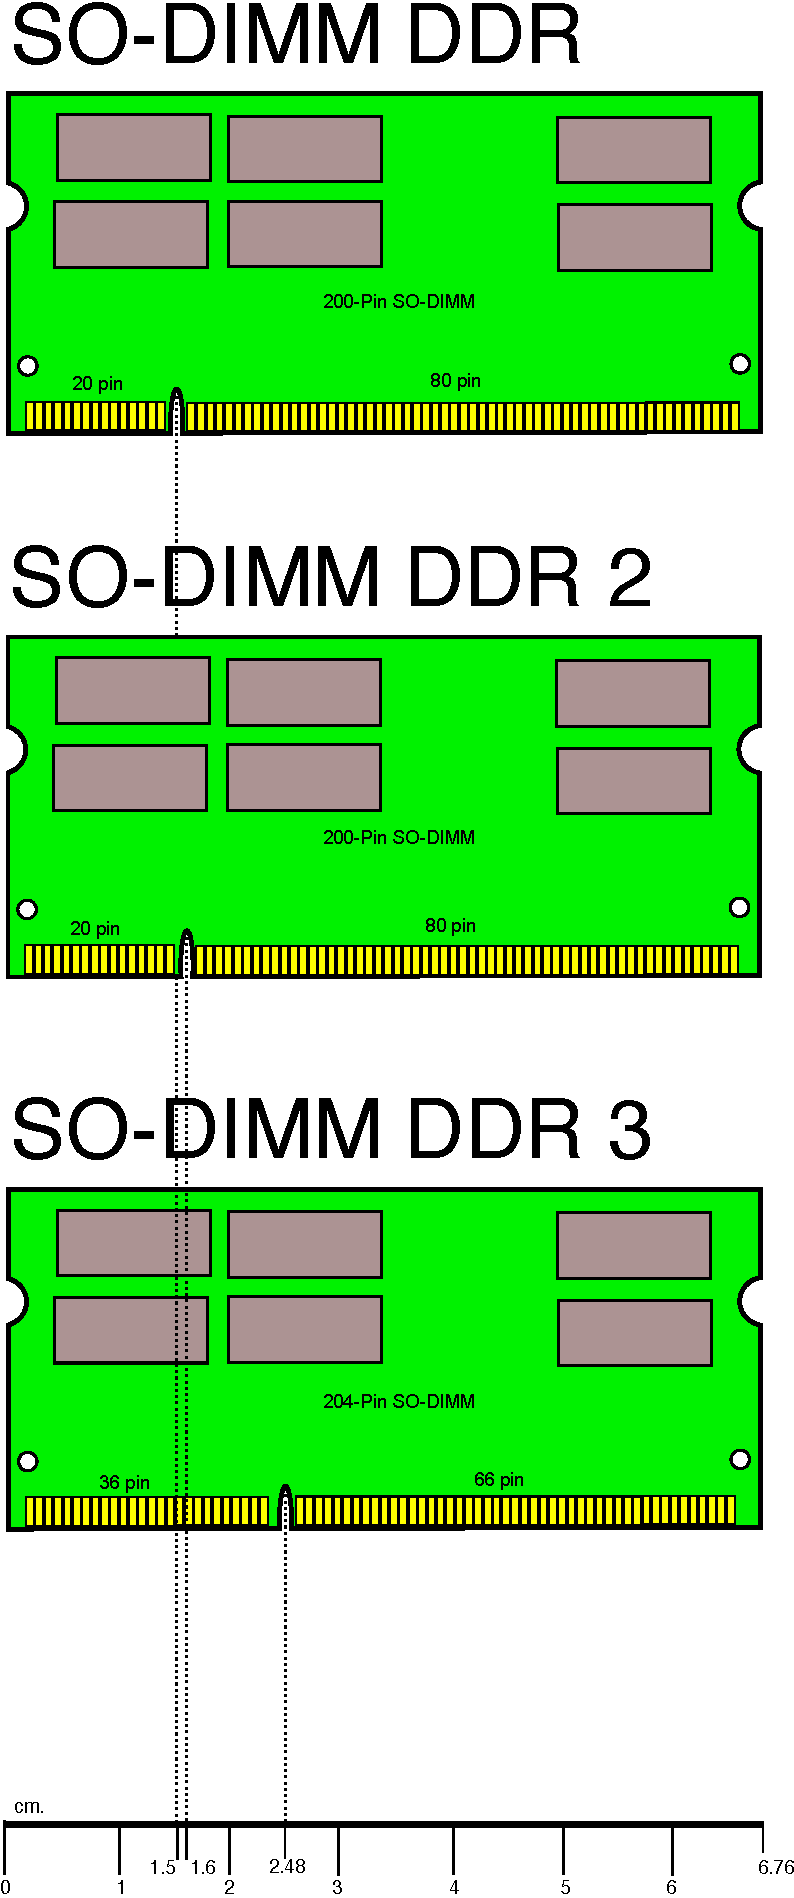
\includegraphics[width=0.4\linewidth]{images/5_memory/so_dimm.pdf}
			\caption{Per PC notebook: \protect\linebreak SO-DIMM (Small Outline DIMM)}
			\label{fig:memory_so_dimm}
		\end{figure}
	\end{columns}
	
\end{frame}




\begin{frame}
	\frametitle{La DRAM: dynamic RAM}
	 
	\begin{figure}[!htbp] 
		\centering
		%\advance\leftskip-0.25cm
		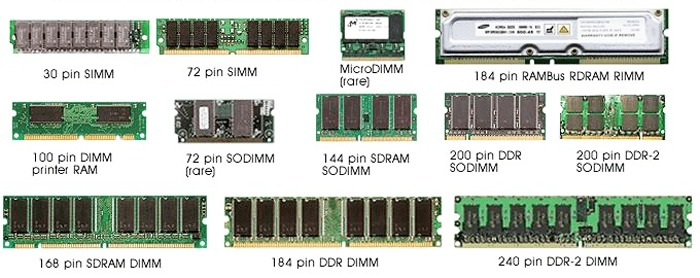
\includegraphics[width=1.0\linewidth]{images/5_memory/ram_types.jpeg}
		%\caption{}
	\end{figure}
	
\end{frame}






%\subsubsection[La SDRAM: synchronized dynamic RAM]{La SDRAM: synchronized dynamic RAM}
% https://www.nexthardware.com/forum/ram/41922-latenze-ram-parametri-e-descrizione-cura-di-swarzy.html
\begin{frame}
	\frametitle{La RAM: valutare le prestazioni di una RAM}
	
	\begin{block}{}
		La velocità di trasferimento è notevolmente influenzata dai fenomeni di latenza, che si verificano durante le operazioni di lettura/scrittura e che dipendono strettamente dal tipo e dalla qualità del chip, nonché dalla frequenza di funzionamento. Ad ogni banco di memoria vengono associati dei tempi caratteristici detti timing, misurati in unità di cicli di clock: a valori più bassi corrispondono prestazioni migliori, a parità di frequenza.\\~\\
		
		I timing più importanti sono (vedi \underline{\href{https://it.wikipedia.org/wiki/DDR\_SDRAM}{link}}):
		\begin{itemize}
			\item CAS Latency Time (tCl)
			\item RAS to CAS Delay Time (tRCD)
			\item RAS Precharge Time (tRP)
			\item Active-to-Precharge Delay (tRAS)
			\item Row Cycle Time (tRC)
		\end{itemize}
		
	\end{block}
	
\end{frame}



\subsubsection[La SRAM: static RAM]{La SRAM: static RAM}
\begin{frame}
	\frametitle{La SRAM: static RAM}
	  
	\begin{block}{}
		Le \textbf{SRAM}, acronimo di static RAM, sono sempre memorie volatili ma non necessitano di refresh. I flip-flop sono alla base della memorizzazione di un singolo bit in queste tipologie di memoria.\\~\\
		I banchi di SRAM consentono di mantenere le informazioni per un tempo teoricamente infinito, hanno \textbf{bassi tempi di lettura} e \textbf{bassi consumi}. La necessità di usare molti componenti per cella le rende però \textbf{più costose} delle DRAM.\\~\\
		Sono solitamente usate per le memorie cache, dove elevate velocità e ridotti consumi sono caratteristiche fondamentali. Ad esempio, possono essere trovate nella cache L1, L2 o L3 di un processore.
		
	\end{block}
\end{frame}


% https://superuser.com/questions/196143/where-exactly-l1-l2-and-l3-caches-located-in-computer
\begin{frame}
	\frametitle{La DRAM: dynamic RAM}
	 
	\begin{figure}[!htbp] 
		\centering
		%\advance\leftskip-0.25cm
		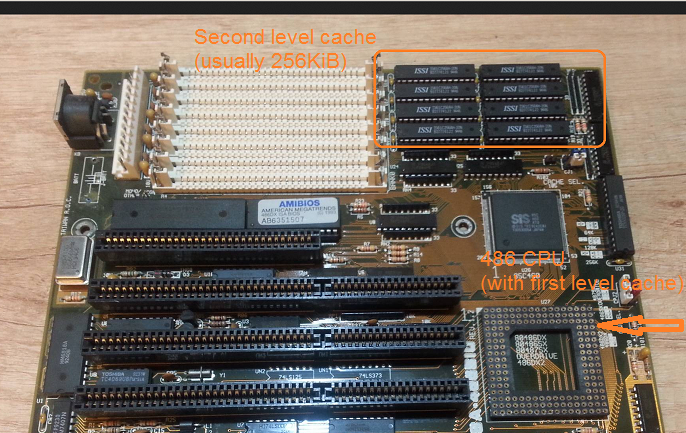
\includegraphics[width=0.62\linewidth]{images/5_memory/cache_1.png}
		\caption{\textbf{80486 (1989):} questa è la prima CPU di questa generazione che ha un po' di cache sulla CPU. È una cache unificata da 8 KB, il che significa che viene utilizzata per dati e istruzioni. In questo periodo diventa comune inserire 256 KB di memoria statica veloce sulla scheda madre come cache di 2° livello. Quindi cache di 1° livello sulla CPU, cache di 2° livello sulla scheda madre.}
	\end{figure}
	
\end{frame}


\begin{frame}
	\frametitle{La DRAM: dynamic RAM}
	 
	\begin{figure}[!htbp] 
		\centering
		%\advance\leftskip-0.25cm
		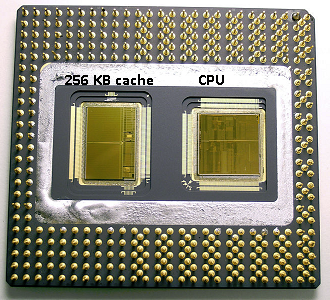
\includegraphics[width=0.42\linewidth]{images/5_memory/cache_2.png}
		\caption{\textbf{\href{https://en.wikipedia.org/wiki/Pentium\_Pro}{Pentium Pro '80686'} (1995):} a seconda del modello, questo chip aveva una cache integrata da 256Kb, 512KB o 1MB. Si noti che metà dello spazio nel chip è utilizzato dalla cache. E questo è per il modello da 256KB. Il prezzo di mercato era piuttosto alto per l'epoca. Si noti inoltre che questo chip contiene due matrici. Uno con la CPU e la prima cache, l'altro con la seconda cache da 256 KB.}
	\end{figure}
	
\end{frame}


\begin{frame}
	\frametitle{La DRAM: dynamic RAM}
	 
	\begin{figure}[!htbp] 
		\centering
		%\advance\leftskip-0.25cm
		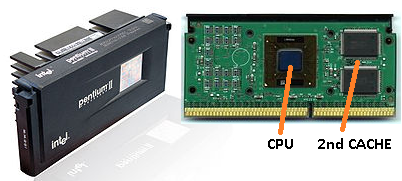
\includegraphics[width=0.8\linewidth]{images/5_memory/cache_3.png}
		\caption{\textbf{\href{https://en.wikipedia.org/wiki/Pentium\_Pro}{Pentium-2}:} per ragioni economiche la seconda cache viene spostata fuori dalla CPU. Solo successivamente, man mano che la tecnologia è avanzata, diventò più accessibile dal punto di vista dei costi rimettere la seconda cache all'interno della CPU.}
	\end{figure}
	
\end{frame}



\begin{frame}
	\frametitle{La DRAM: dynamic RAM}
	 
	\begin{figure}[!htbp] 
		\centering
		%\advance\leftskip-0.25cm
		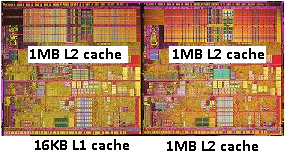
\includegraphics[width=0.8\linewidth]{images/5_memory/cache_4.png}
		\caption{\textbf{Pentium-D (duo):} che fondamentalmente corrispondono a due core pentium-4 sullo stesso chip. La cache di secondo livello viene condivisa tra i due core, una cache di secondo livello condivisa è globalmente più veloce di avere due cache di secondo livello indipendenti di dimensioni dimezzate.}
	\end{figure}
	
\end{frame}


\begin{frame}
	\frametitle{La DRAM: dynamic RAM}
	 
	\begin{figure}[!htbp] 
		\centering
		%\advance\leftskip-0.25cm
		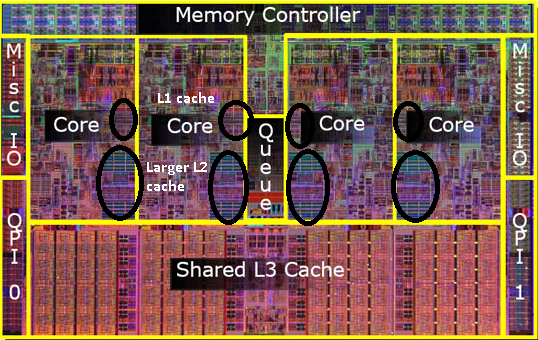
\includegraphics[width=0.8\linewidth]{images/5_memory/cache_5.png}
		\caption{\textbf{Processore i7:} più cores, stesso ragionamento, usando una cache di terzo livello condivisa tra i core.}
	\end{figure}

\end{frame}


\subsubsection[Le prestazioni delle memorie]{Le prestazioni delle memorie}
\begin{frame}
	\frametitle{Le prestazioni delle memorie}
	
	\begin{block}{}
		Per valutare le prestazioni di una memoria utilizziamo:
		\begin{itemize}
			\item \textbf{latency}: la latenza della memoria è il tempo (la latenza) che intercorre tra l'avvio di una richiesta per un byte o una parola in memoria e il momento in cui viene recuperato dal processore.\\
				Se i dati non sono nella cache del processore, ci vorrà più tempo per ottenerli, poiché il processore dovrà comunicare con le celle di memoria esterne. La latenza è quindi una misura fondamentale della velocità della memoria: minore è la latenza, più veloce è l'operazione di lettura.
				La latenza può essere espressa in cicli di clock o in tempo misurato in nanosecondi. \pause
			\item \textbf{bandwidth}: la larghezza di banda della memoria misura il throughput della memoria, ovvero la quantità di informazioni al secondo che viene trasmessa dalla memoria.
		\end{itemize}
		
	\end{block}
	
\end{frame}


\subsection[L'indirizzamento di memoria]{L'indirizzamento di memoria}
\begin{frame}
	\frametitle{L'indirizzamento di memoria}
	  
	\begin{block}{}
	
		Il modello usuale di una memoria principale è lineare; in tale modello la memoria è costituita di parole o celle numerate da 0 fino al valore massimo. Il numero che identifica ogni cella è detto \textbf{indirizzo}.\\~\\ \pause
	
		La dimensione di ogni cella indirizzabile dipende dal tipo di calcolatore, comunque è multiplo di un byte.\\~\\ \pause
		
		È opportuno distinguere la \textbf{dimensione} (effettiva) di una memoria dal suo \textbf{spazio di indirizzamento}: lo spazio di indirizzamento è il numero massimo di indirizzi possibili della memoria e dipende dalla lunghezza dell'indirizzo, cioè dal numero di bit che costituiscono l'indirizzo (o equivalentemente la dimensione del BUS degli indirizzi); se $N$ è il numero di bit che costituiscono l'indirizzo di una memoria allora il suo spazio di indirizzamento è $2^N$ (due elevato alla $N$).
		
	\end{block}
\end{frame}



\subsubsection[Lo spazio di indirizzamento]{Lo spazio di indirizzamento}
\begin{frame}
	\frametitle{L'indirizzamento di memoria}
	  
	\begin{block}{Lo spazio di indirizzamento}
	
		\begin{columns}			
			\column{0.52\linewidth}
			L’\textbf{indirizzo di memoria} di ciascuna cella è definito dalla posizione relativa della cella rispetto alla prima cella.\\~\\
			Riassumendo se $N$ è l'ampiezza del BUS degli indirizzi, ovvero il numero di fili conduttori sul BUS degli indirizzi:
			\begin{itemize}
				\item \textbf{spazio di indirizzamento} = $2^N$
				\item \textbf{indirizzo ultima cella} = $2^N - 1$ (corrisponde a $n$ uni in binario, nell'esempio a destra $N=3$)
			\end{itemize}
			
	
			\column{0.48\linewidth}
			\begin{figure}[!htbp]
				\centering 
				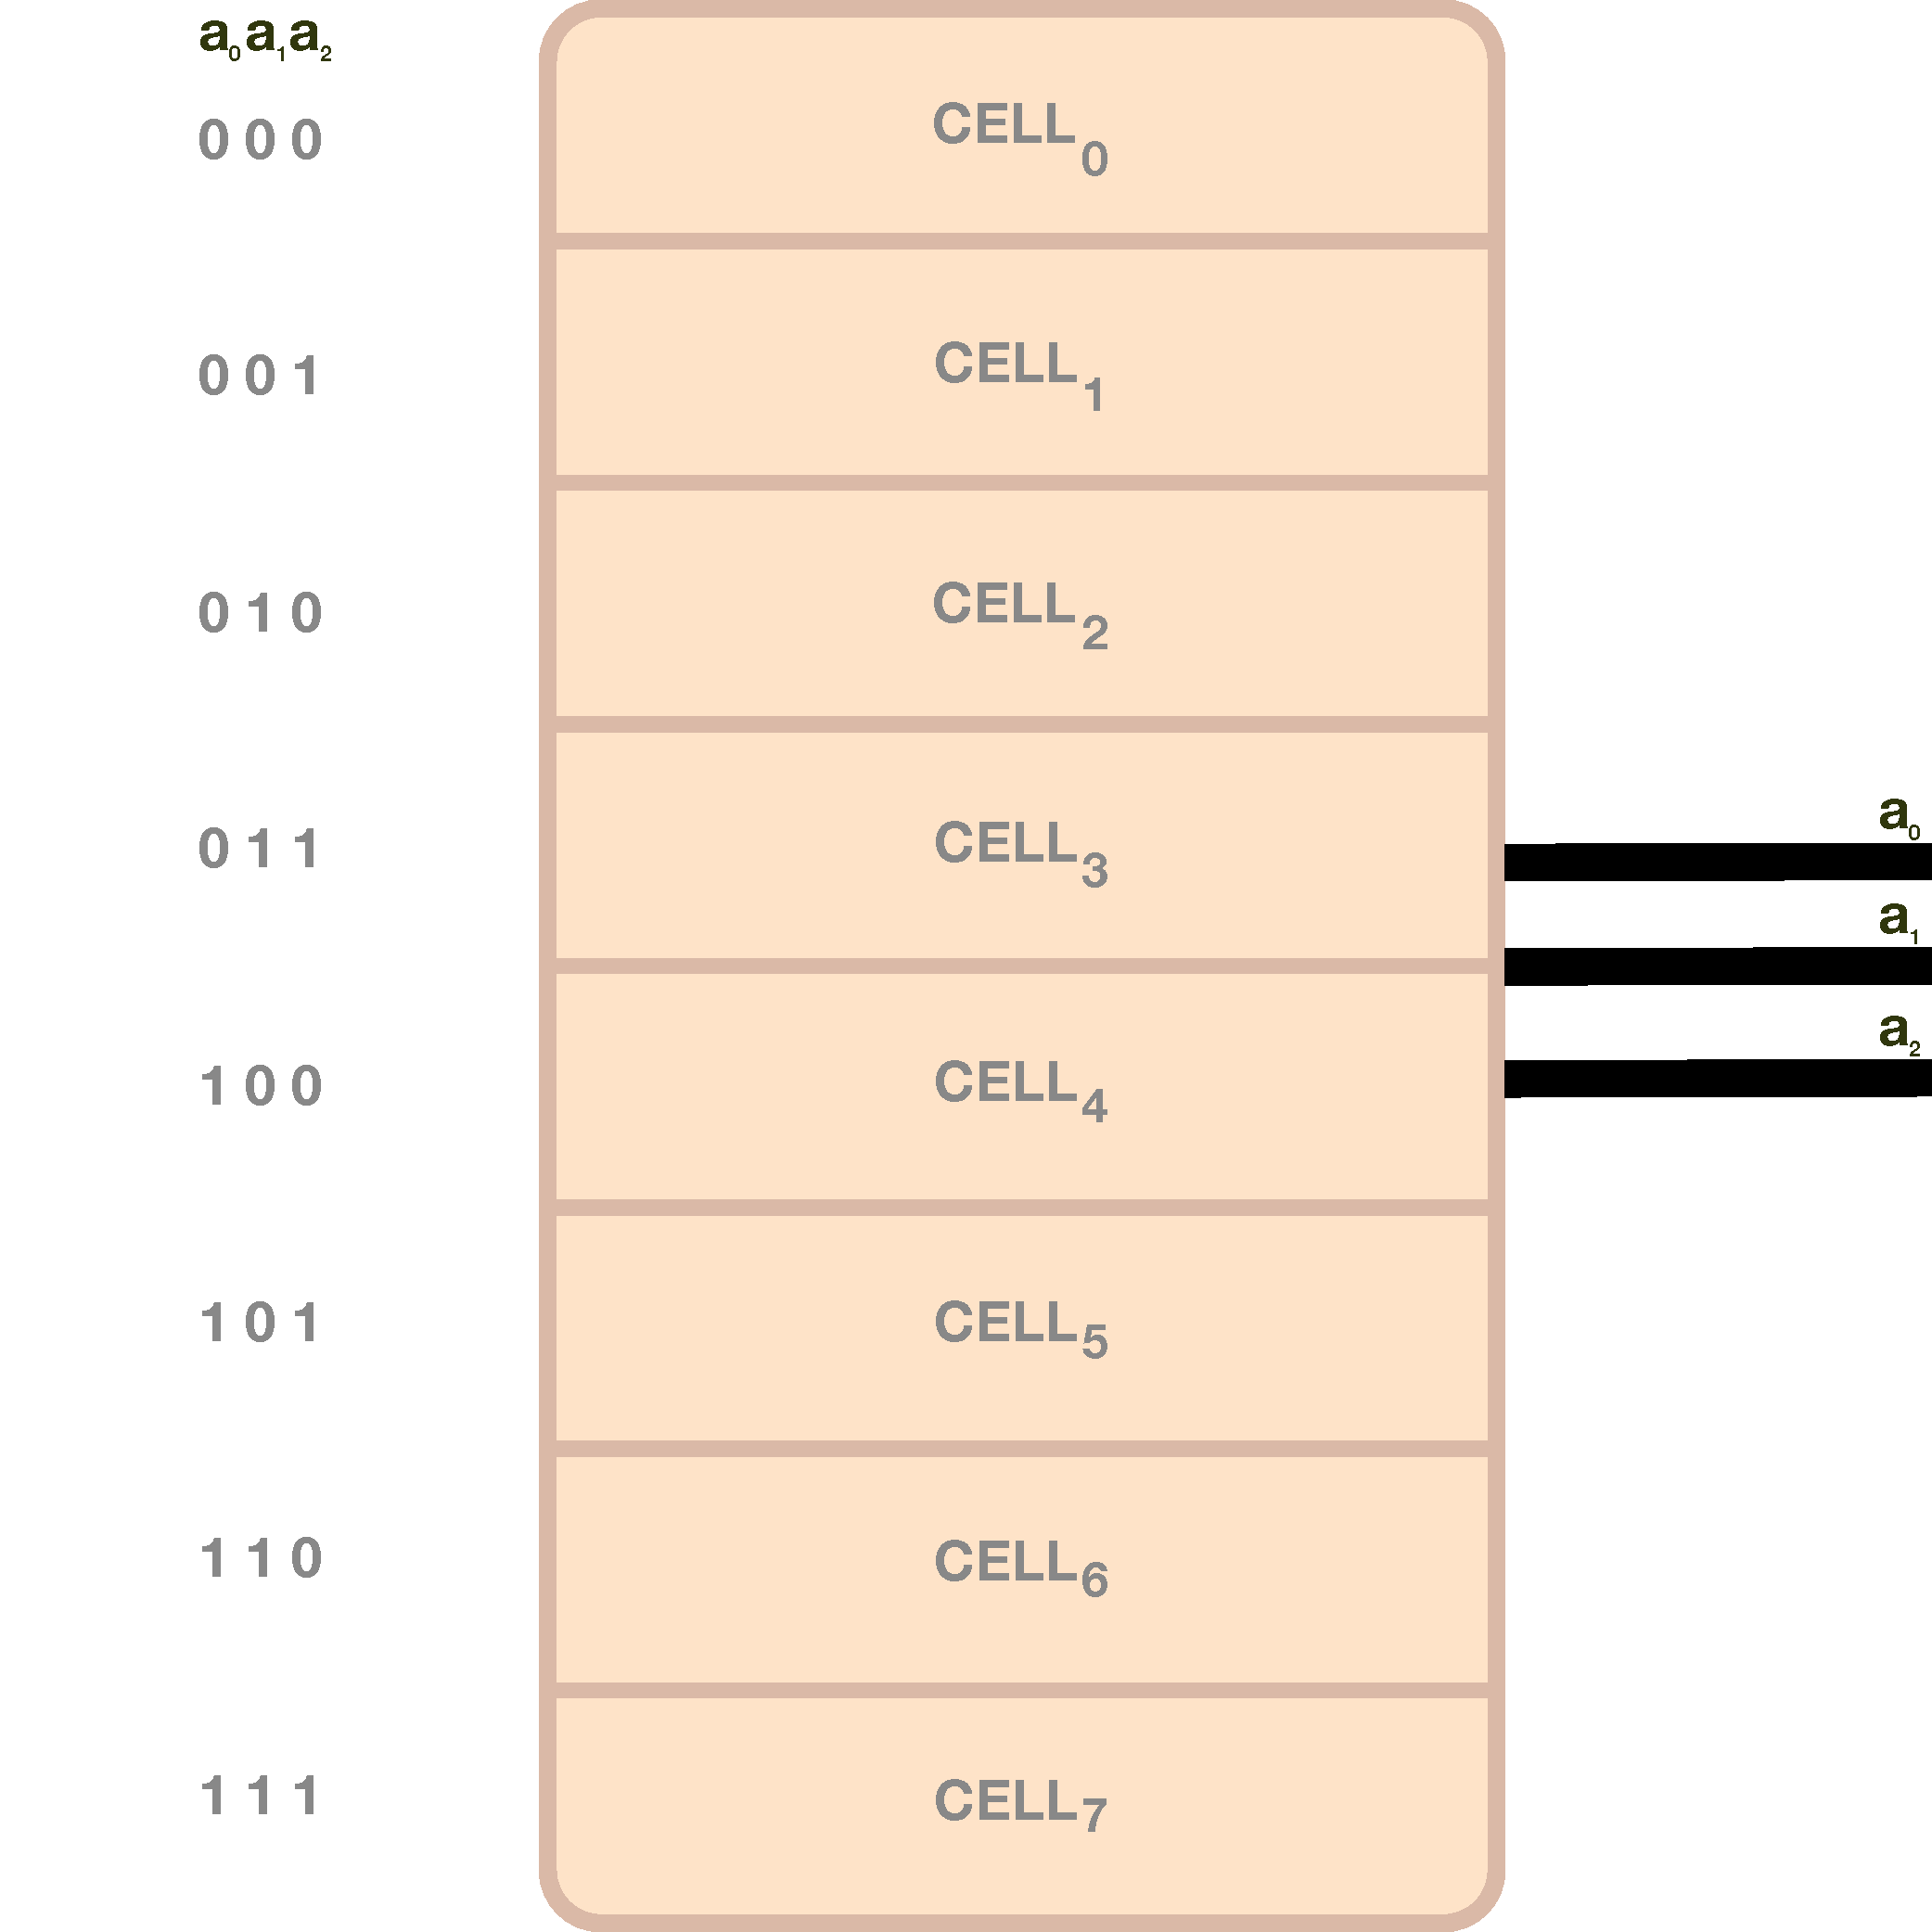
\includegraphics[width=1.0\linewidth]{images/5_memory/memory_address.pdf}
				%\caption{Esempio di memoria indirizzata tramite un BUS degli indirizzi di ampiezza 3 bit}
			\end{figure}
		\end{columns}
		
	\end{block}
\end{frame}


\begin{frame}
	\frametitle{L'indirizzamento di memoria}
	
	\begin{figure}[!htbp]
		\centering 
		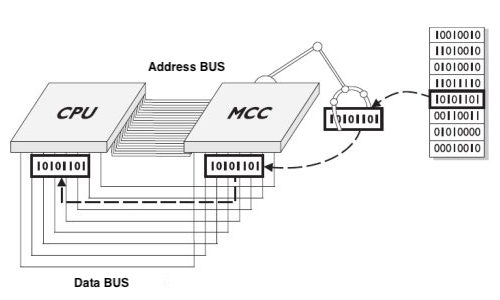
\includegraphics[width=0.85\linewidth]{images/5_memory/mcc.png}
		\caption{Il Memory Controller Chip (MCC) può prendere qualunque byte della RAM per porlo sul data BUS affinché la CPU possa leggerlo}
%			\label{fig:memory_so_dimm}
	\end{figure}
\end{frame}






% \scalebox{0.90}{}
\subsubsection[Multipli del byte]{Multipli del byte}
\begin{frame}
	\frametitle{L'indirizzamento di memoria}
	
	\begin{block}{Multipli del byte}
		\begin{table}[]
			\centering
			\begin{tabular}{llclcl}
			%\hline
			$1kB$ & kilobyte & = & 1024 B & = & $2^{10}B$ \\
			$1MB$ & megabyte & = & 1024 kB & = & $1024^2$ B \\
			$1GB$ & gigabyte & = & 1024 MB & = & $1024^2$ kB \\
			$1TB$ & terabyte & = & 1024 GB & = & $1024^2$ kB \\
			$1PB$ & petabyte & = & 1024 TB & = & $1024^3$ kB \\
			$1EB$ & exabyte & = & 1024 PB & = & $1024^4$ kB \\
			%$1ZB$ & zettabyte & = & 1024 EB & = & $1024^5$ kB \\
			%$1YB$ & yottabyte & = & 1024 ZB & = & $1024^6$ kB \\
			\end{tabular}
		\end{table}		
	\end{block}
	
	\begin{block}{Ricorda inoltre che:}
		\begin{table}[]
			\centering
			\begin{tabular}{llclcl}
			%\hline
			$1k$ & $=$ & $2^{10}$ & $\simeq$ & $10^3$  \\
			$1M$ & $=$ & $2^{20}$ & $\simeq$ & $10^6$  \\
			$1G$ & $=$ & $2^{30}$ & $\simeq$ & $10^9$  \\
			\end{tabular}
		\end{table}		
	\end{block}
\end{frame}




\subsubsection[La dimensione di memoria indirizzabile]{La dimensione di memoria indirizzabile}
\begin{frame}
	\frametitle{L'indirizzamento di memoria}
	
	\begin{block}{Lo spazio di indirizzamento}
		\begin{table}[]
			\centering
			\begin{tabular}{lcl}
			%\hline
			$10bit$ & = & $1k$ celle (1024 celle) \\
			$16bit$ & = & $64k$ celle (65536 celle) \\
			$20bit$ & = & $1M$ celle (RAM dei processori fino all'80286) \\
%			$30bit$ & = & $1G$ celle  \\
			$32bit$ & = & $4G$ celle (RAM dei processori fino al Pentium) \\
			$36bit$ & = & $64G$ celle (RAM dei processori fino al Pentium IV)  \\
			$40bit$ & = & $1T$ celle (RAM dei processori fino all’Athlon 64)  \\
			$64bit$ & = & $16E$ celle (RAM dei processori fino al Core i7)  \\
			
			\end{tabular}
		\end{table}		
	\end{block}
	
	\begin{block}{La dimensione di memoria indirizzabile}
	
		Per conoscere la \textbf{dimensione di memoria indirizzabile} è necessario conoscere la \textbf{dimensione della cella}:\\
		
		\begin{scriptsize}
			Dimensione della memoria indirizzabile = spazio di indirizzamento $\cdot$ dimensione della cella
		\end{scriptsize}
		
	\end{block}
\end{frame}


\subsubsection[La dimensione effettiva di memoria]{La dimensione effettiva di memoria}
\begin{frame}
	\frametitle{L'indirizzamento di memoria}
	
	\begin{block}{La dimensione effettiva di memoria}
		La \textbf{dimensione della memoria} corrisponde al numero di byte che la costituiscono effettivamente.\\~\\
		Di conseguenza la \textbf{dimensione effettiva di memoria} è sempre minore o uguale alla \textbf{dimensione di memoria indirizzabile}.		
	\end{block}
	
	\begin{block}{Esempio: processori con indirizzi a 32 bit e 64 bit}
		Nei Personal Computer Intel in cui l'indirizzo è di 32 bit lo spazio di indirizzamento è di $2^{32}$ byte, infatti la memoria massima utilizzabile in tali sistemi è di 4 Giga byte.\\
		Attualmente la maggior parte dei processori usano indirizzi di 64 bit, la memoria effettiva in tal caso è sicuramente inferiore rispetto a quella indirizzabile ($32GB \ll 16EB$ ).
		
	\end{block}
\end{frame}

% TODO Aggiungere esercizi di calcolo delle memorie




\subsection[Le memorie permanenti]{Le memorie permanenti}
\begin{frame}
	\frametitle{Le memorie permanenti}
	  
	\begin{block}{Le memorie permanenti}
		Nel mondo dell'informatica, le unità di archiviazione svolgono un ruolo fondamentale nel conservare dati e programmi in modo permanente all'interno di un computer.\\~\\
		Tra le tecnologie più diffuse per l'\textbf{archiviazione permanente} ci sono:
		\begin{itemize}
			\item le \textbf{memorie flash}
			\item gli \textbf{Hard Disk Drive} (HDD)
			\item i \textbf{Solid State Drive} (SSD)
		\end{itemize}
		Queste unità differiscono significativamente nella loro struttura, prestazioni e caratteristiche, offrendo opzioni variegate per soddisfare le diverse esigenze degli utenti.
	\end{block}

\end{frame}

\begin{frame}
	\frametitle{Le memorie permanenti}
	
	\begin{figure}[!htbp]
		\centering 
		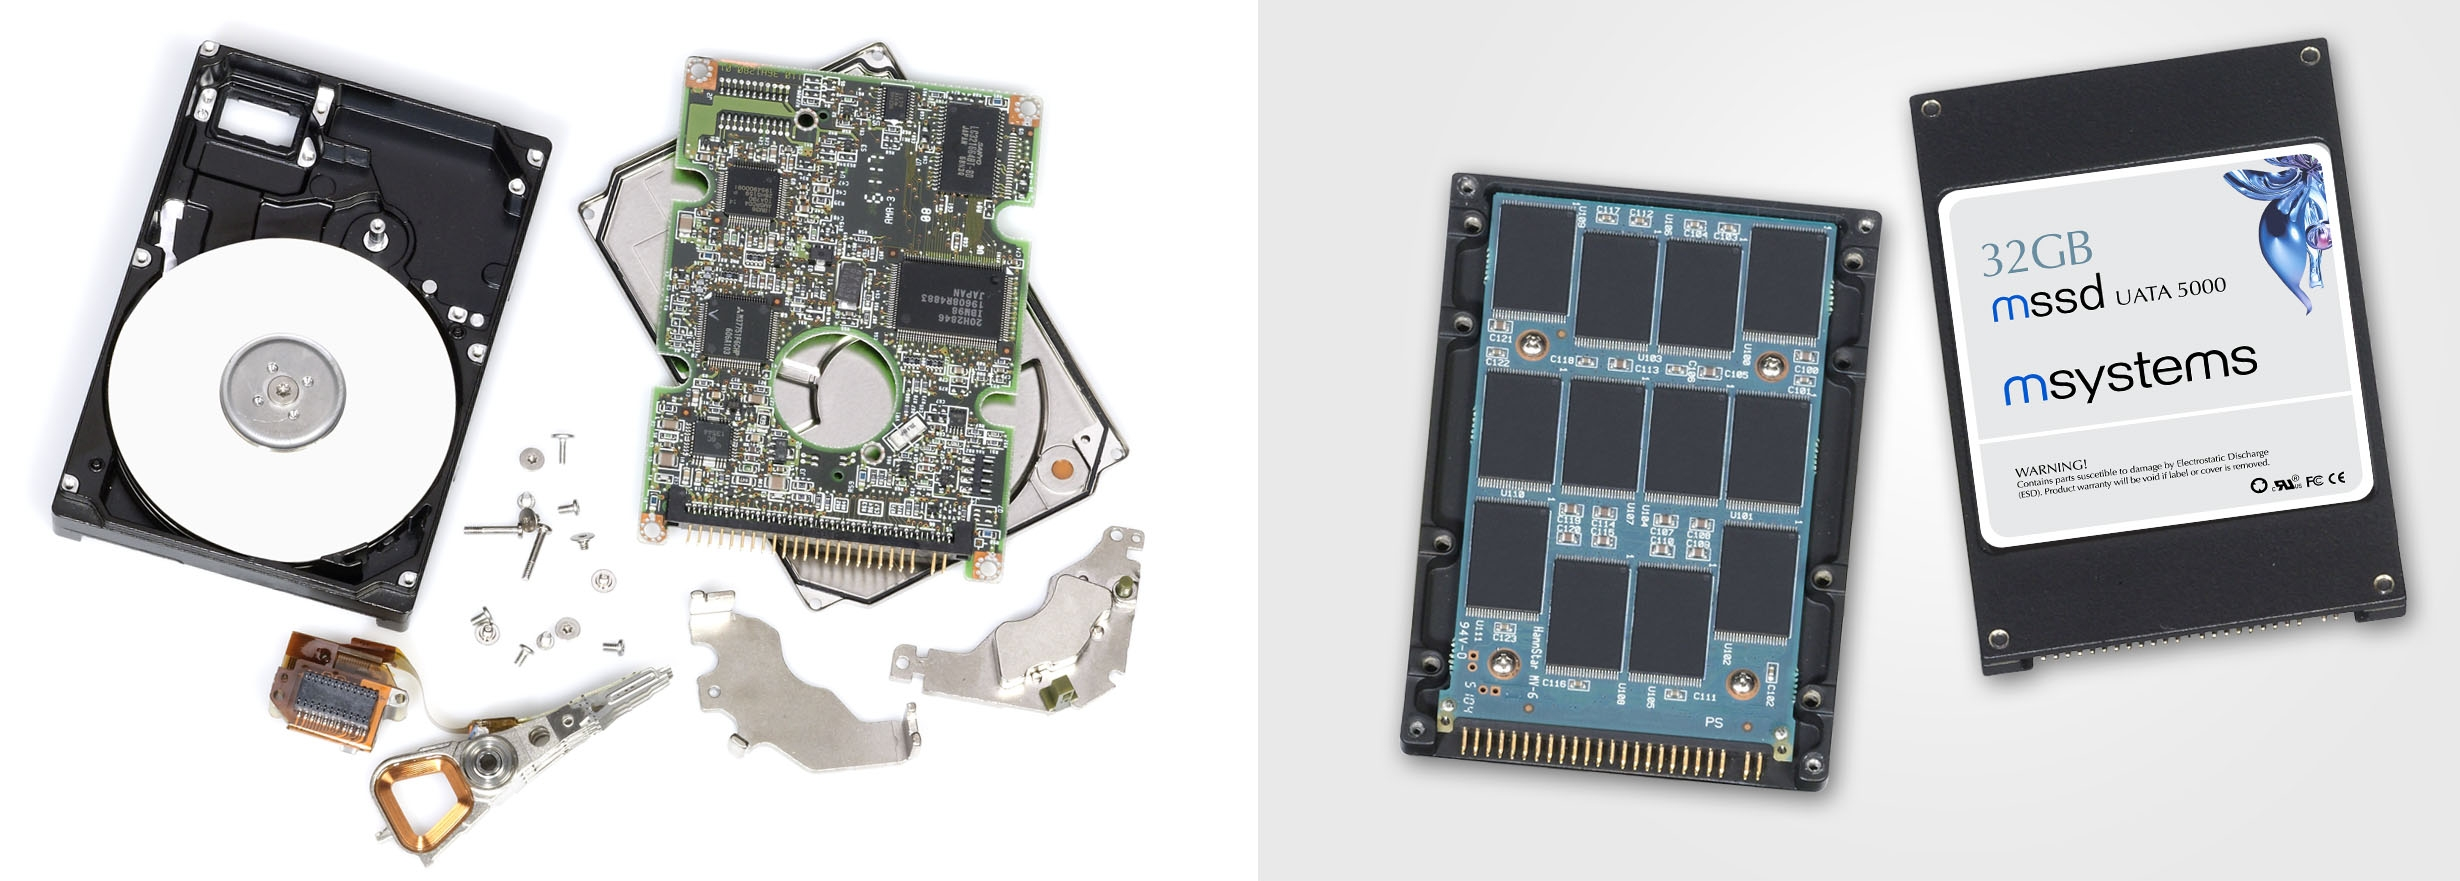
\includegraphics[width=1.0\linewidth]{images/5_memory/hdd_ssd.jpeg}
		\caption{Un comune disco rigido (a sinistra) confrontato con un'unità a stato solido (a destra)}
		\label{fig:memory_hdd_sdd}
	\end{figure}
\end{frame}


\subsubsection[Le memorie flash]{Le memorie flash}
\begin{frame}
	\frametitle{Le memorie flash}
	  
	\begin{block}{}
		Le memorie flash sono dispositivi di archiviazione a stato solido utilizzati per conservare dati in modo \textbf{non volatile}, mantenendo le informazioni anche senza alimentazione elettrica. 
		Sono cruciali per l'archiviazione di dati in una vasta gamma di dispositivi, fornendo un equilibrio tra velocità, capacità e affidabilità.
		Le memorie flash offrono un \textbf{accesso veloce} ai dati e sono \textbf{resistenti agli urti}, rendendole ideali per \textit{dispositivi mobili, penne USB, schede di memoria, SSD e altro}.\\ \vspace{0.5em}

		Esistono due tipi principali di memorie flash:
		\begin{itemize}
			\item La \textbf{NAND Flash} è più comune ed economica, adatta per lo storage di massa in dispositivi come SSD e schede di memoria.
			\item La \textbf{NOR Flash} è più veloce ma costosa, utilizzata in applicazioni che richiedono un accesso rapido ai dati come firmware di dispositivi embedded e BIOS di computer.
		\end{itemize}
		
	\end{block}
	
\end{frame}

% https://www.embedded.com/flash-101-nand-flash-vs-nor-flash/
\begin{frame}
	\frametitle{Le memorie flash}
	
	\begin{figure}[!htbp]
		\centering
		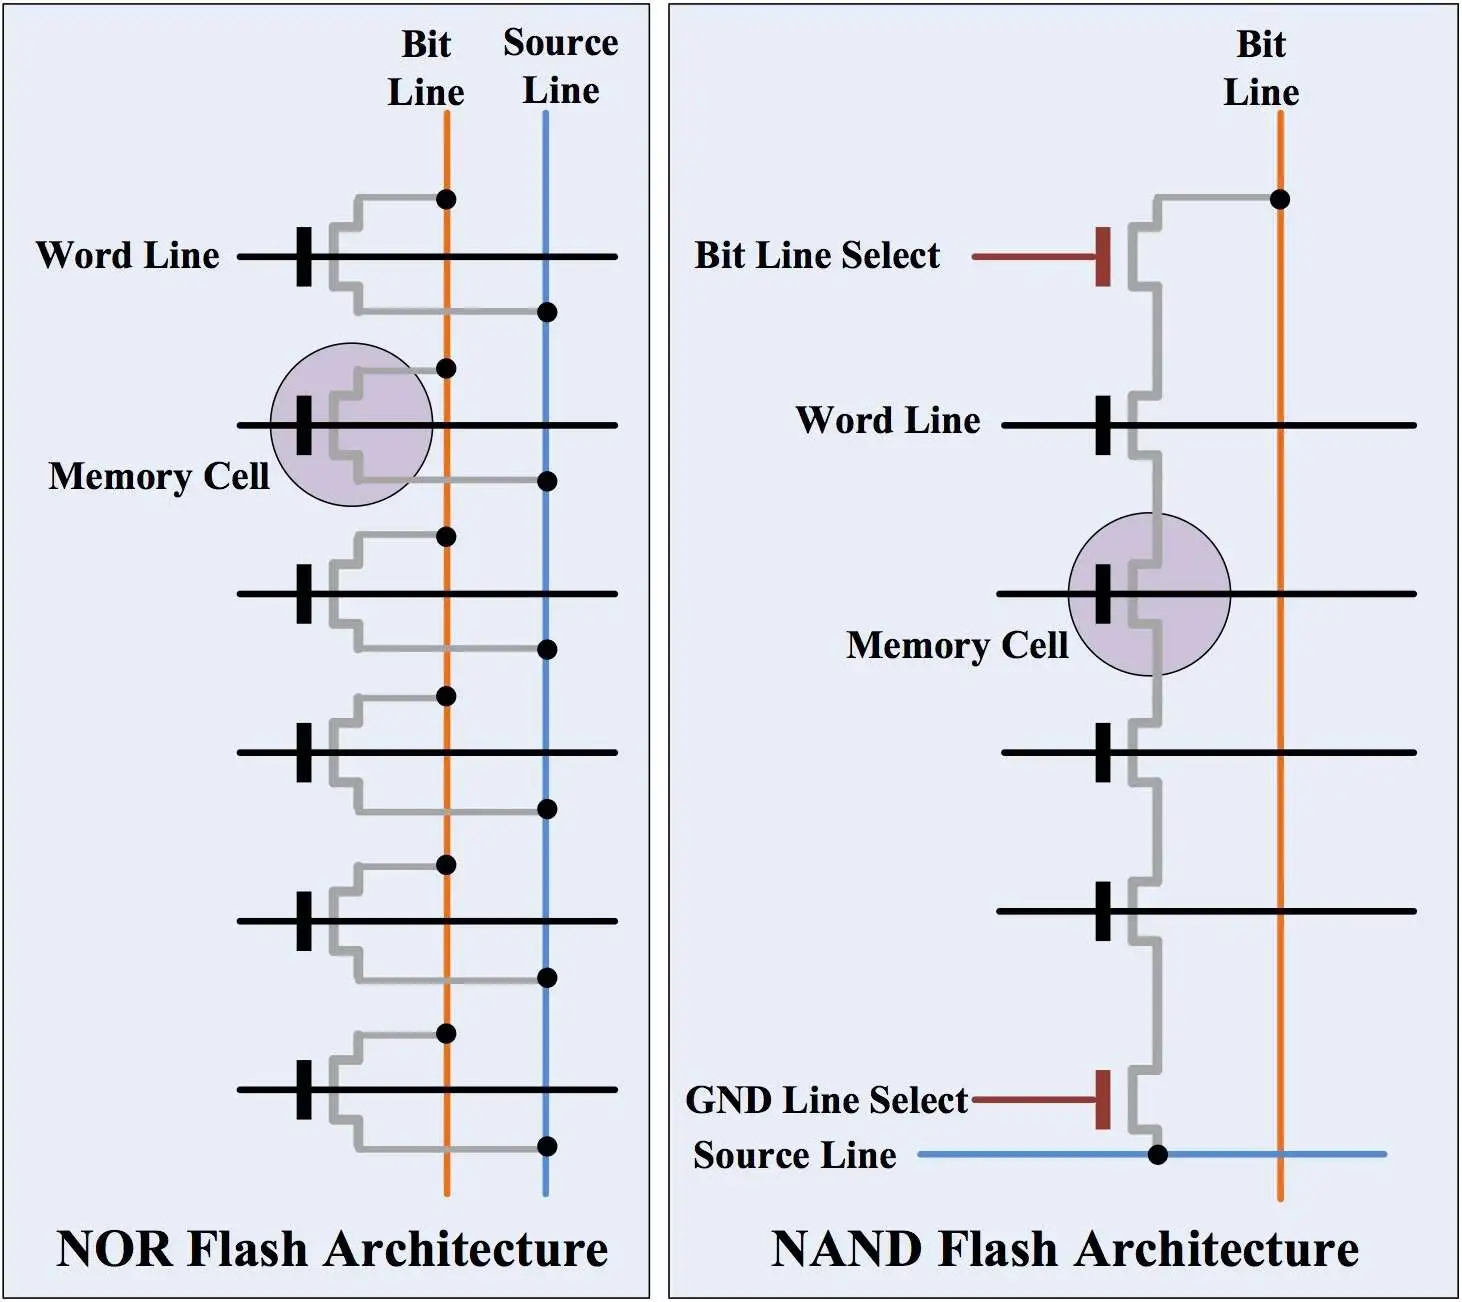
\includegraphics[width=0.57\linewidth]{images/5_memory/flash_nor_nand.png}
		\caption{NOR Flash (left) has an architecture resembling a NOR gate. Similarly, NAND Flash (right) resembles a NAND gate. (Source: Cypress)}
%			\label{fig:memory_so_dimm}
	\end{figure}
\end{frame}


\begin{frame}
	\frametitle{Le memorie flash: esempi}
	
	\begin{figure}[!htbp]
		\centering
		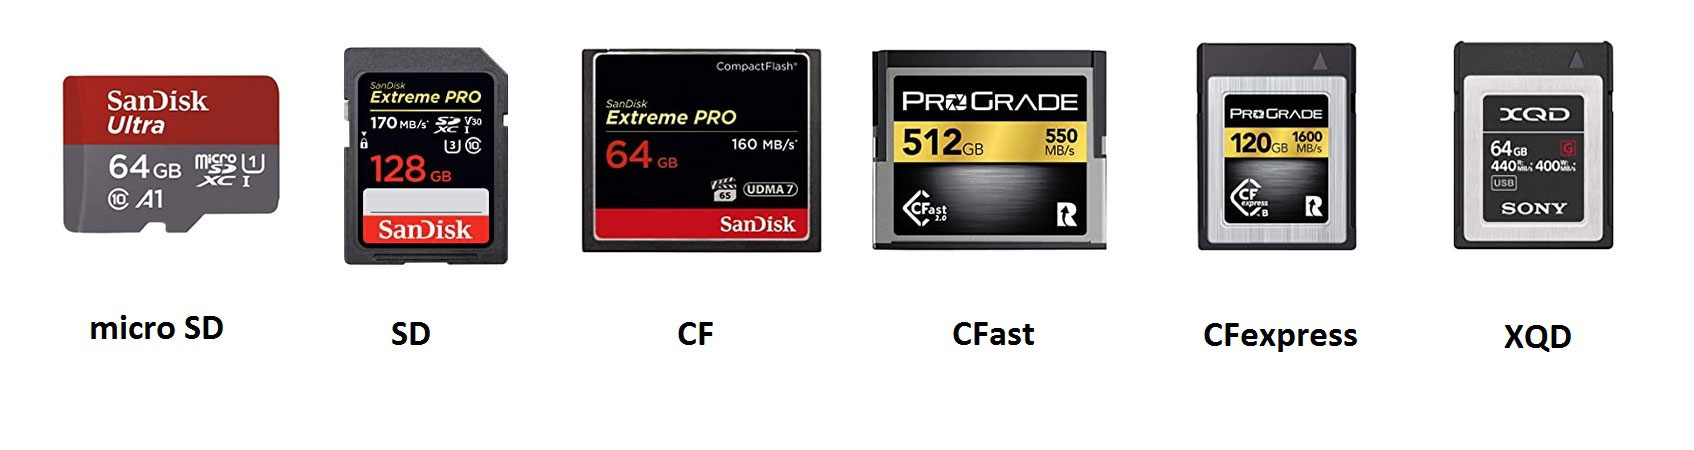
\includegraphics[width=1.0\linewidth]{images/5_memory/flash_1.jpg}
		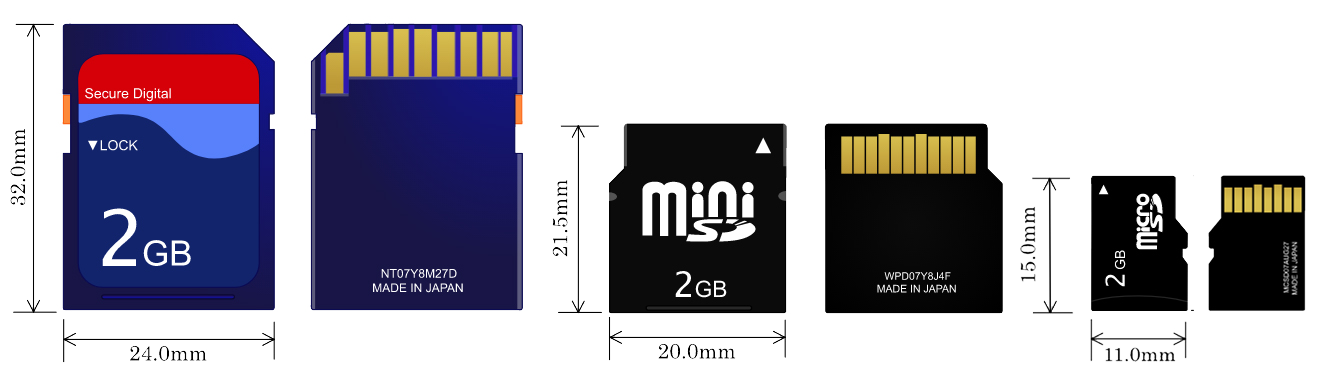
\includegraphics[width=1.0\linewidth]{images/5_memory/flash_2.png}
%		\caption{}
%		\label{fig:memory_so_dimm}
	\end{figure}
\end{frame}

% https://www.sdcard.org/developers/sd-standard-overview/speed-class/
\begin{frame}
	\frametitle{Le memorie flash: SD}
	
	\begin{figure}[!htbp]
		\centering
		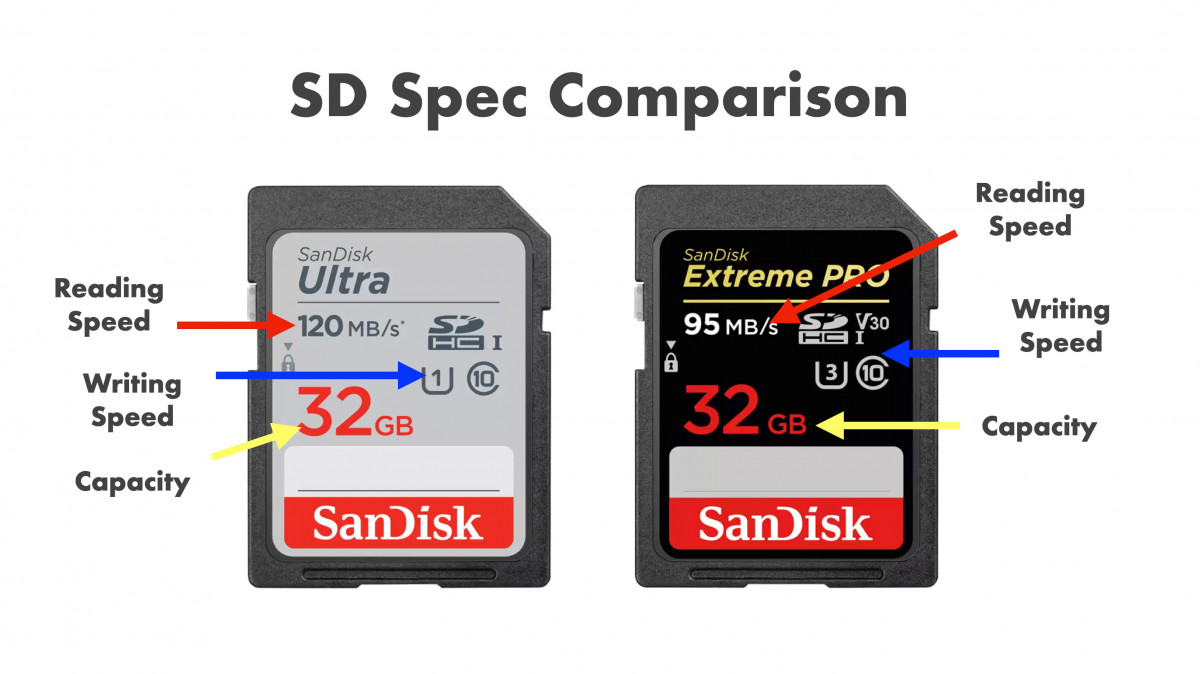
\includegraphics[width=1.0\linewidth]{images/5_memory/flash_3.jpg}
%		\caption{}
%		\label{fig:memory_so_dimm}
	\end{figure}
\end{frame}

\begin{frame}
	\frametitle{Le memorie flash: SD}
	
	\begin{figure}[!htbp]
		\centering
		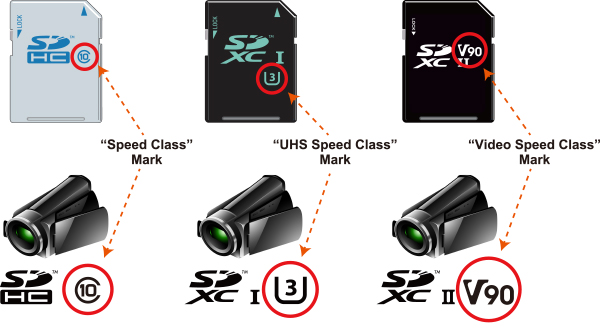
\includegraphics[width=1.0\linewidth]{images/5_memory/flash_4.jpg}
%		\caption{}
%		\label{fig:memory_so_dimm}
	\end{figure}
\end{frame}

\begin{frame}
	\frametitle{Le memorie flash: speed class}
	
	\begin{figure}[!htbp]
		\centering
		\includegraphics[width=0.55\linewidth]{images/5_memory/flash_5.png}
%		\caption{}
%		\label{fig:memory_so_dimm}
	\end{figure}
\end{frame}

\begin{frame}
	\frametitle{Le memorie flash: speed class}
	
	\begin{figure}[!htbp]
		\centering
		\includegraphics[width=1.0\linewidth]{images/5_memory/flash_6.png}
%		\caption{}
%		\label{fig:memory_so_dimm}
	\end{figure}
\end{frame}


\subsubsection[HHD]{HHD}
\begin{frame}
	\frametitle{HHD}
	  
	\begin{block}{HHD}
		Gli HDD rappresentano una delle tecnologie di archiviazione più tradizionali e sono stati a lungo il principale mezzo di archiviazione permanente nei computer. Gli HDD si basano su dischi magnetici rotanti, noti come piatti, che vengono letti e scritti da teste di lettura/scrittura mobili.\\~\\ L'informazione è memorizzata sotto forma di impulsi magnetici su questi piatti. Una maggiore capacità di archiviazione può essere ottenuta aumentando il numero di piatti all'interno dell'unità e aumentando la densità di dati su ciascun piatto.\\~\\
		Gli HDD sono generalmente apprezzati per la loro ampiezza di archiviazione e il prezzo più basso rispetto ad altre tecnologie.
	\end{block}
\end{frame}


\begin{frame}
	\frametitle{HHD}
	  
	\begin{block}{}
		 Gli HHD hanno velocità di accesso relativamente più lente rispetto agli SSD e sono sensibili a urti e movimenti bruschi, poiché le parti meccaniche all'interno possono subire danni	 
	\end{block}
	\begin{figure}[!htbp]
		\centering 
		\includegraphics[width=0.65\linewidth]{images/5_memory/hdd_info_0.pdf}
		%\caption{}
		\label{fig:memory_hdd_info_0}
	\end{figure}
\end{frame}


\begin{frame}
	\frametitle{HHD}
	  
	\begin{figure}[!htbp]
		\centering 
		\includegraphics[width=0.62\linewidth]{images/5_memory/hdd_info_1.jpg}
		%\caption{}
		\label{fig:memory_hdd_info_1}
	\end{figure}
\end{frame}




\begin{frame}
	\frametitle{HHD}
	 
%	La memoria RAM per PC viene realizzata in moduli:

	\begin{columns}			
		\column{0.5\linewidth}
		\begin{figure}[!htbp]
			\centering 
			\includegraphics[width=1.0\linewidth]{images/5_memory/hdd_info_2.png}
%			\caption{}
%			\label{fig:memory_dimm}
		\end{figure}

		\column{0.5\linewidth}
		\begin{figure}[!htbp]
			\centering 
			\includegraphics[width=1.0\linewidth]{images/5_memory/hdd_info_3.png}
%			\caption{}
%			\label{fig:memory_so_dimm}
		\end{figure}
	\end{columns}
	
\end{frame}


\begin{frame}
	\frametitle{HHD}
	 
%	La memoria RAM per PC viene realizzata in moduli:

	\begin{columns}			
		\column{0.5\linewidth}
		\begin{itemize}
			
			\item \textbf{Settore}: segmento minimo di dati su disco, solitamente 512 byte, accessibile individualmente per lettura/scrittura. 
			\item \textbf{Cluster}: gruppo di settori contigui appartenenti ad una stessa traccia.
			\item \textbf{Traccia}: cerchio concentrico su un disco che contiene dati. La \textit{traccia} è costituita da tutti i settori concentrici di un disco.
			\item \textbf{Cilindro}: insieme di tracce verticali allineate su tutti i piatti.
		\end{itemize}

		\column{0.5\linewidth}
		\begin{figure}[!htbp]
			\centering
			\includegraphics[width=1.0\linewidth]{images/5_memory/hdd_info_3.png}
%			\caption{}
%			\label{fig:memory_so_dimm}
		\end{figure}
	\end{columns}
	
\end{frame}





\subsubsection[SDD]{SDD}
\begin{frame}
	\frametitle{SDD}
	  
	\begin{block}{SDD}
		Gli SSD sono una tecnologia più recente e si sono rapidamente affermati come alternativa di archiviazione altamente performante agli HDD. A differenza degli HDD, gli SSD non hanno parti mobili; invece, utilizzano chip di memoria flash per memorizzare dati in modo permanente. Questa tecnologia permette tempi di accesso notevolmente più rapidi rispetto agli HDD, migliorando notevolmente la reattività del sistema operativo e dei programmi.\\~\\
		Gli SSD sono anche noti per la loro maggiore resistenza agli urti e ai movimenti bruschi, poiché non hanno parti meccaniche soggette a usura. Tuttavia, a causa delle loro caratteristiche di memoria flash, gli SSD tendono a avere una vita utile limitata rispetto agli HDD.
	\end{block}
\end{frame}


\begin{frame}
	\frametitle{SSD}
	 
	\begin{columns}
		\column{0.5\linewidth}
		\begin{figure}[!htbp]
			\centering 
			\includegraphics[width=1.0\linewidth]{images/5_memory/ssd_info_1.png}
%			\caption{}
%			\label{}
		\end{figure}
			
		\column{0.5\linewidth}
		\begin{figure}[!htbp]
			\centering 
			\includegraphics[width=1.0\linewidth]{images/5_memory/ssd_info_2.png}
%			\caption{}
%			\label{}
		\end{figure}
	\end{columns}
	
\end{frame}

\begin{frame}
	\frametitle{SSD}
	  
	\begin{figure}[!htbp]
		\centering 
		\includegraphics[width=0.55\linewidth]{images/5_memory/ssd_info_3.jpg}
		%\caption{}
		\label{fig:memory_ssd_info_0}
	\end{figure}
\end{frame}


\begin{frame}
	\frametitle{SSD: per notebooks}
	  
	\begin{figure}[!htbp]
		\centering 
		\includegraphics[width=1.0\linewidth]{images/5_memory/ssd_info_4.png}
		%\caption{}
%		\label{}
	\end{figure}
\end{frame}



\subsubsection[HDD vs SSD]{HDD vs SSD}
\begin{frame}
	\frametitle{HDD vs SSD}
	  
	\begin{block}{HDD vs SSD}
	
		La differenza tra dischi rigidi e unità a stato solido è nella tecnologia utilizzata per archiviare e recuperare i dati. La tabella seguente illustra alcune delle differenze. Gli HDD sono più economici e puoi ottenere più spazio di archiviazione a parità di costo. Gli SSD, tuttavia, sono incredibilmente più veloci, più leggeri, più durevoli e consumano meno energia.
	\end{block}
	\begin{table}[]
			\begin{tabular}{|c |
			>{\columncolor[HTML]{C0C0C0}}c |
			>{\columncolor[HTML]{C0C0C0}}c |
			}
			\hline
			\cellcolor[HTML]{FFFFFF}\textbf{$$} & \cellcolor[HTML]{EFEFEF}\textbf{$\pmb{HHD}$} & \cellcolor[HTML]{EFEFEF}$\pmb{SSD}$ \\ \hline
			\textbf{Cost} & Cheaper & More expensive \\ \hline
			\textbf{Speed} & Slower & Faster \\ \hline
			\textbf{Durability} & Less Durable & More Durable \\ \hline
			\textbf{Energy Efficency} & Use more energy & Use less energy \\ \hline
			\textbf{Noisiness} & Noisy & Absent \\ \hline
			\textbf{Warm Produced} & More & Less \\ \hline
			\end{tabular}
		\end{table}
\end{frame}


\begin{frame}
	\frametitle{HDD vs SSD}
	  
	\begin{figure}[!htbp]
		\centering 
		\includegraphics[width=1.0\linewidth]{images/5_memory/hhd_vs_ssd.jpg}
		%\caption{}
%		\label{}
	\end{figure}
\end{frame}

